% Header
\renewcommand\evenpagerightmark{{\scshape\small Chapter 6}}
\renewcommand\oddpageleftmark{{\scshape\small Improved RPC investigation and preliminary electronics studies}}

\renewcommand{\bibname}{References}

\hyphenation{}

\chapter[Improved RPC investigation and preliminary electronics studies]%
{Improved RPC investigation and preliminary electronics studies}
\label{chapt6}

	The extension in the endcap of the RPC sub-system towards higher pseudo-rapidity will bring the new detectors to be exposed to much more intense background radiations due to the proximity of the detectors with the beam line (Figure~\ref{fig:Dose}). The challenge will be to produce high counting rate detectors with limited ageing rate to ensure a stable operation of the detector over a period longer than ten years. In Chapter~\ref{chapt3} was discussed the influence of the detector design (the number and the thickness of the gas volumes, double-gap design, etc...) on the charge deposition and rate capability. Nevertheless, this question can also be addressed from the electronics point of view as a better signal-to-noise ratio would also mean the possibility to greatly lower the charge threshold on the signals to be detected, allowing to use the detector at lower gain, hence lowering the charge deposition per avalanche in the gas volume. Cardarelli showed that the production of low-noise fast FEEs could help decreasing the charge deposition per avalanche at working voltage by an order of magnitude, virtually increasing the life expectancy of such a detector in the same way~\cite{CARDARELLI2012}.
	
	In this Chapter, the electronics that were chosen to equip the improved RPCs (iRPCs) will be presented. These electronics are the based on the PETIROC ASIC. A similar technology has been previously used with RPCs in the context of the R\&D of a \acf{SDHCAL} for the \acf{ILD}. As back-up to the PETIROC, a FEB developed by the INFN Tor Vergata in Rome as also been studied for the CMS iRPCs.\\
	These two solutions for the iRPCs are the results of a longer selection process in which I took a great part. Thus, after an introduction of both technologies, the tests performed on CMS RPCs operated with preliminary versions of INFN Tor Vergata preamplifiers as well as with the HARDROC 2 read-out panel of the SDHCAL will be discussed in details. Finally, the current status of the R\&D certification will be presented. Nonetheless, it is important to keep in mind that I did not personally participate in the development of the PETIROC FEB nor of the INFN Tor Vergata FEB as designed for the iRPCs. My role was limited to the selection and to the test of potential candidates. After this preliminary study was conducted, the development of the actual FEEs for the CMS iRPCs was conducted by other researchers. Therefore, I will only report the status of the ongoing research.

\section{FEE candidates for the production of iRPCs}
\label{chapt6:sec:candidates}

	The extension of the third and fourth endcap disks with \acl{iRPC}s has been presented in Chapter~\ref{chapt:4} together with the expected background levels (Figure~\ref{fig:iRPC-Rate}). The iRPCs will complete the muon endcap as described in Figure~\ref{fig:iRPC-Wheel}. The key features of these iRPCs are:

	\begin{itemize}
		\item double-gap design,
		\item \SI{1.4}{mm} thick HPL electrodes,
		\item 0.9 to \Sci{3}{10}\,\si{\ohm\cdot cm} HPL resistivity,
		\item \SI{1.4}{mm} thick gas gap,
		\item trapezoidal chambers spanning \SI{20}{\degree} in $\varphi$ around the beam axis,
		\item read-out panel consisting of 96 trapezoidal strips
		\item strip pitch ranges from \SI{6.0}{mm} (\SI{5.9}{mm}) on the high pseudo-rapidity end to \SI{12.3}{mm} (\SI{10.9}{mm}) on the low one on position RE3/1 (RE4/1)
		\item spatial resolution in the direction perpendicular to the strips $\sim$\SI{3}{mm}
	\end{itemize}
	
	\begin{figure}[H]
		\centering
		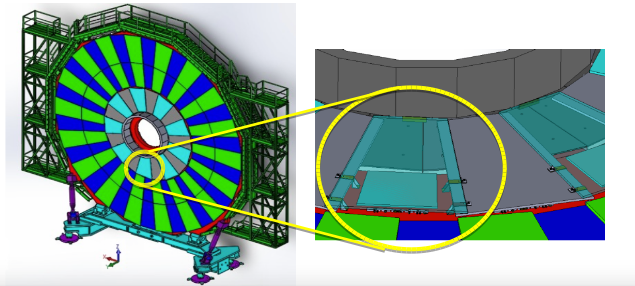
\includegraphics[width = \linewidth]{fig/chapt6/iRPC-Wheel.png}\\
		\caption{\label{fig:iRPC-Wheel} Location of the RE3/1 or RE4/1 iRPCs on a muon endcap disk.}
	\end{figure}

	An important piece of these iRPCs will be the \acl{FEE} that will equip the chambers. A fast, low-jitter and low-charge sensitive electronics will help reducing further the charge deposition in the detector by making it possible to operate at lower gain. The FEEs that are foreseen to equip the new RPCs need to be able to detect charges as small as \SI{10}{fC}. Not only the new electronics need to be fast and reliable, they also should be able to sustain the high radiation the detectors will be subjected to in the region closest to the beam.
	
	\subsection{PETIROC: the RPC upgrade baseline}
	\label{chapt6:ssec:RPCROC}
	
	Designed by Weeroc, a spin-off company from the OMEGA Collaboration, the PETIROC 2A consits in a fast and low jitter 32-channel ASIC originally developed to read-out \acf{SiPM} in ToF applications and that allows for precise time measurements~\cite{PETIROCIEEE,PETIROCTWEPP}. The ASIC uses an AMS \SI{350}{ns} \acf{SiGe} technology. The block diagram of the ASIC is shown on Figure~\ref{fig:PETIROCASIC}. A 10-bit DAC allows to adjust the trigger level in a dynamical range spanning from 0.5 to a few tens of photoelectrons and a 6-bit DAC to adjust the response of each individual channel to similar a level.
	
	\begin{figure}[H]
		\centering
		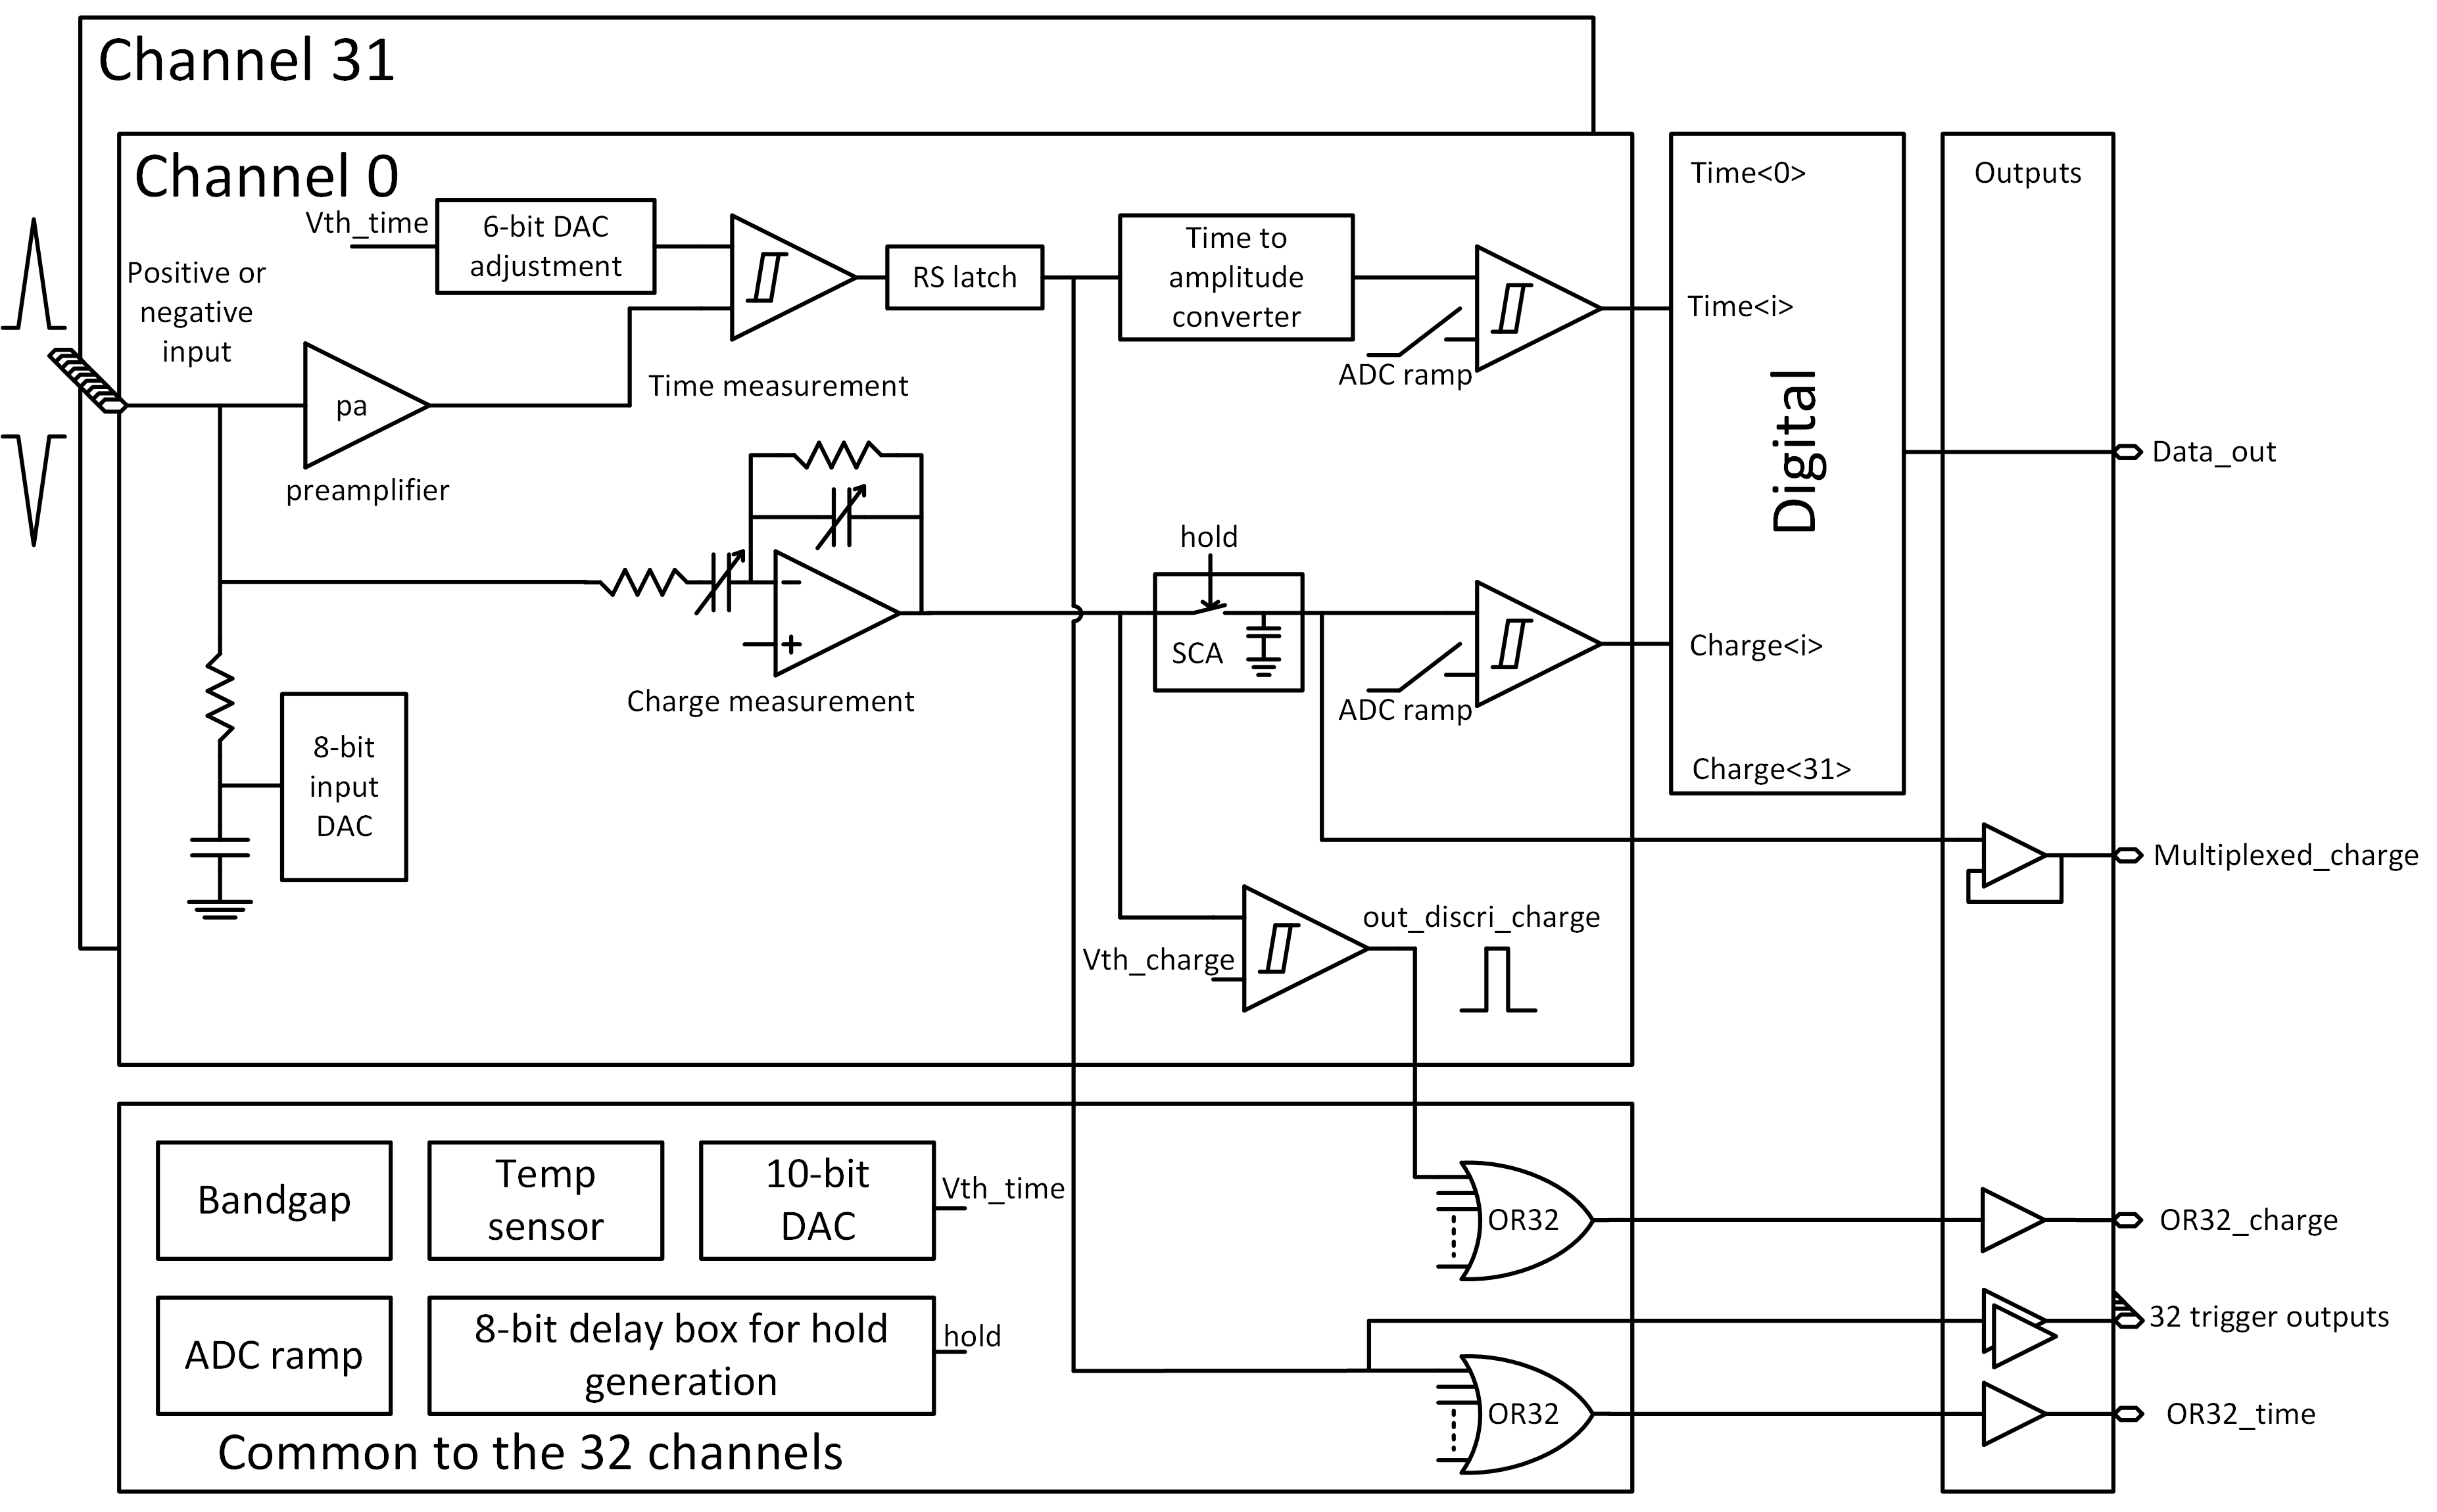
\includegraphics[width = \linewidth]{fig/chapt6/petiroc2.png}\\
		\caption{\label{fig:PETIROCASIC} PETIROC 2A block diagram.}
	\end{figure}
	
	Nevertheless, to adapt this ASIC to CMS, modifications were brought to the PETIROC~\cite{PHASEIITP} and not all its functions will be used~\cite{COMBARET2018}. Due to the radiation levels that are foreseen at the level of the iRPCs, the SiGe technology will be replaced by the Taiwan Semiconductor Manufacturing Company (TSMC) \SI{130}{nm} CMOS, to increase its radiation hardness while keeping fast pre-amplification and discrimination. On the \acl{FEB}, the ASIC is associated with an FPGA which purpose is to measure the arrival time of the signals. The FPGA is equipped with a TDC with a time resolution of 50-100 \si{ps} developed by Tsinghua University. The full system will provide a measurement of the signal position along the strip with a precision of a few \si{cm} by reading the signal on both strip ends. Finally, the measurement of the charge will be performed by a \acf{ToT} technic, taking profit of the capacity the ASIC in measuring both the leading and trailing edges of the input signals.
	
	\newpage

	\begin{figure}[H]
		\begin{subfigure}{0.5\linewidth}
		    \centering
			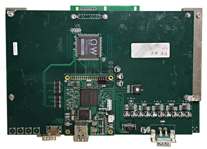
\includegraphics[width = 0.8\linewidth]{fig/chapt6/iRPC-RPCROCv0.png}
			\caption{\label{fig:RPCROC_FEB:A}}
		\end{subfigure}
		\begin{subfigure}{0.5\linewidth}
		    \centering
			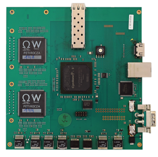
\includegraphics[width = 0.7\linewidth]{fig/chapt6/iRPC-RPCROCv1.png}
			\caption{\label{fig:RPCROC_FEB:B}}
		\end{subfigure}
		\caption{\label{fig:RPCROC_FEB} \subref{fig:RPCROC_FEB:A} View of the FEBv0 in which the PETIROC 2A ASIC is visible as well as the FPGA on which the TDC is hosted. \subref{fig:RPCROC_FEB:B} View of the FEBv1 with its two PETIROC 2A ASICs. The FPGA with the TDC is this time embedded in the FEB.}
	\end{figure}

	\begin{figure}[H]
		\begin{subfigure}{0.4\linewidth}
		    \centering
			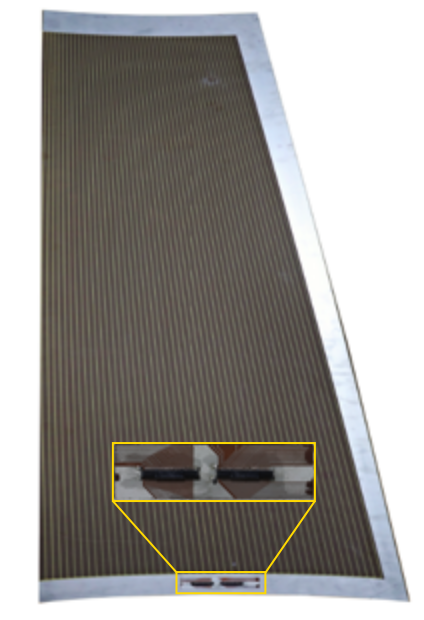
\includegraphics[width = \linewidth]{fig/chapt6/iRPC-RPCROC-PCB.png}
			\caption{\label{fig:RPCROC_FEB:A}}
		\end{subfigure}
		\begin{subfigure}{0.6\linewidth}
		    \centering
			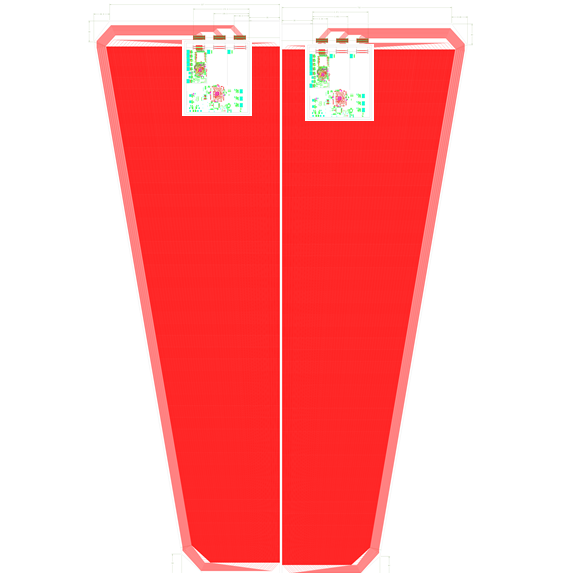
\includegraphics[width = \linewidth]{fig/chapt6/iRPC-RPCROC-Final.png}
			\caption{\label{fig:RPCROC_FEB:B}}
		\end{subfigure}
		\caption{\label{fig:RPCROC_FEB} \subref{fig:RPCROC_FEB:A} Picture of half the read-out PCB used with FEBv1. The FEB is connected directly onto the return connectors on the wide end of the panel. \subref{fig:RPCROC_FEB:B} Design of the foreseen final read-out of the iRPC showing the 2 FEBs and the read-out PCB.}
	\end{figure}
	
	Two consecutive versions of the PETIROC FEB are shown in Figure~\ref{fig:RPCROC_FEB}. FEBv0 was equipped with a single PETIROC 2A associated to a Cyclone II FPGA. FEBv1 was in turn equipped with two PETIROC 2A and then, in a later version, with two PETIROC 2B. In both cases, the ASICs were associated to a Cyclone V FPGA. The PETIROC 2B was a version of the ASIC with less cross-talk than the 2A. The dynamic range could then be expanded towards lower values to allow for the detection of charges as low as \SI{50}{fC}. The next version, the FEBv2 is expected to be equipped with three PETIROC 2C, the new generation of the ASIC, associated to three Cyclone V FPGAs hosting the 32-channel TDCs and a master Cyclone V FPGA for the communications of the TDCs with the Link-Board system. The version 2C will focus on reducing the dead-time of \SI{10}{ns} of the ASIC. Also, the Cyclone V FPGAs of the FEBv2 will use a different technology than the one used for FEBv1. The choice has been made to use a radiation tolerant PolarFire FPGA which uses data scrubbing to detect and correct errors before they accumulate. This technology is for example used for space applications. The FEB will be tested at the \acf{LLN} neutron beam. The goal is to irradiate the electronics up to a fluence of \Ord{14}\,\si{pC/cm^2}, five times more than what is expected at CMS, to certify its radiation hardness.\\
	Each FEBv2 will be able to read 96 channels out thanks to three 32-channel PETIROC 2C ASICs. Two FEBv2 would be mounted on the iRPC to read the 96 strips out from both ends. The read-out panel that was used for the first version of the FEB is shown in Figure~\ref{fig:RPCROC_FEB:A} and the final design with the FEBv2 mounted on the read-out plane is shown in Figure~\ref{fig:RPCROC_FEB:B}.

	\subsection{INFN FEB: a robust back-up solution}
	\label{chapt6:ssec:INFN}
	
	Even though the baseline for the electronics that will equip the iRPCs will be the PETIROC, a back-up solution needs to be certified. The back-up has been found in \acl{FEE} featuring a fast and low-noise (1000 $e^-$ rms) Silicon (Si) preamplifier and a SiGe discriminator~\cite{PIZZIMENTO2018} associated with an optimized read-out panel~\cite{ALUNNOCAMELIA2018}. The low-noise preamplifier is a new version of a preliminary production of a SiGe preamplifier by the team of Cardarelli working with INFN Tor Vergata in Rome with the purpose of equipping the new generation of ATLAS RPCs~\cite{CARDARELLI2013}. The study of the early version of the preamplifier by is discussed in Section~\ref{chapt6:sec:Preliminary}.
	 
	\begin{figure}[H]
		\centering
		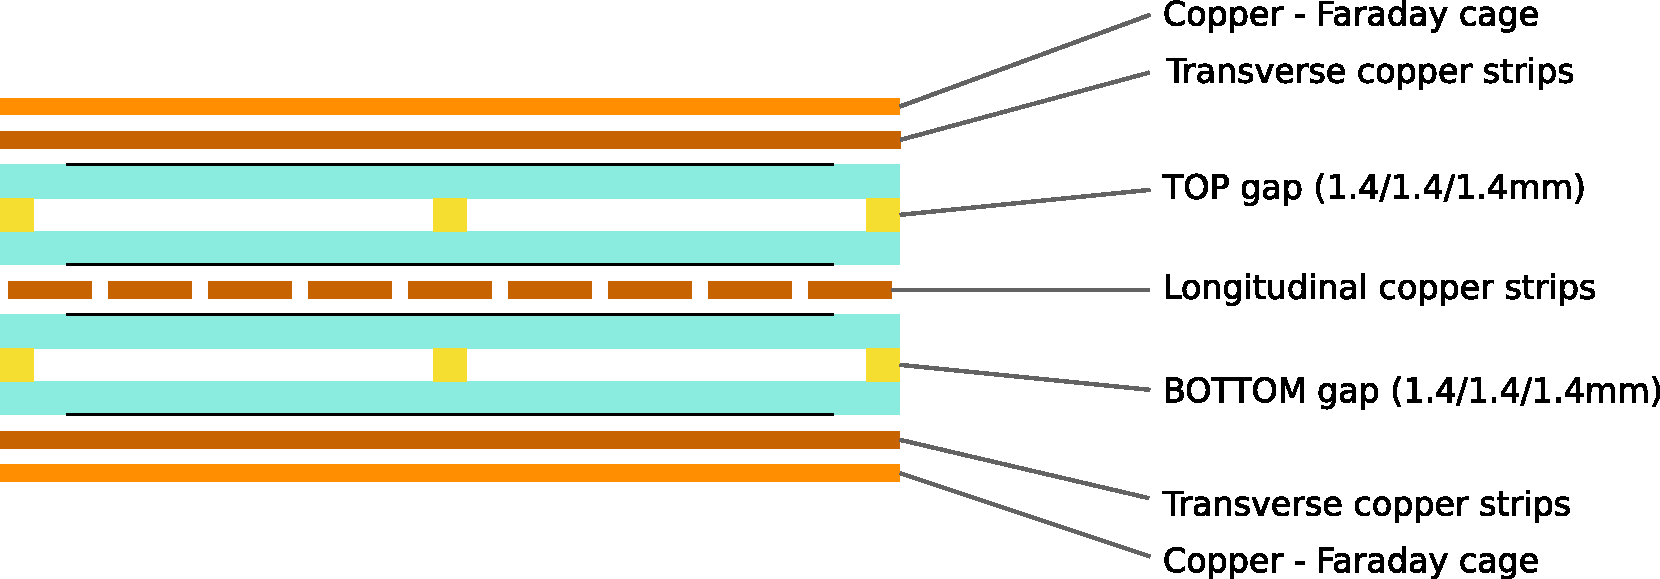
\includegraphics[width = 0.8\linewidth]{fig/chapt6/iRPC-INFN-Design.pdf}
		\caption{\label{fig:INFN-Design} Design of the iRPC in the back-up scenario. The detector includes an additional two layers of transversal strips to gain in spatial resolution.}
    \end{figure}
	
	Contrary to the PETIROC FEB, the back-up electronics only offer the possibility to read the 96 strips out from one end. The spatial resolution along the strips is then brought by two transverse strip planes. These two additional panels sandwich the double-gap ensemble as shown is Figure~\ref{fig:INFN-Design}. They feature \SI{5}{cm} wide copper strips for a spatial resolution of a few centimeters along the longitudinal strips. A top quarter of the longitudinal and transversal read-out panels is shown in Figure~\ref{fig:INFN_Readout} and pictures are available in Figure~\ref{fig:INFN_StripPic}.
	 
	\begin{figure}[H]
		\begin{subfigure}{.5\linewidth}
		    \centering
			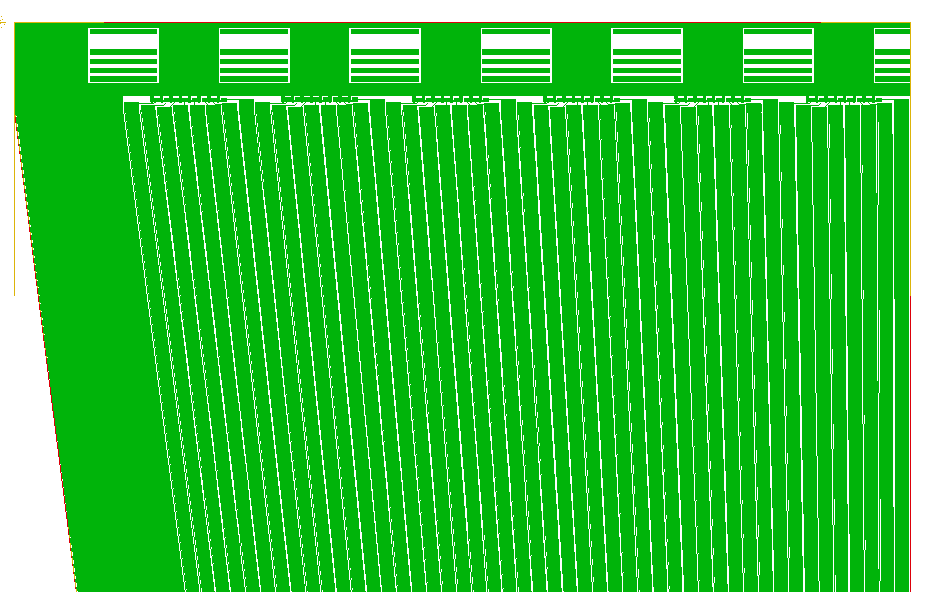
\includegraphics[width = \linewidth]{fig/chapt6/INFN-FEB-Longitudinal-Drawing.png}
			\caption{\label{fig:INFN_Readout:A}}
		\end{subfigure}
		\begin{subfigure}{.5\linewidth}
		    \centering
			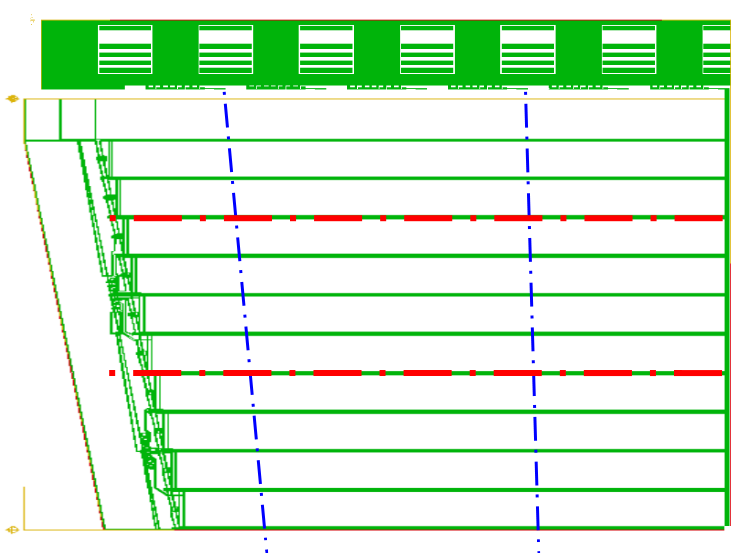
\includegraphics[width = .9\linewidth]{fig/chapt6/INFN-FEB-Transversal-Drawing.png}
			\caption{\label{fig:INFN_Readout:B}}
		\end{subfigure}
		\caption{\label{fig:INFN_Readout} Design of the longitudinal \subref{fig:INFN_Readout:A} and transversal \subref{fig:INFN_Readout:B} strip panels. The transversal design is here shown on top of the longitudinal one.}
    \end{figure}
    
    \begin{figure}[H]
		\begin{subfigure}{.5\linewidth}
		    \centering
			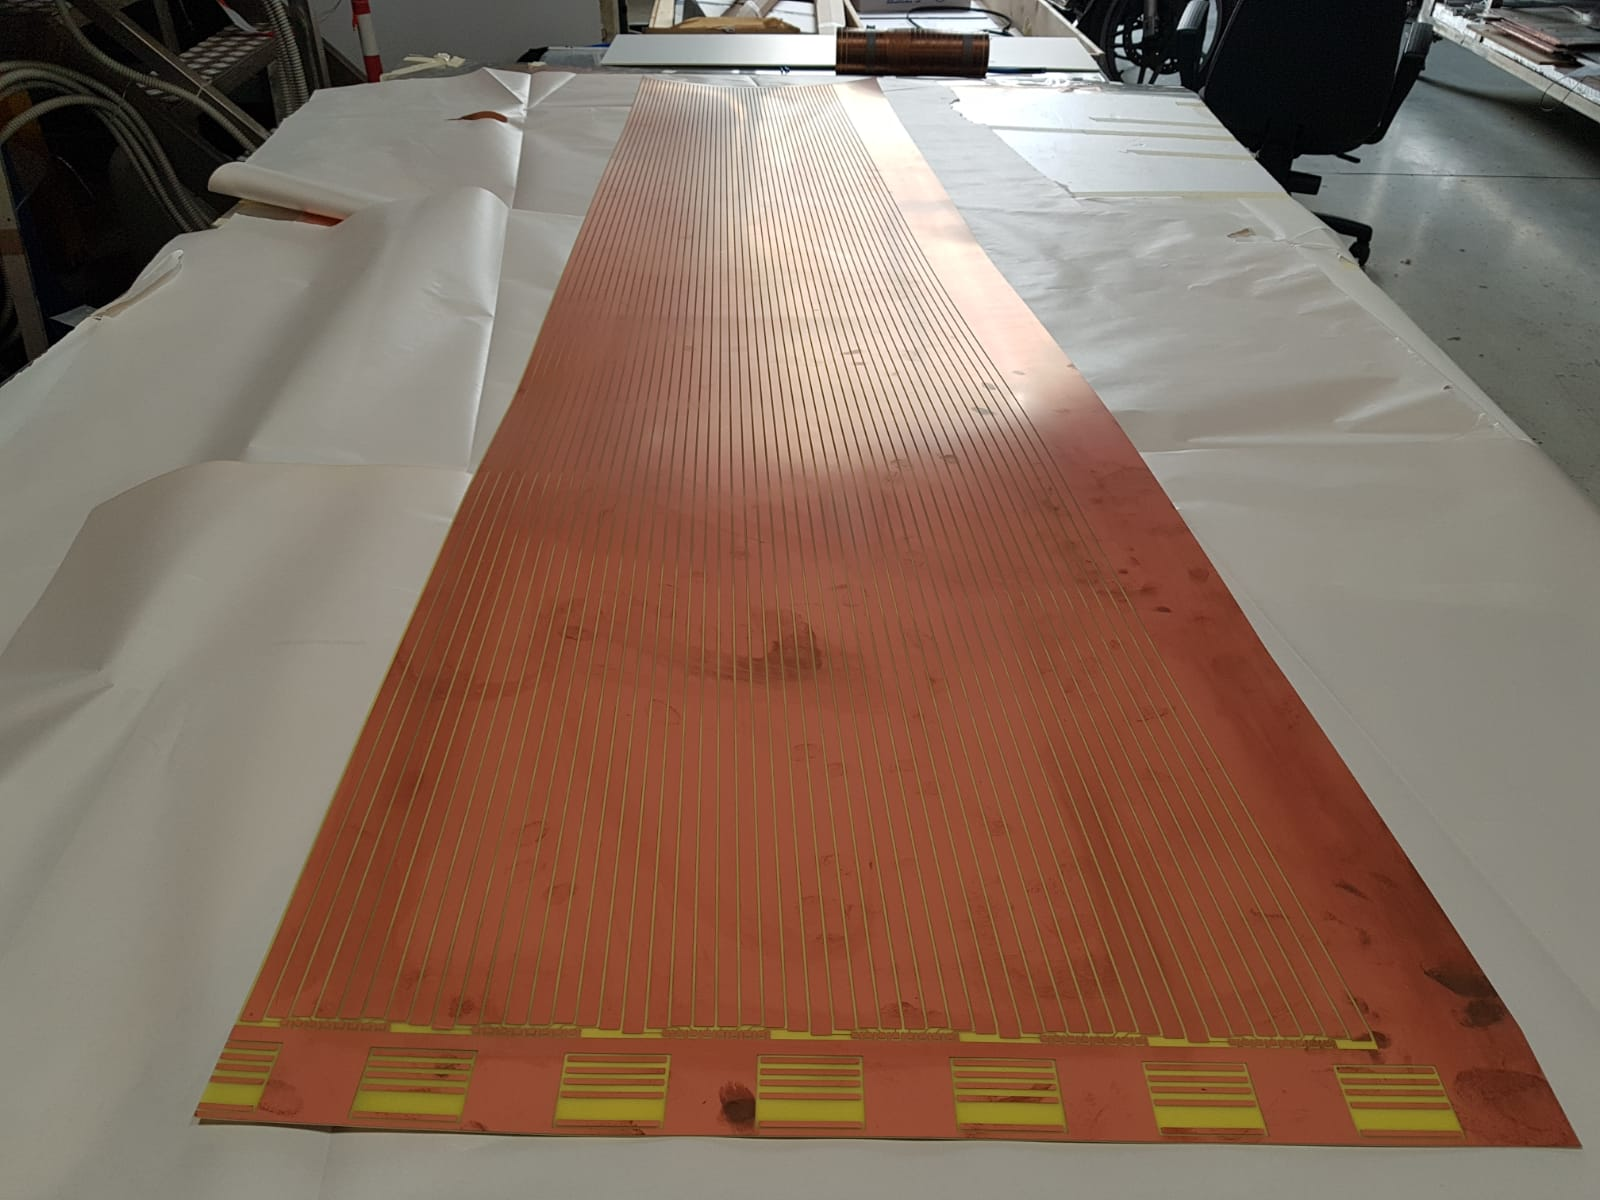
\includegraphics[width = .9\linewidth]{fig/chapt6/INFN-FEB-Longitudinal.png}
			\caption{\label{fig:INFN_StripPic:A}}
		\end{subfigure}
		\begin{subfigure}{.5\linewidth}
		    \centering
			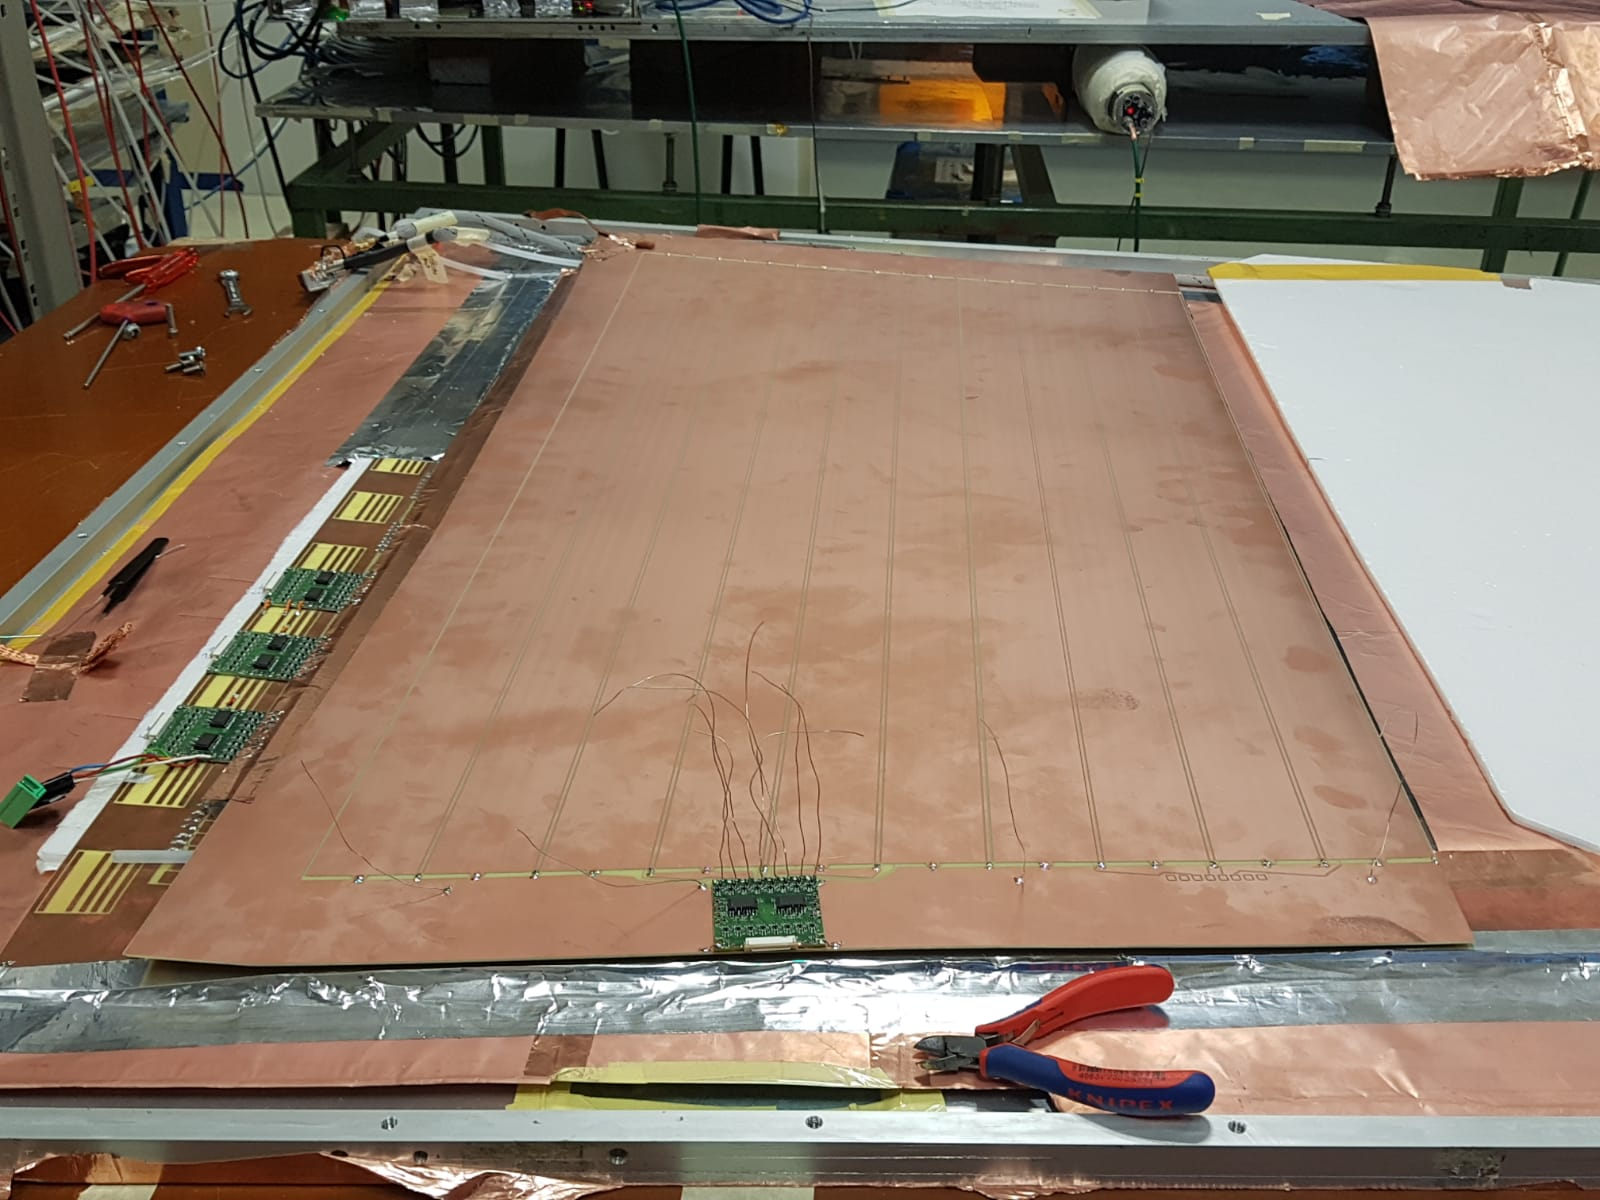
\includegraphics[width = .9\linewidth]{fig/chapt6/INFN-FEB-Transversal.png}
			\caption{\label{fig:INFN_StripPic:B}}
		\end{subfigure}
		\caption{\label{fig:INFN_StripPic} Picture of half the longitudinal \subref{fig:INFN_Readout:A} and of the top part of the transversal \subref{fig:INFN_Readout:B} strip panels.}
    \end{figure}
	
	The FEB used for the longitudinal readout is shown in Figure~\ref{fig:INFN_FEBv2:A}. Each FEB is equipped with eight preamplifiers using a \acf{BJT} technology and two discriminator ASICs of four channels using \acf{HJT} technology. The input signals are amplified at an amplification factor of 0.2 to \SI{0.4}{mV/fC} and are then discriminated with a threshold of \SI{0.5}{mV} at minimum. For each channel, the LVDS output is proportional in width to the \acl{ToT} in the discriminator of the amplified signal with a minimum width of \SI{3}{ns}. This method allows for an estimation of the avalanche charge as the width of the signals usually is consistent and proportional to the amount of charge released in the gas volume.\\
	On Figure~\ref{fig:INFN_Readout:A}, the rectangular zones with straight copper lines at the top of the longitudinal PCB are lines used to propagate the power and the slow control of the FEBs. A FEB is placed between two zones and soldered to the copper lines on both sides, as can be seen in Figure~\ref{fig:INFN_FEBv2:B}. In the same way, the FEB is soldered to a group of eight strips which lines finish into pads placed below the bottom edge of the FEB. It was decided to solder the FEBs onto the read-out PCB to reduce the pick-up noise in the electronics.
	 
	\begin{figure}[H]
		\begin{subfigure}{.6\linewidth}
		    \centering
			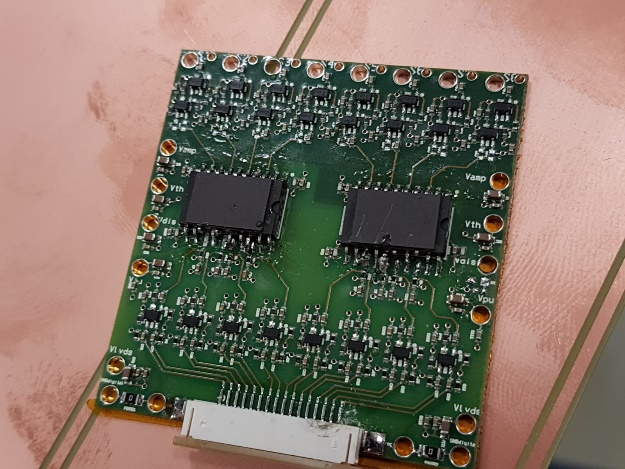
\includegraphics[height = 6cm]{fig/chapt6/INFN-FEB.png}
			\caption{\label{fig:INFN_FEBv2:A}}
		\end{subfigure}
		\begin{subfigure}{.4\linewidth}
		    \centering
			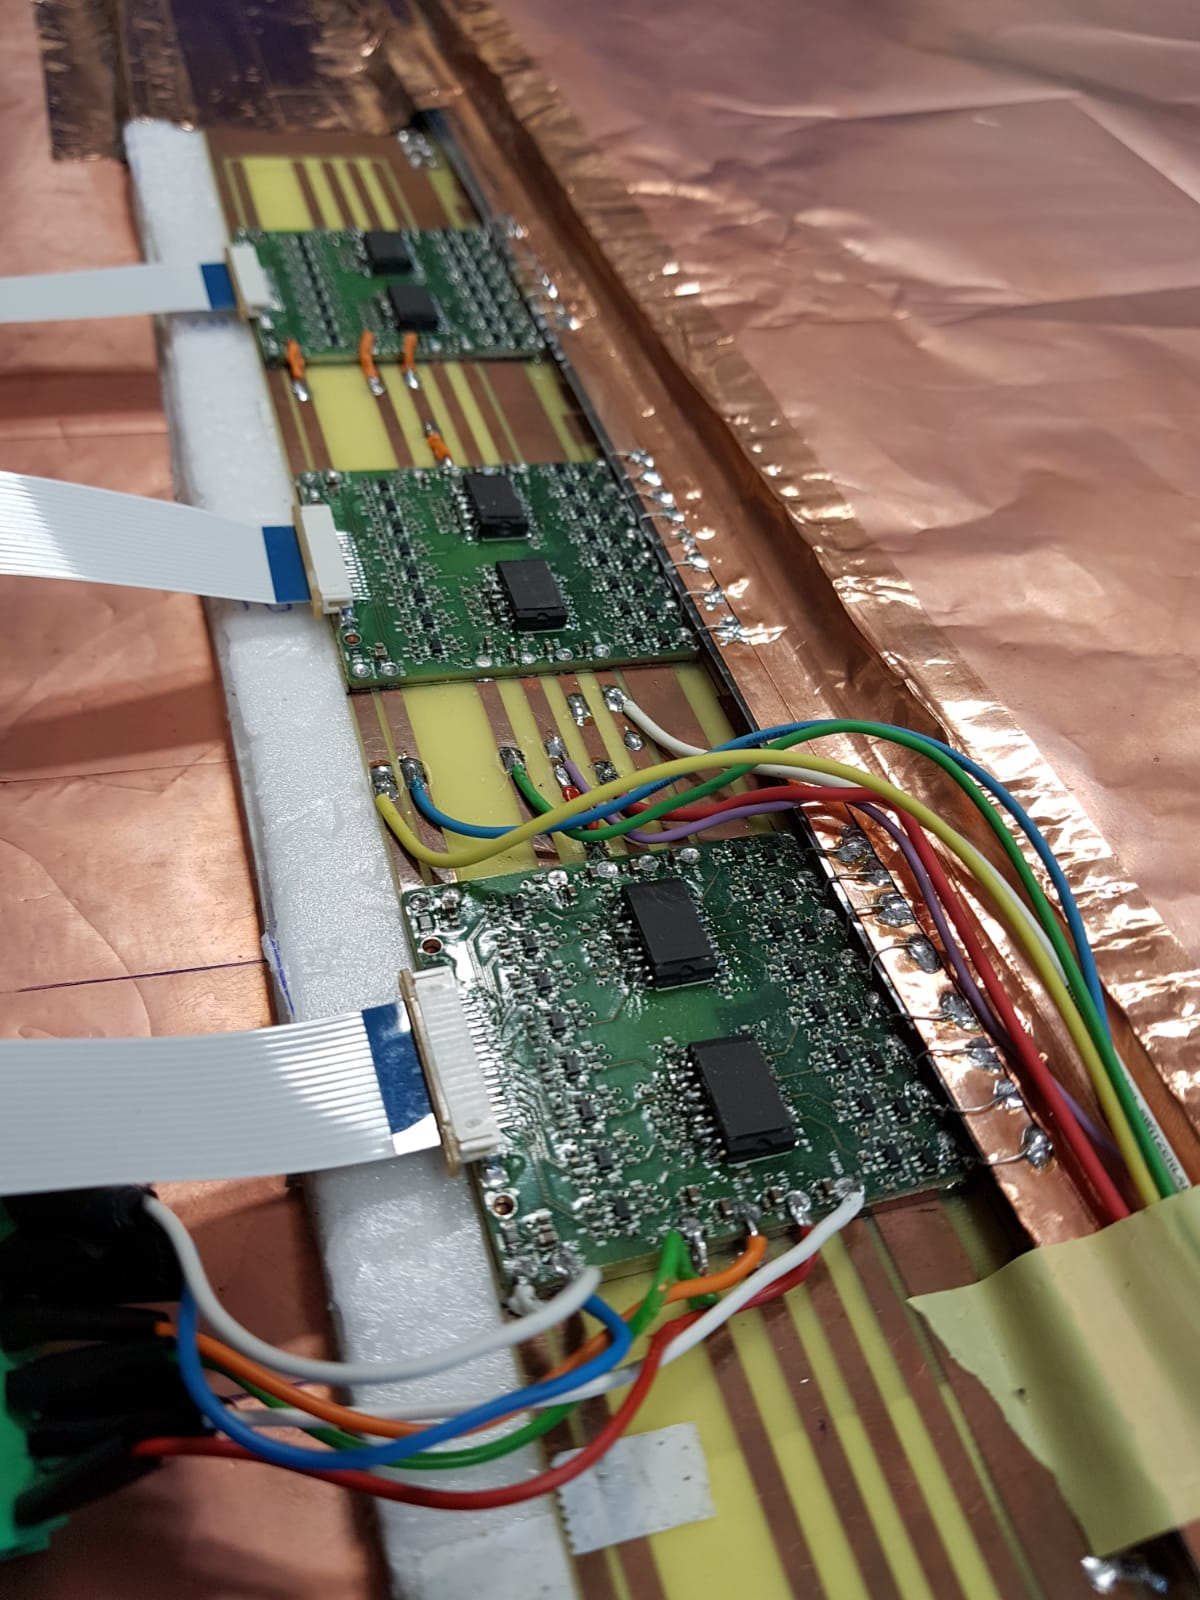
\includegraphics[height = 6cm]{fig/chapt6/INFN-FEB-on-readout.png}
			\caption{\label{fig:INFN_FEBv2:B}}
		\end{subfigure}
		\caption{\label{fig:INFN_FEBv2} Version 2 of the INFN Tor Vergata FEB as designed for the CMS iRPC. The FEBs are directly soldered onto the read-out PCB to reduce pick-up noise as much as possible. Copper lines embedded into the PCB are used to propagate the power and slow control lines.}
    \end{figure}
    
    The strips begin much wider in the case of the transversal read-out panel, the FEB design is a little different, as can be seen in Figure~\ref{fig:INFN_FEB_Trans:A}. The transversal FEBs are strictly the same as the one attached to the longitudinal plane even though they are wider. AS of now, the connection of the FEBs to the power and slow control lines is done via coaxial cables as can be seen from Figure~\ref{fig:INFN_FEB_Trans:B}. Only the connection to the strips was optimized for direct on-PCB soldering.
	 
	\begin{figure}[H]
		\begin{subfigure}{\linewidth}
		    \centering
			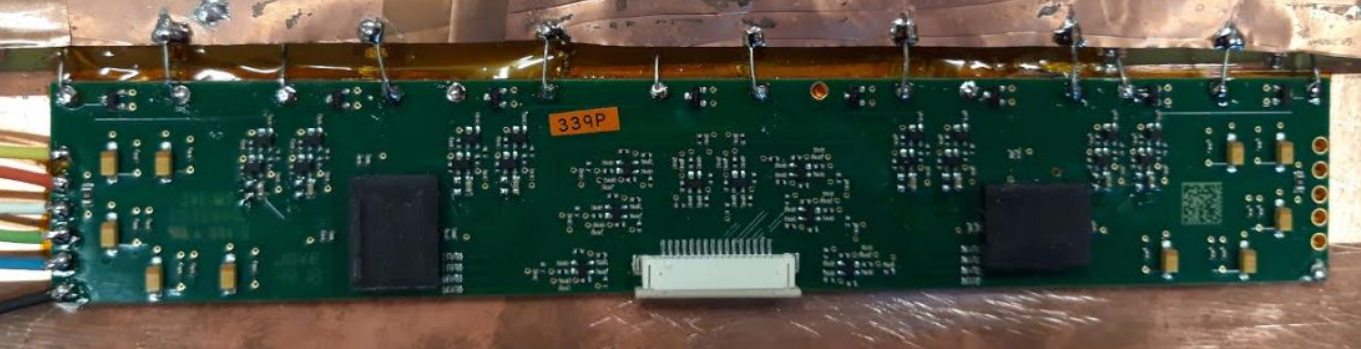
\includegraphics[width = .75\linewidth]{fig/chapt6/INFN-FEB-Transverse.png}
			\caption{\label{fig:INFN_FEB_Trans:A}}
		\end{subfigure}
		\begin{subfigure}{\linewidth}
		    \centering
			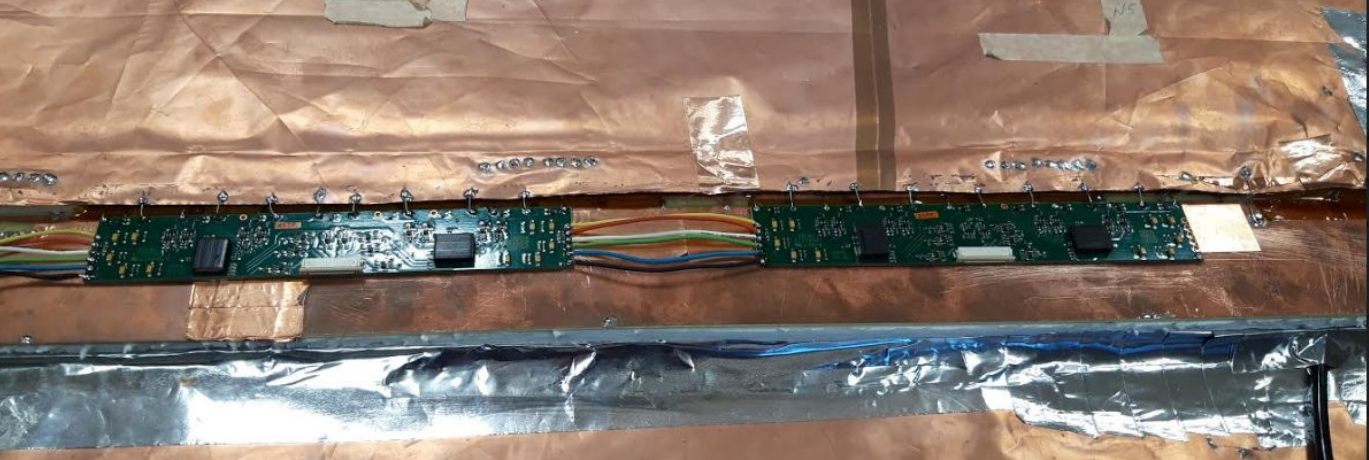
\includegraphics[width = .75\linewidth]{fig/chapt6/INFN-FEB-Transverse-on-readout.png}
			\caption{\label{fig:INFN_FEB_Trans:B}}
		\end{subfigure}
		\caption{\label{fig:INFN_FEB_Trans} Version of the INFN Tor Vergata FEB as designed for the transversal readout panels of the CMS iRPC. The FEBs are directly soldered onto the read-out PCB to reduce pick-up noise as much as possible. The propagation of the power and slow control lines is done via coaxial cables.}
    \end{figure}

\section{Preliminary electronics tests at CERN}
\label{chapt6:sec:Preliminary}

	The quest for more sensitive and low noise electronics for iRPCs started with the test of two technologies. Facing the same issue, the ATLAS collaboration at INFN Tor Vergata started developing low-noise sensitive preamplifiers to be used with RPCs. The test of these electronics was carried out by both the ATLAS and the CMS collaborations. At the same time, the \acf{IPNL} had been working on the development of an RPC based \acl{SDHCAL} for the ILD, the multi-purpose detector that is foreseen to be built at the \acf{ILC}. The RPCs they used were operated with low-noise electronics that had previously been used for timing applications with silicon photomultipliers.\\
	Both FEEs have been tested with spare CMS RPCs and \acl{gRPCs} designed and assembled in Ghent. The design of the gRPCs was derived from the gRPCs used for the SDHCAL. The were used to test the feasibility of achieving large detection areas by gluing together smaller electrodes.

	\subsection{INFN preamplifiers as upgrade candidates}
	\label{chapt6:ssec:INFN-Prelim}
	
\begingroup\setlength{\intextsep}{5pt}\setlength{\columnsep}{15pt}
	
	\begin{wrapfigure}{O}{.6\linewidth}
		\centering
		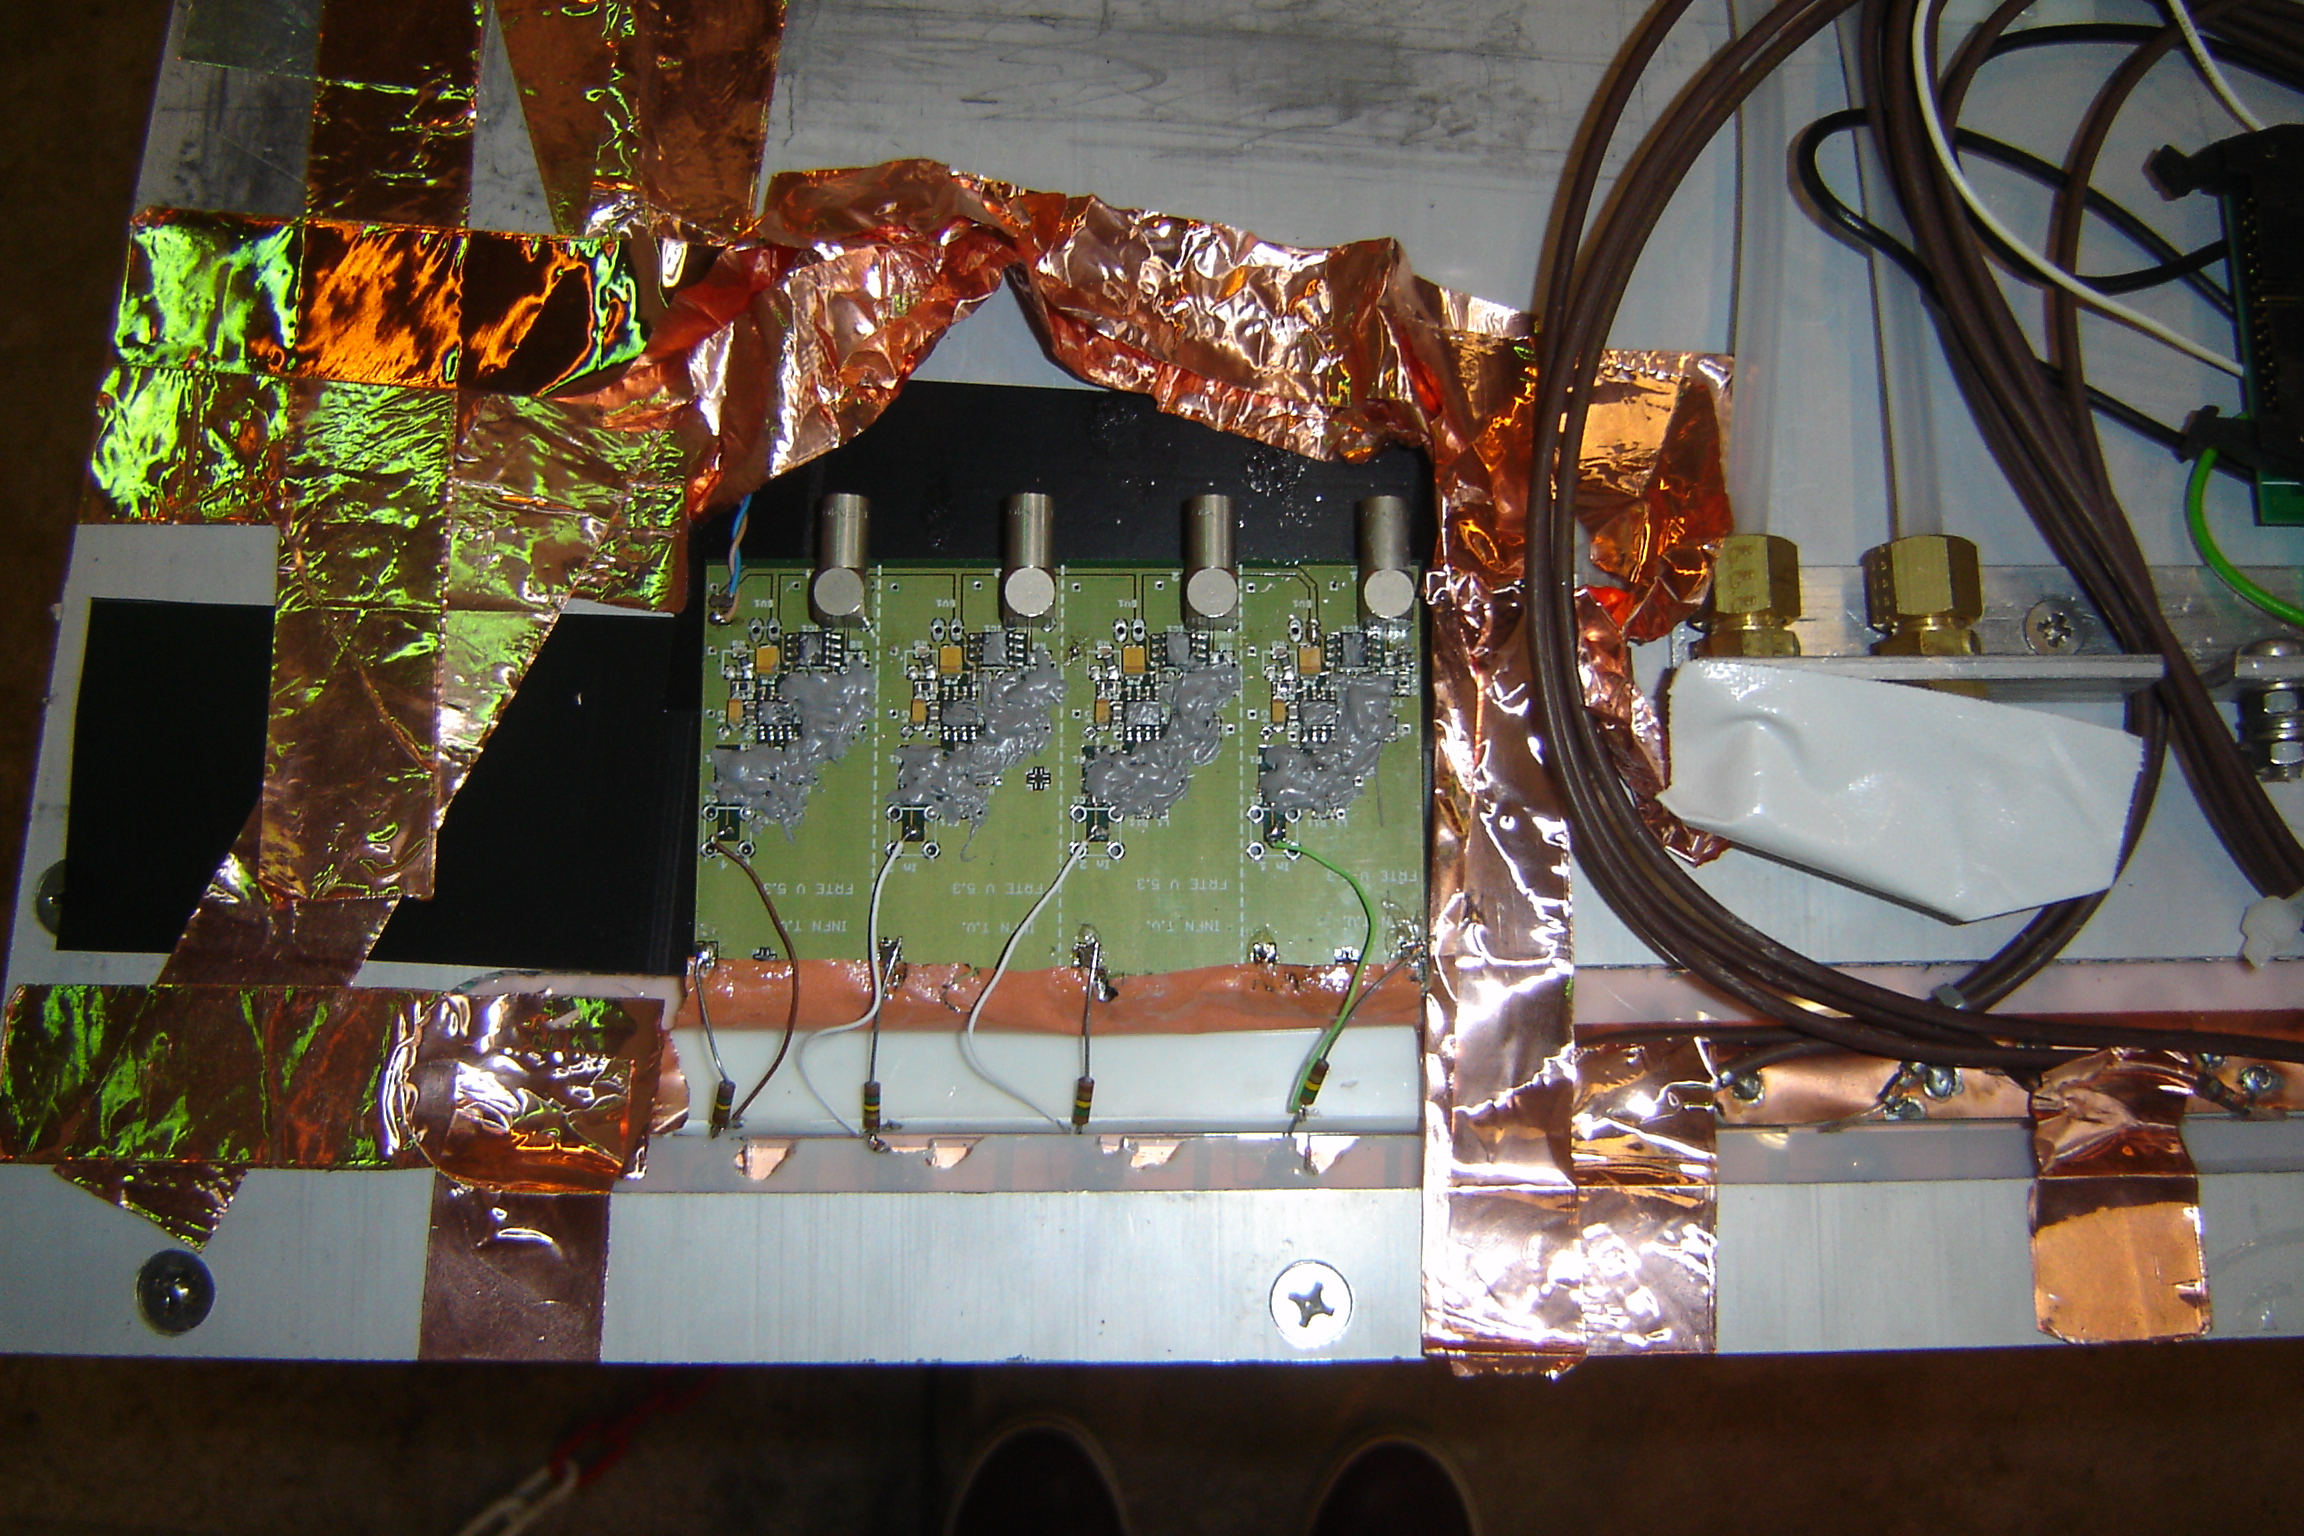
\includegraphics[width=\linewidth]{fig/chapt6/INFN-Preamp-2013.JPG}
		\caption{\label{fig:INFN-preamp} The four channels of INFN preamplifiers are mounted directly on a CMS RPC and connected to the four outermost read-out strips of the detector.}
	\end{wrapfigure}
	
	INFN electronics were the first ones to be tested by CMS RPC group in collaboration with colleagues from INFN Tor Vergata working in the ATLAS RPC group. The tests with CMS RPCs were performed in February 2013 outside of the old GIF facility presented in Chapter~\ref{chapt5:ssec:GIF}. Four preamplifier channels were lent by Cardarelli to equip four CMS RPC channels as presented in Figure~\ref{fig:INFN-preamp}. They were directly connected to the strips for the signals induced by muons passing through the gas volume of the chamber to be amplified. The output was then sent to a discriminator to digitize the signals and filter out the noise by tuning the threshold level. The NIM quad discriminator 821 manufactured by LECROY used during this experiment only allows at minimum to set the threshold at a voltage of approximately \SI{30}{mV} on the input signals. Thus, two values of discrimination were used ($\sim$\SI{75}{mV} and $\sim$\SI{30}{mV}).
	
\endgroup
	
	The performance of the chamber equipped with these new preamplifiers was compared to the performance of CMS FEEs. The experimental setup used is described in Figure~\ref{fig:Setup-GIF}. PMTs a little less wide than four strips were used to trigger the data tacking. Two pairs were used in coincidence on both the strips connected to the INFN preamplifiers and to the ones connected to the CMS FEEs. An extra PMT, placed perpendicularly to the rest of the setup at the bottom of the setup was used to detect potential showers and send VETO signals if necessary. A last PMT was used close to the power supplies to measure and discard signals due to electromagnetic noise and is not visible on the pictures. Finally, after discrimination, the output of the INFN preamplifiers together with the signals from the CMS FEEs were sent to scalers to count the detected signals versus the number of trigger coincidences as no DAQ software was available at the time. The full pulse processing for this experiment is shown in Figure~\ref{fig:Pulse-Processing}.
	 
	\begin{figure}[H]
		\begin{subfigure}{\linewidth}
		    \centering
			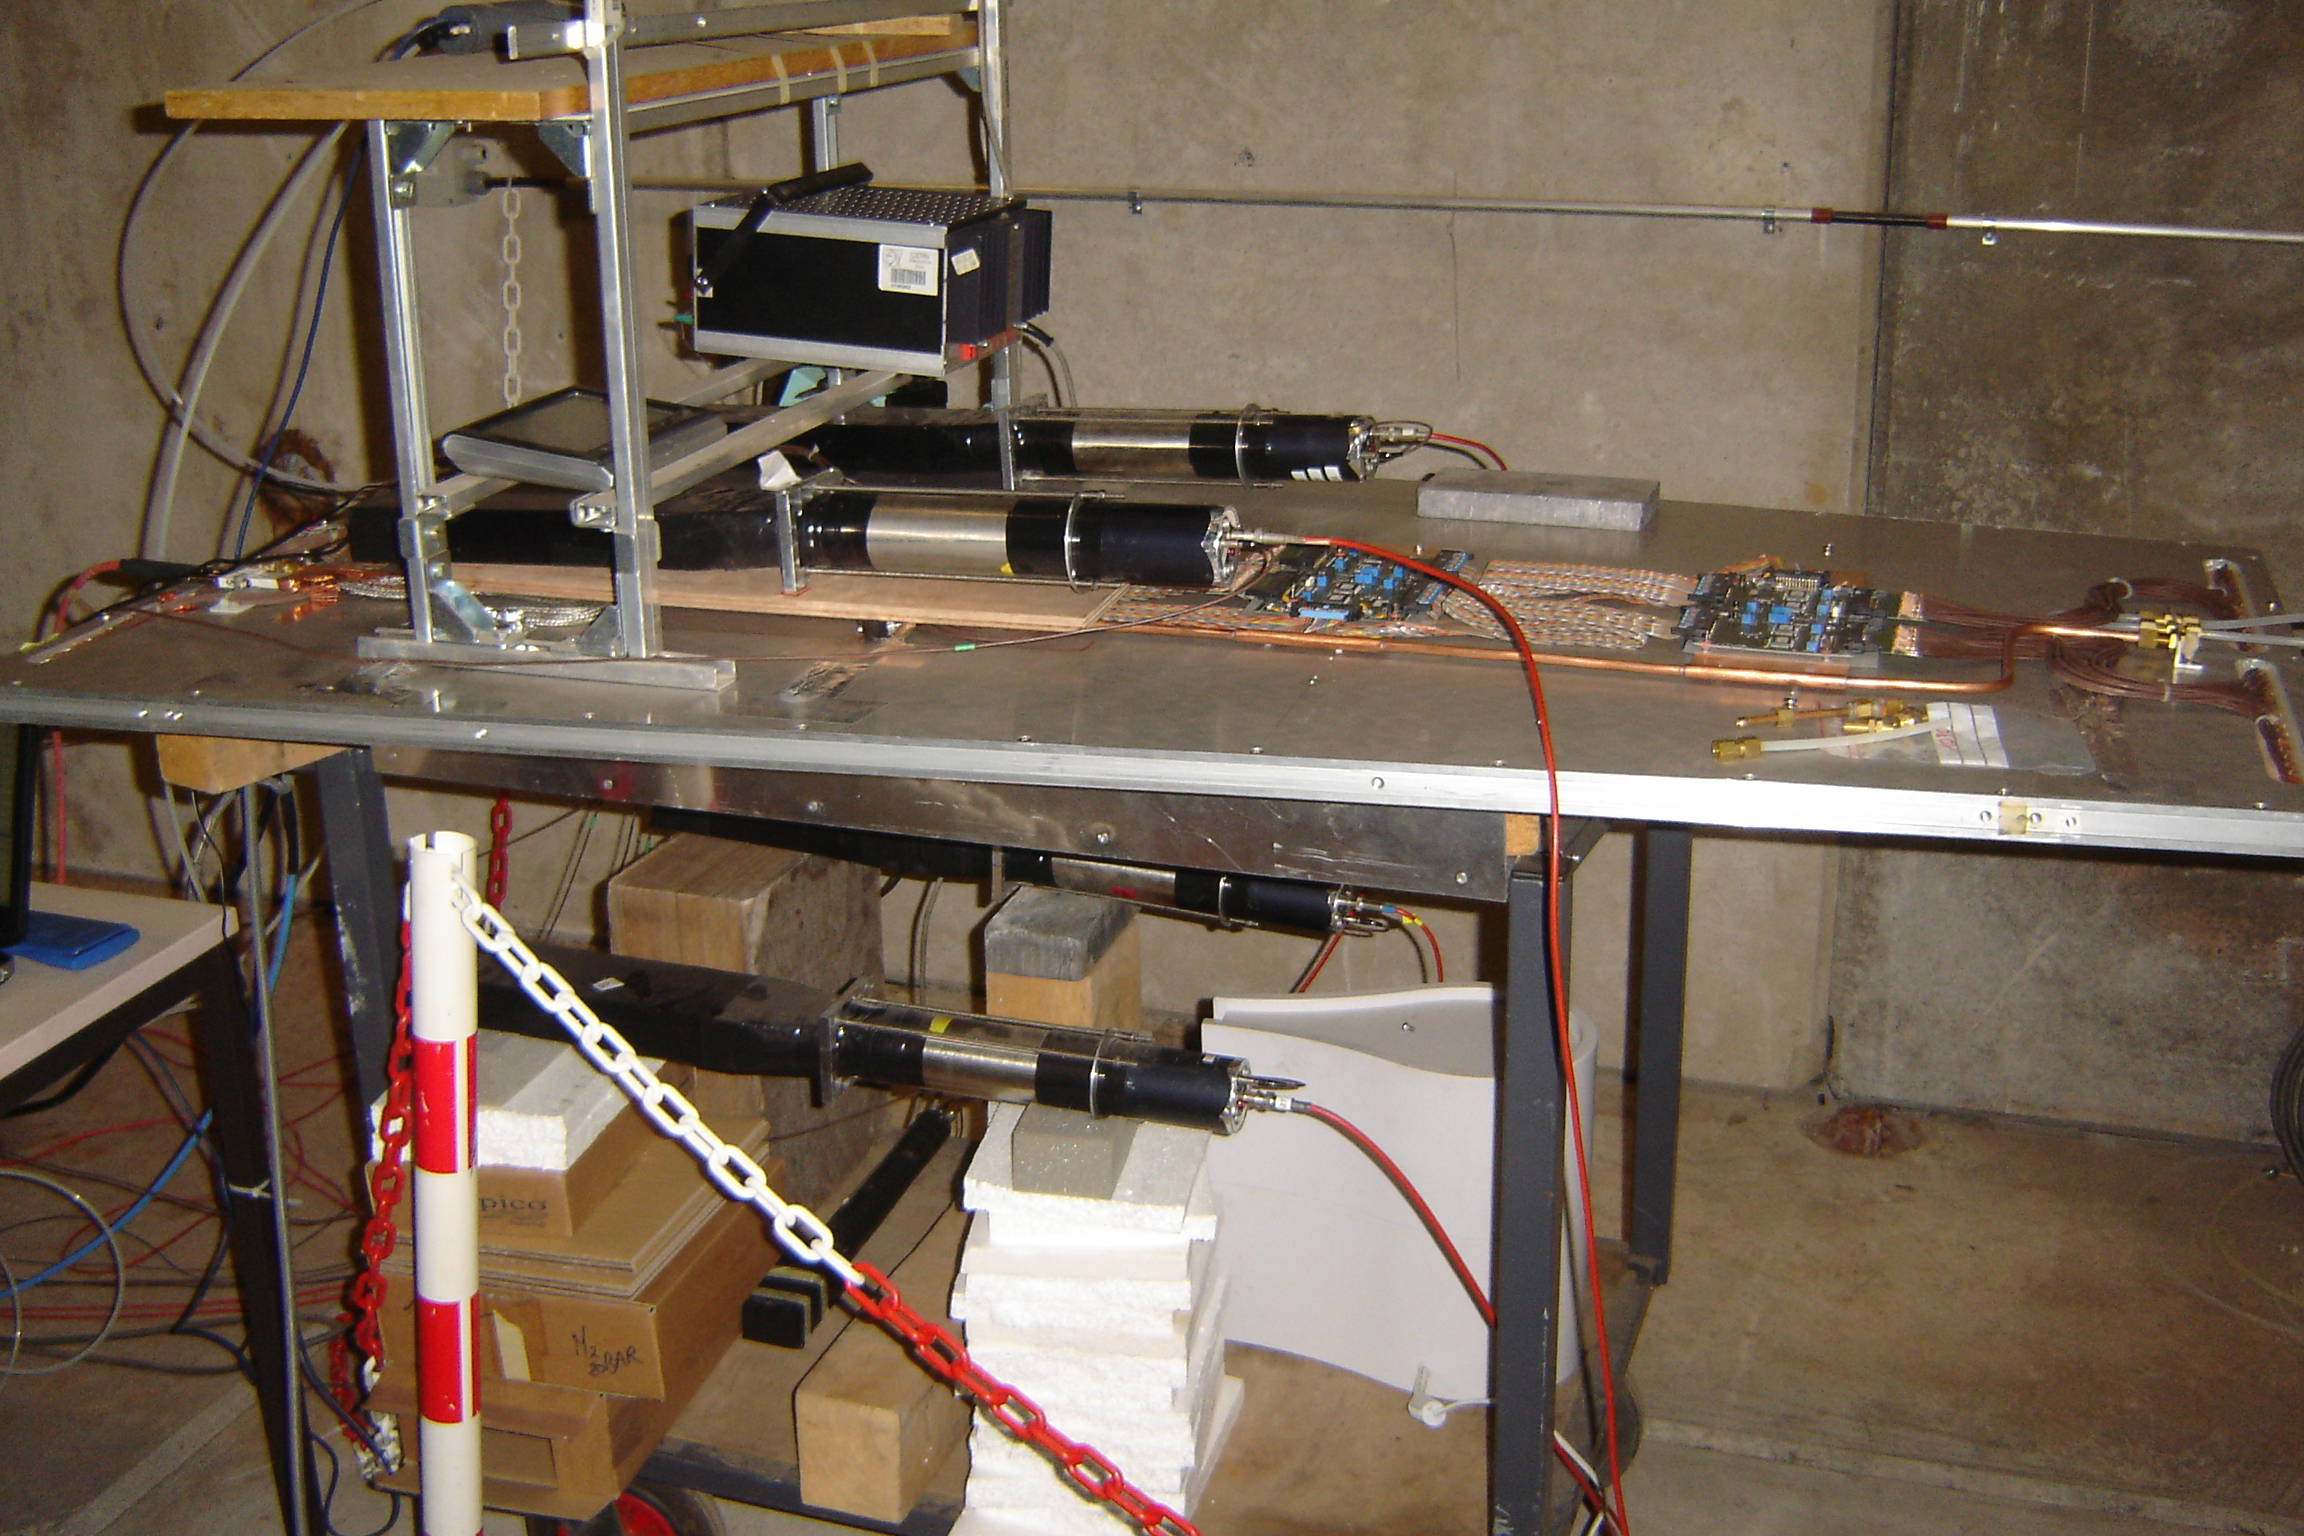
\includegraphics[width = 0.7\linewidth]{fig/chapt6/Setup-GIF-side.JPG}
			\caption{\label{fig:Setup-GIF:A}}
		\end{subfigure}
		\begin{subfigure}{0.5\linewidth}
		    \centering
			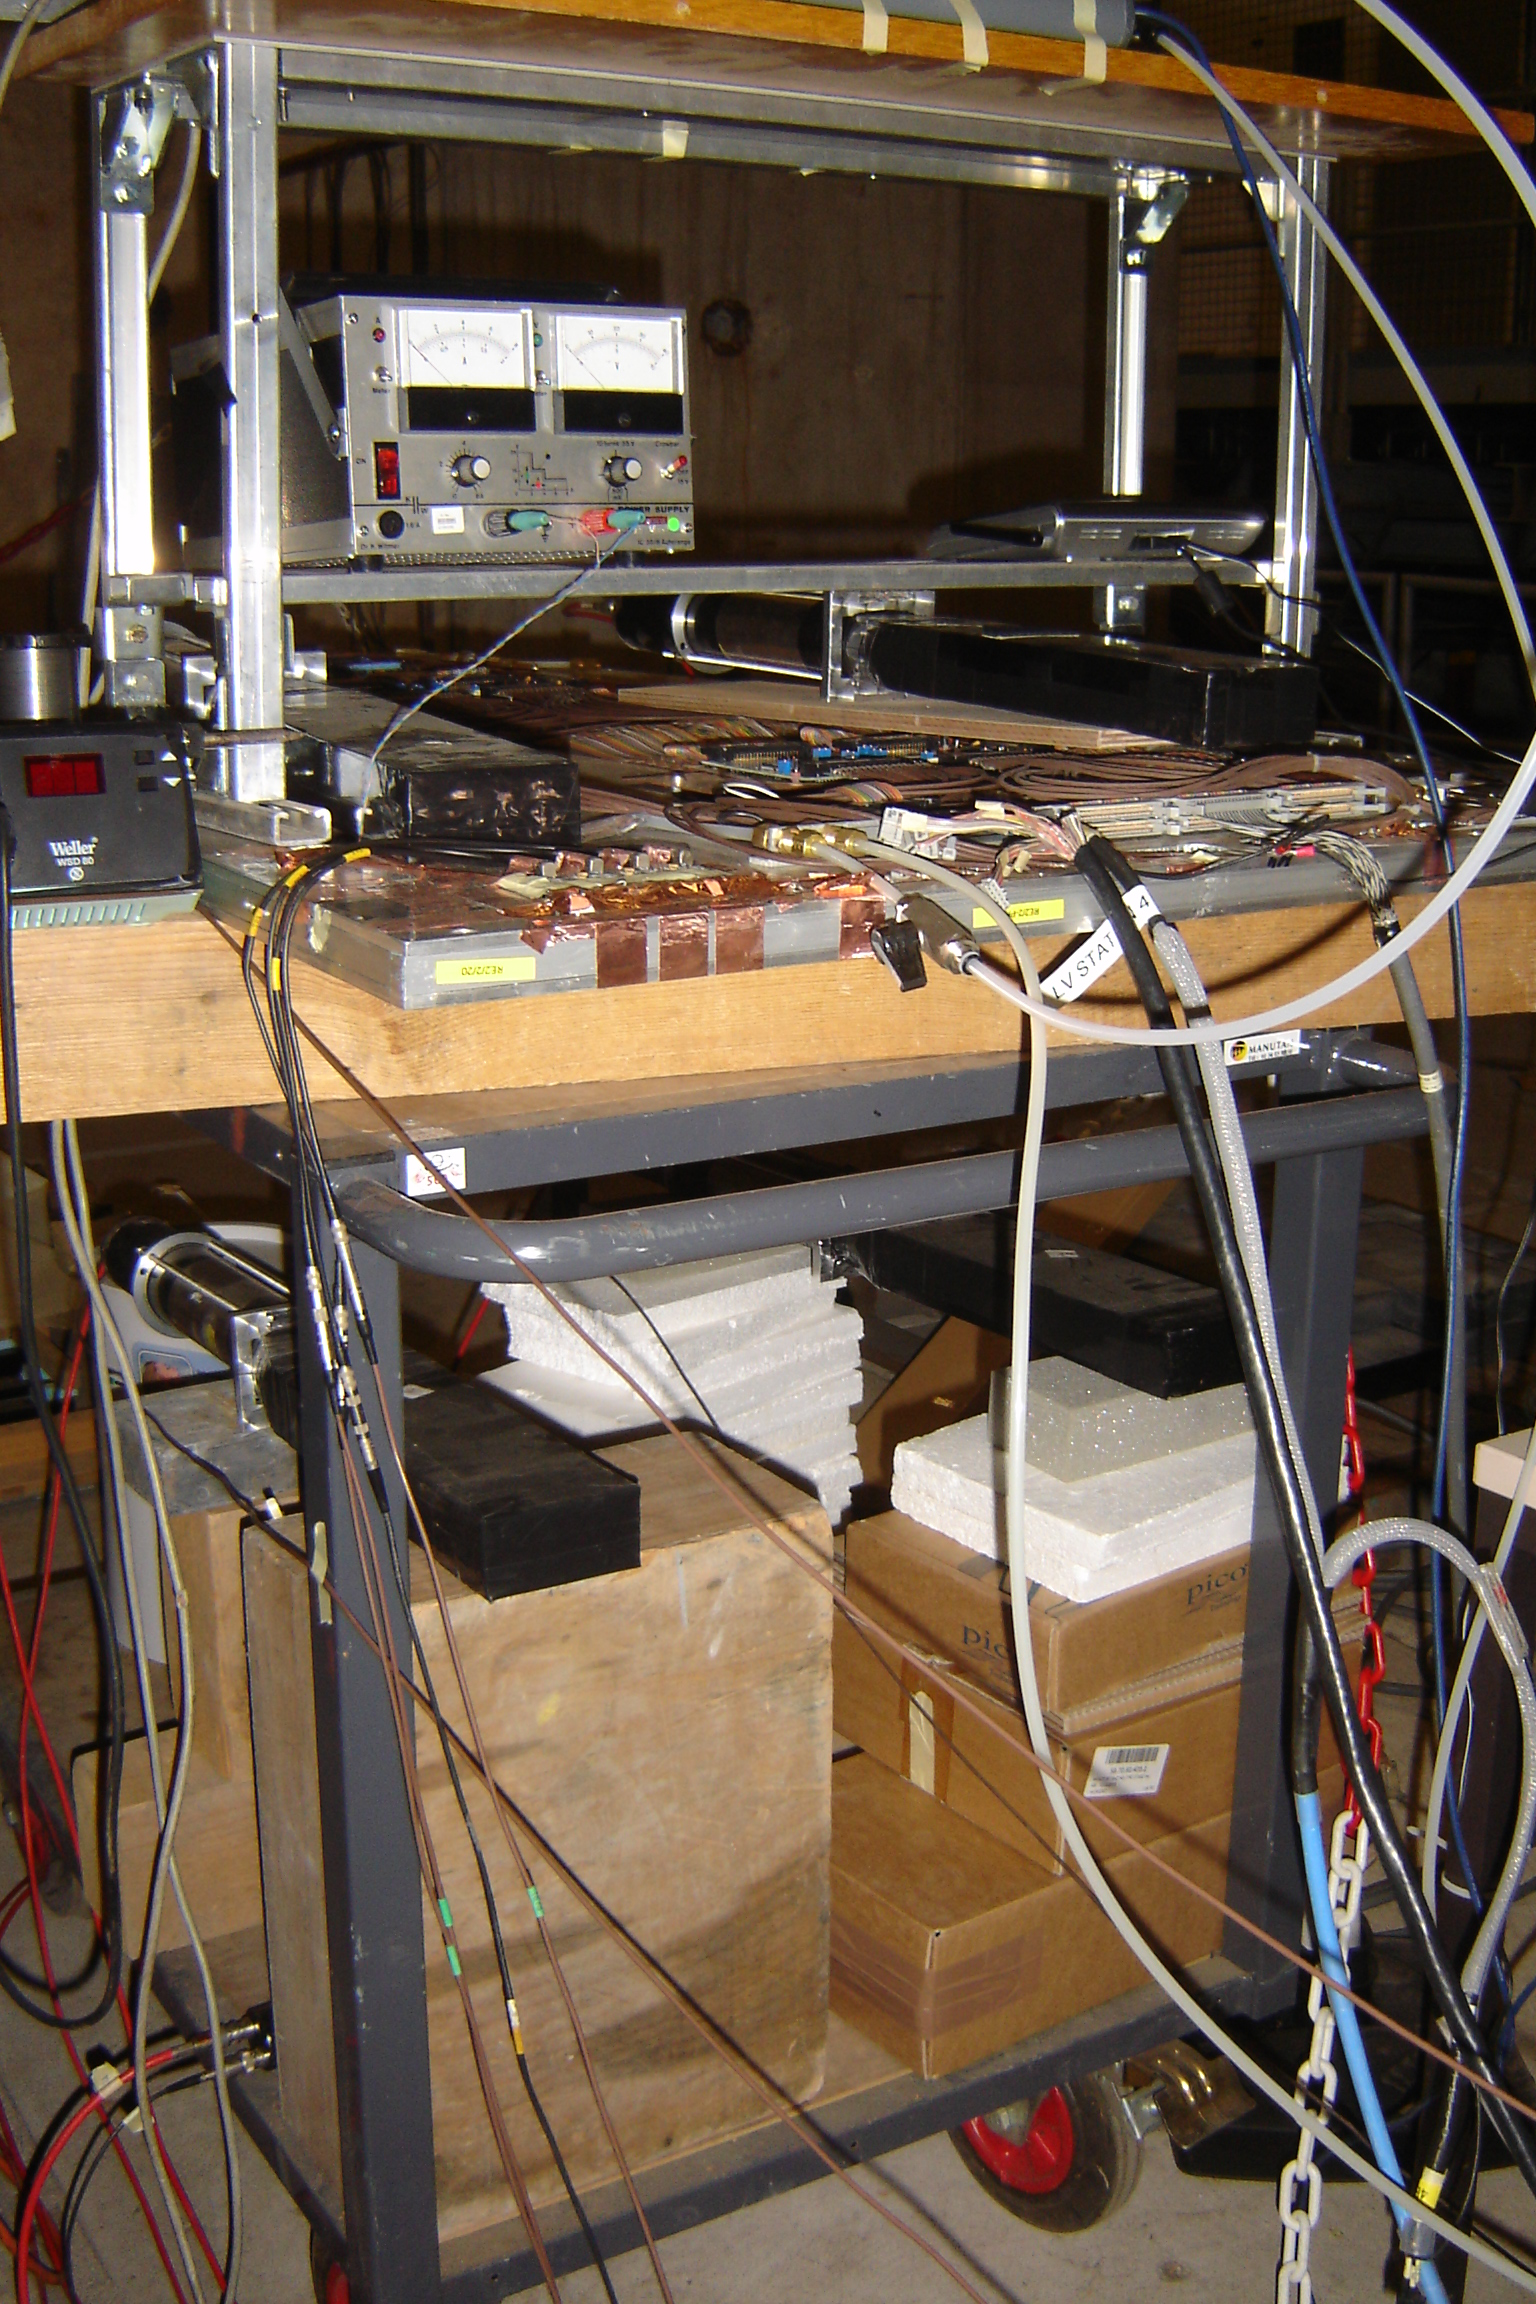
\includegraphics[width = 0.9\linewidth]{fig/chapt6/Setup-GIF-front.JPG}
			\caption{\label{fig:Setup-GIF:B}}
		\end{subfigure}
		\begin{subfigure}{0.5\linewidth}
		    \centering
			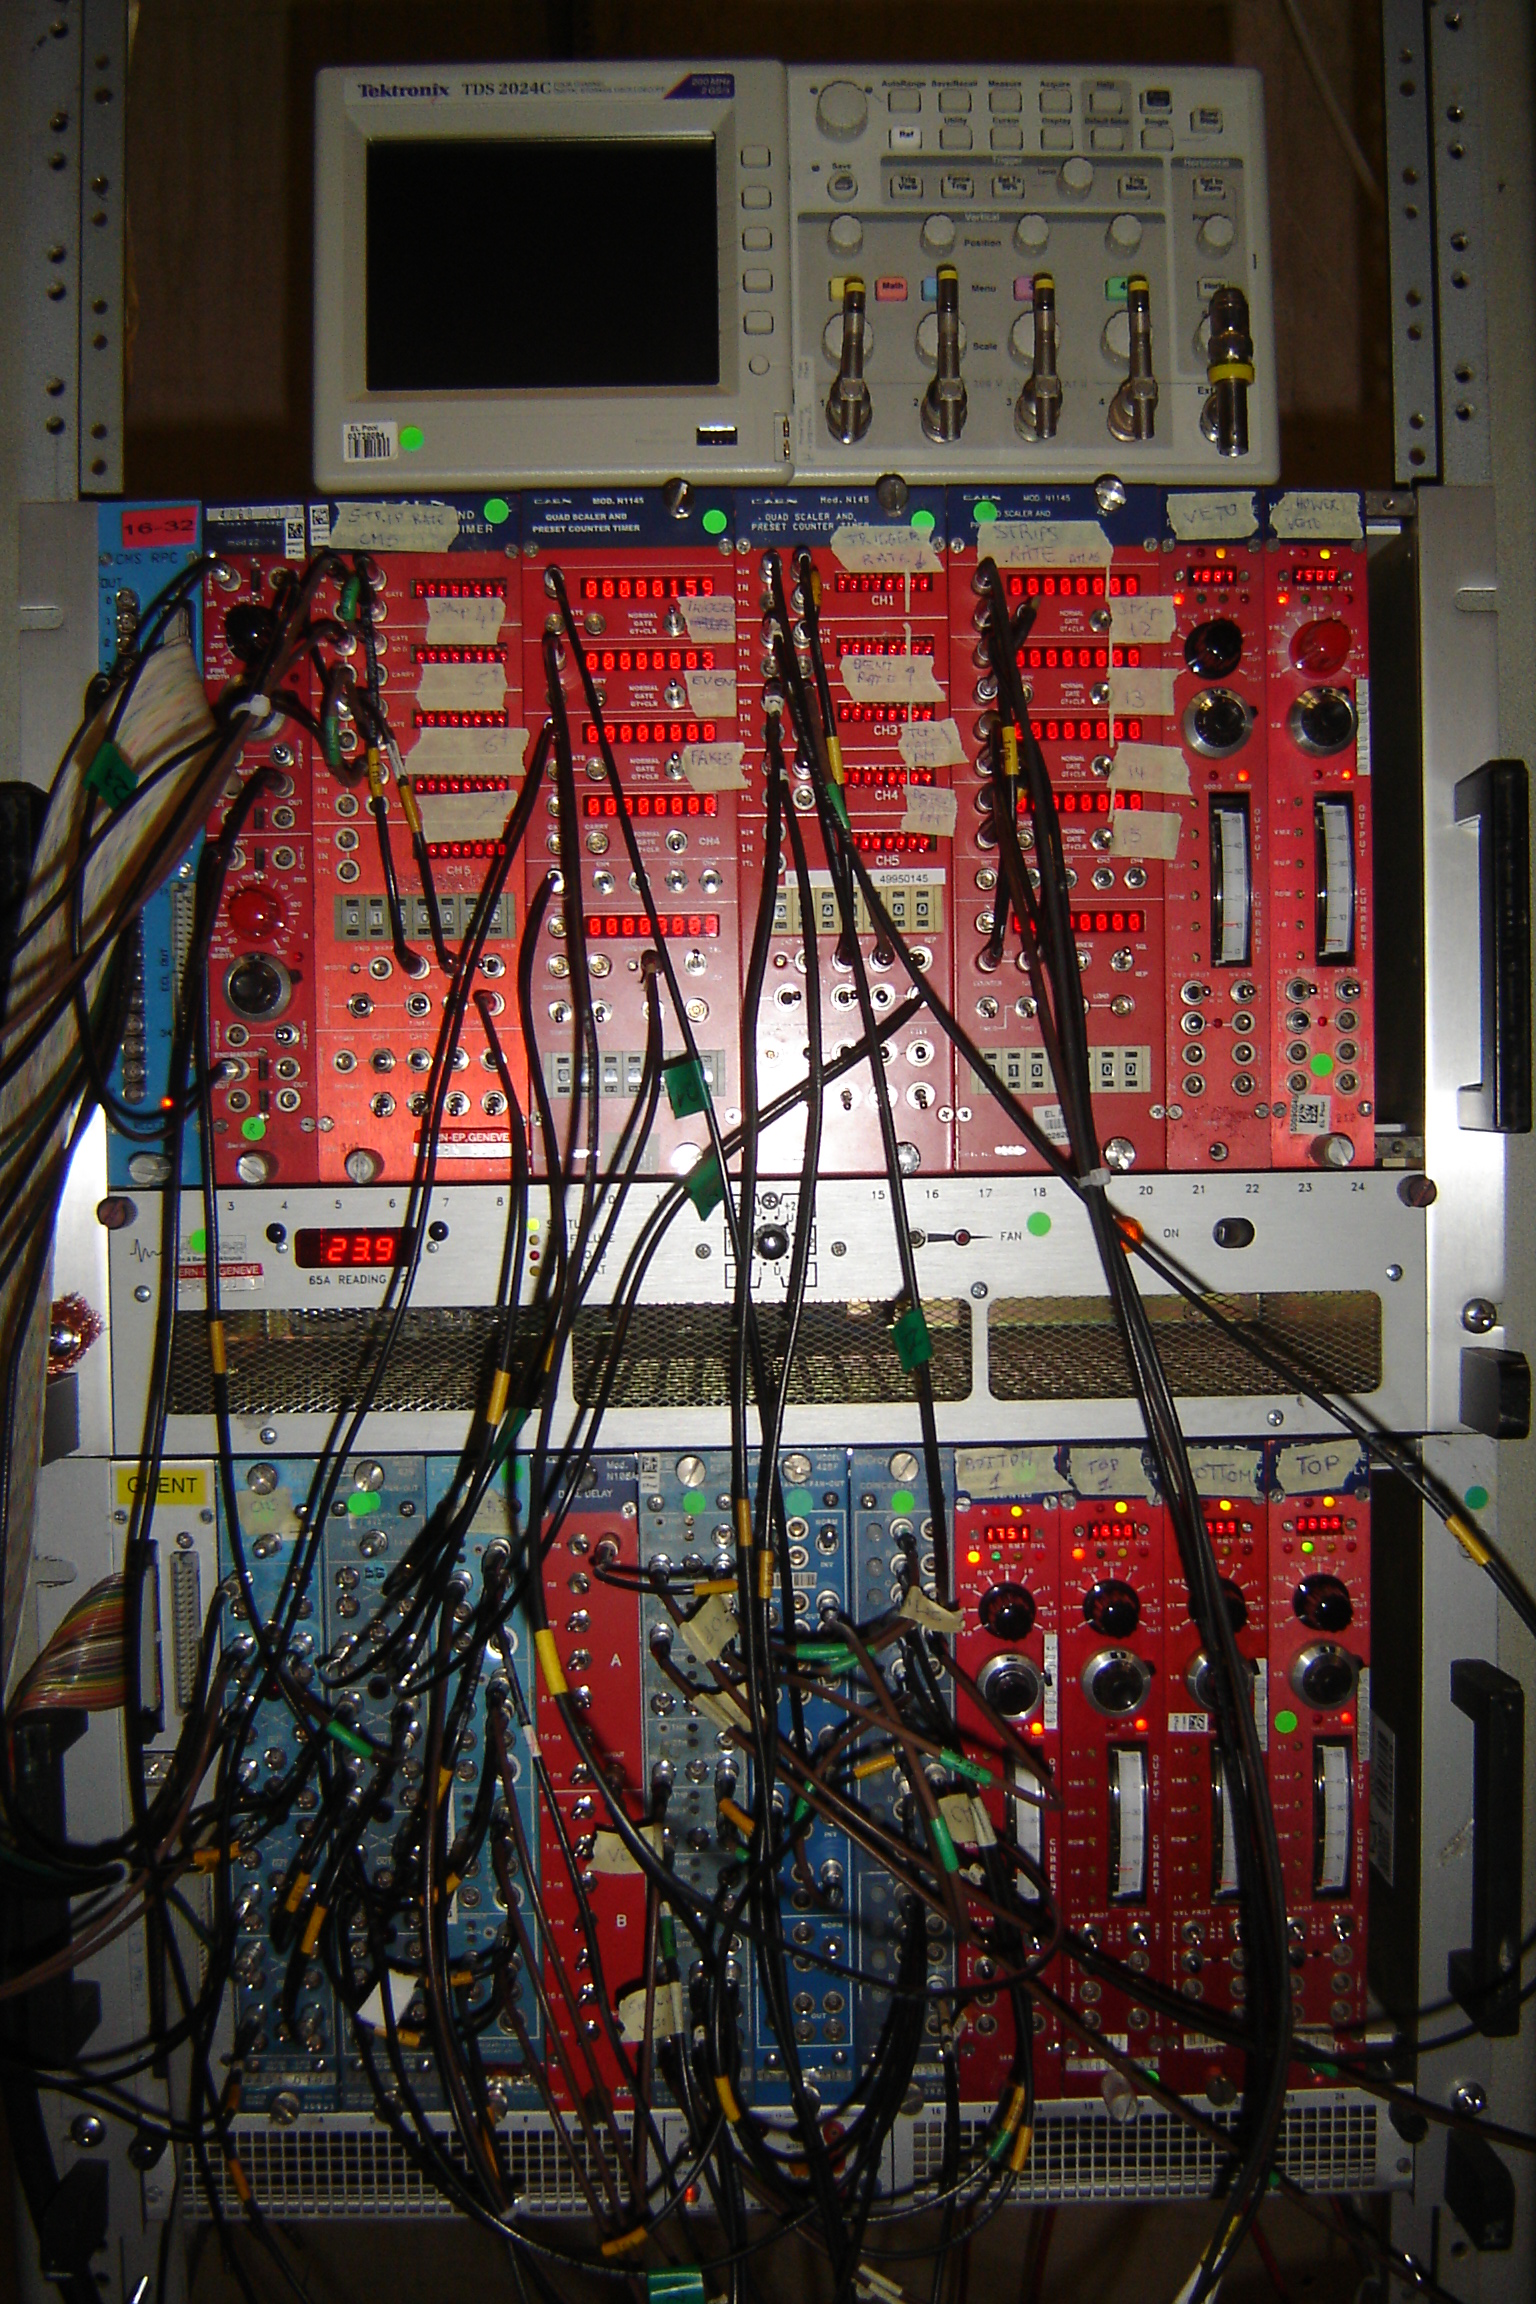
\includegraphics[width = 0.9\linewidth]{fig/chapt6/Pulse-processing-GIF.JPG}
			\caption{\label{fig:Setup-GIF:C}}
		\end{subfigure}
		\caption{\label{fig:Setup-GIF} Experimental setup used to test the INFN preamplifier with respect to the CMS FEEs.}
    \end{figure}
	 
	\begin{figure}[H]
		\begin{subfigure}{.5\linewidth}
		    \centering
			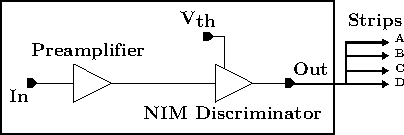
\includegraphics[width = 0.9\linewidth]{fig/chapt6/atlas-block-diagram-2013.pdf}
			\caption{\label{fig:Pulse-Processing:A}}
		\end{subfigure}
		\begin{subfigure}{.5\linewidth}
		    \centering
			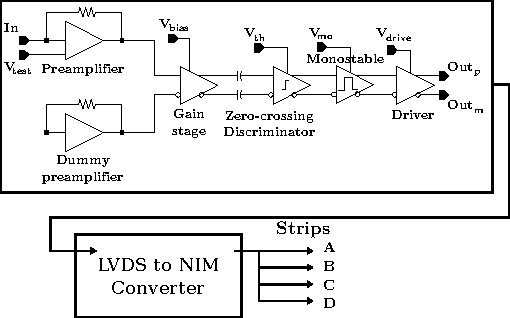
\includegraphics[width = 0.9\linewidth]{fig/chapt6/cms-block-diagram-2013.pdf}
			\caption{\label{fig:Pulse-Processing:B}}
		\end{subfigure}
		\begin{subfigure}{\linewidth}
		    \centering
			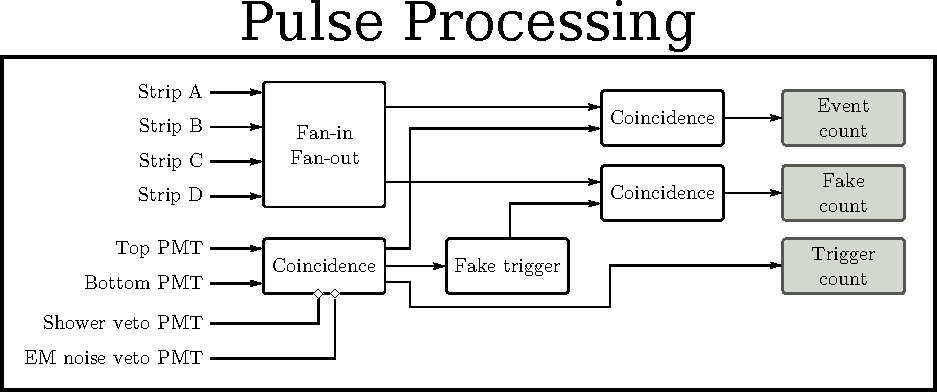
\includegraphics[width = 0.8\linewidth]{fig/chapt6/pulse-processing-2013.pdf}
			\caption{\label{fig:Pulse-Processing:C}}
		\end{subfigure}
		\caption{\label{fig:Pulse-Processing} The block diagrams corresponding to the signal treatment for both INFN preamplifier~\subref{fig:Pulse-Processing:A} and CMS FEEs~\subref{fig:Pulse-Processing:B} are shown. The digitized signals are then counted in coincidence with the trigger signals provided by PMTs~\subref{fig:Pulse-Processing:C}.}
    \end{figure}
    
	The data taking program consisted in \acl{HV} scans. A first point was taken at \SI{0}{V} to only measure noise. Then the HV was increased to an applied value of \SI{7}{kV}. The voltage was increased in steps of \SI{500}{V} until \SI{8}{kV} from where it was increased in steps of \SI{100}{V} until an upper limit of \SI{10}{kV}. After rising the voltage over the electrodes of the RPC, a waiting period of 15 minutes was observed to leave time to the electrodes to charge and to the currents to stabilize. The currents were reported at the moment the data taking was started. At each HV step, except at \SI{0}{V}, approximatively 300 triggers were taken to estimate the efficiency of the detector by counting the number of hits in the system (A or B or C or D), referring to the strips. The noise rate per unit area was measured during the first \SI{100}{s} of data taking by counting the number of hits received in each read-out strip. The cluster size, the average number of adjacent strips fired during a muon event, could not be measured due to the lack of available scalers.\\
	During the data acquisition, in addition to counting the number of signals with respect to the number of triggers, the current or the noise rate per unit area as a function of the increasing voltage, the environmental parameters were monitored. Using the information provided by a humidity and temperature sensor on the gas input line together with the environmental pressure given by a weather station, the applied voltage could be corrected following Formula~\ref{eq:PTCMS}. Moreover, the voltage line was filtered to prevent noise and higher currents in the RPC under test.
    
	The results of the preliminary tests are presented in Figure~\ref{fig:INFN-preamp-res}. More details on the fit performed on the data are provided in Table~\ref{tab:INFN-preamp}. As can be seen, being able to use electronics with a much higher sensitivity allows for an HV shift of up to \SI{475}{V} with a threshold as low as \SI{3}{fC} corresponding to the lowest threshold available on the discriminator modules. On the other hand, the higher charge sensitivity also brings a higher noise level. After a first series of measurement performed with a bad grounding leading to grounding loops and hence an artificially higher noise, it can be concluded that the noise rate per unit area of such electronics is approximately one order of magnitude higher than the noise rate measured with the CMS FEB. The noise reaches approximately \SIrate{2} at the level of the working in the case of the INFN preamplifier while it is lower than \SIrate{0.2} for the CMS FEB. It is likely that the higher sensitivity also brings a higher sensitivity to local discharges happening in the gas due to fluctuations of the electric field. The surface of the electrodes being not perfectly smooth, the local electric field may vary quickly. The gas molecules circulating in the gas could then be ionised by the fast variation of the field and trigger an avalanche that can then be detected. Reducing the noise rate per unit area would then come from an improvement of the detector itself rather than from a reduction of the electronic noise of the INFN preamplifier.
	
	\begin{figure}[H]
		\begin{subfigure}{.5\linewidth}
		    \centering
			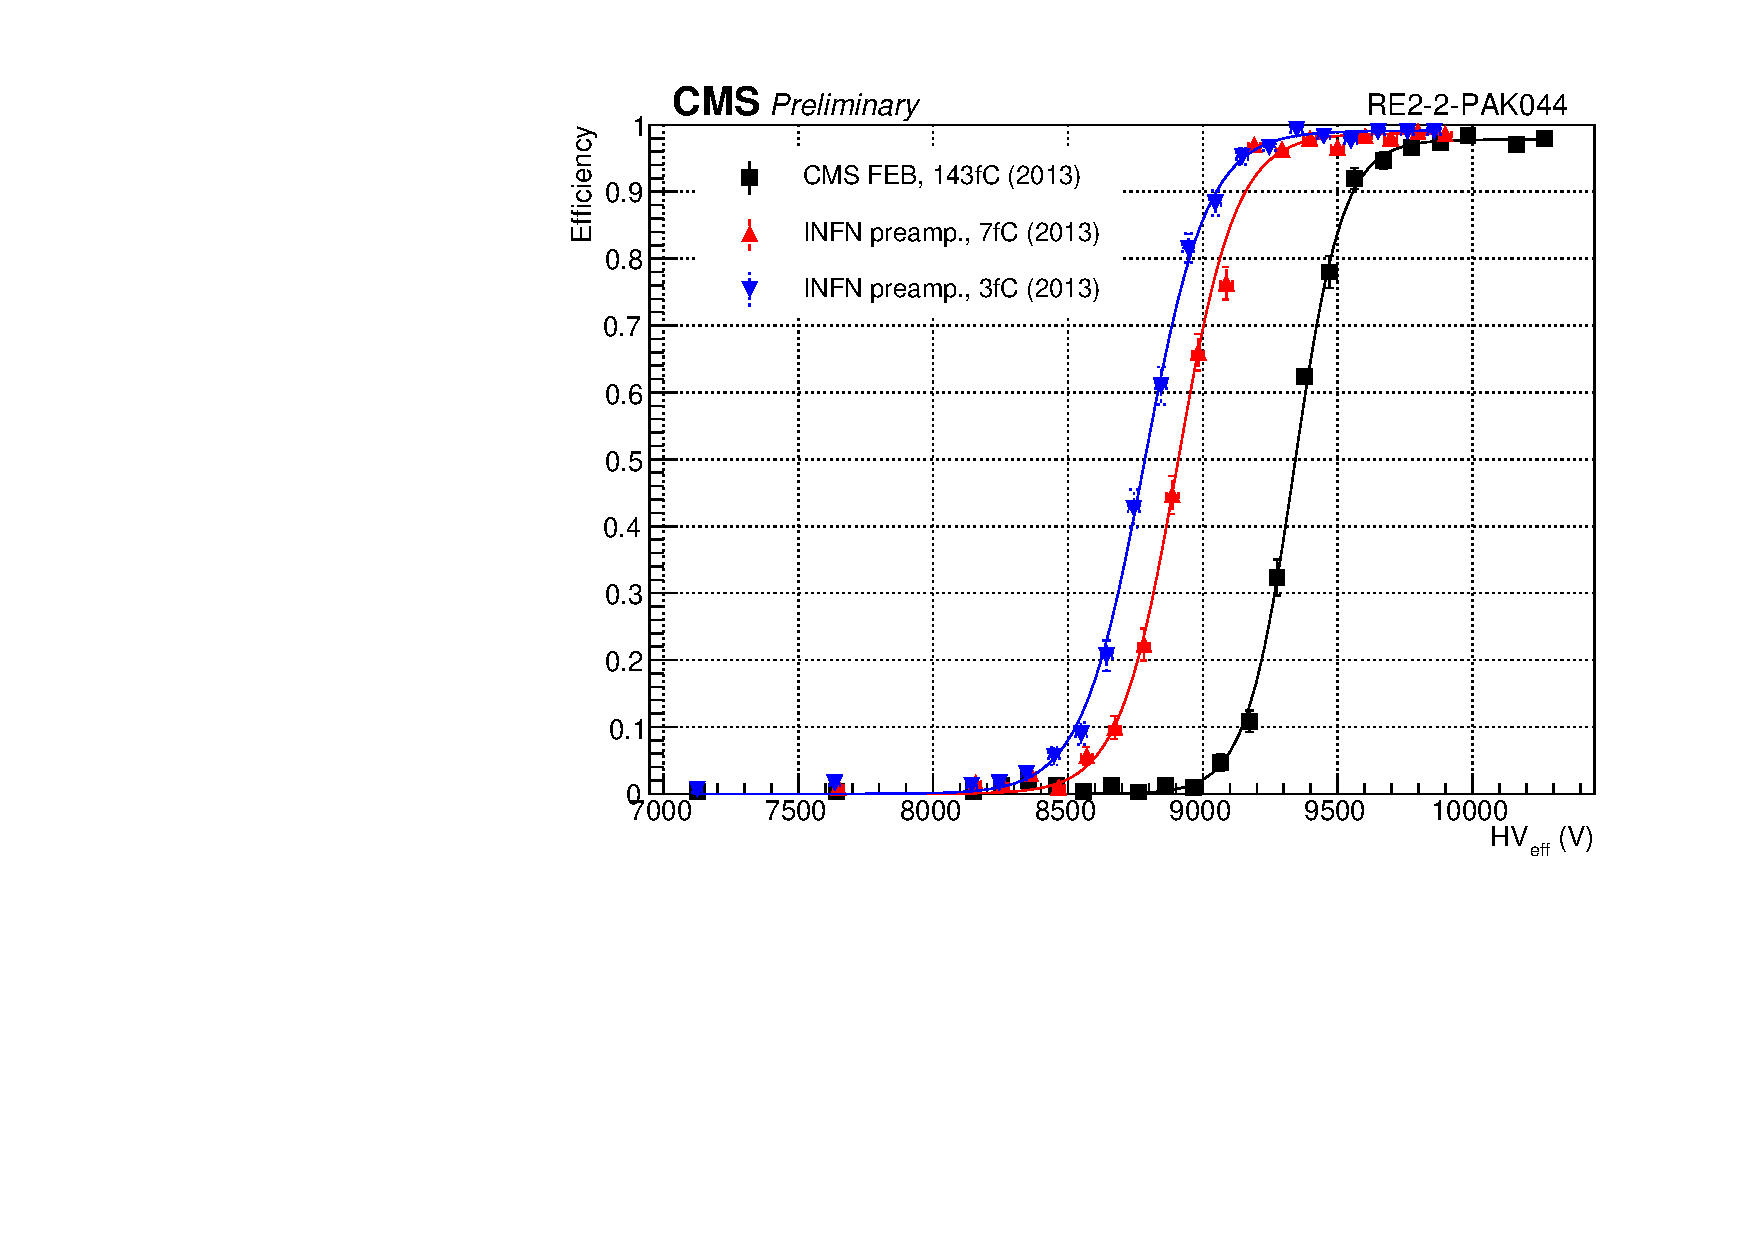
\includegraphics[width=\linewidth]{fig/chapt6/INFN-Preamplifier-Shift.pdf}
			\caption{\label{fig:INFN-preamp-res:A}}
		\end{subfigure}
		\begin{subfigure}{.5\linewidth}
		    \centering
			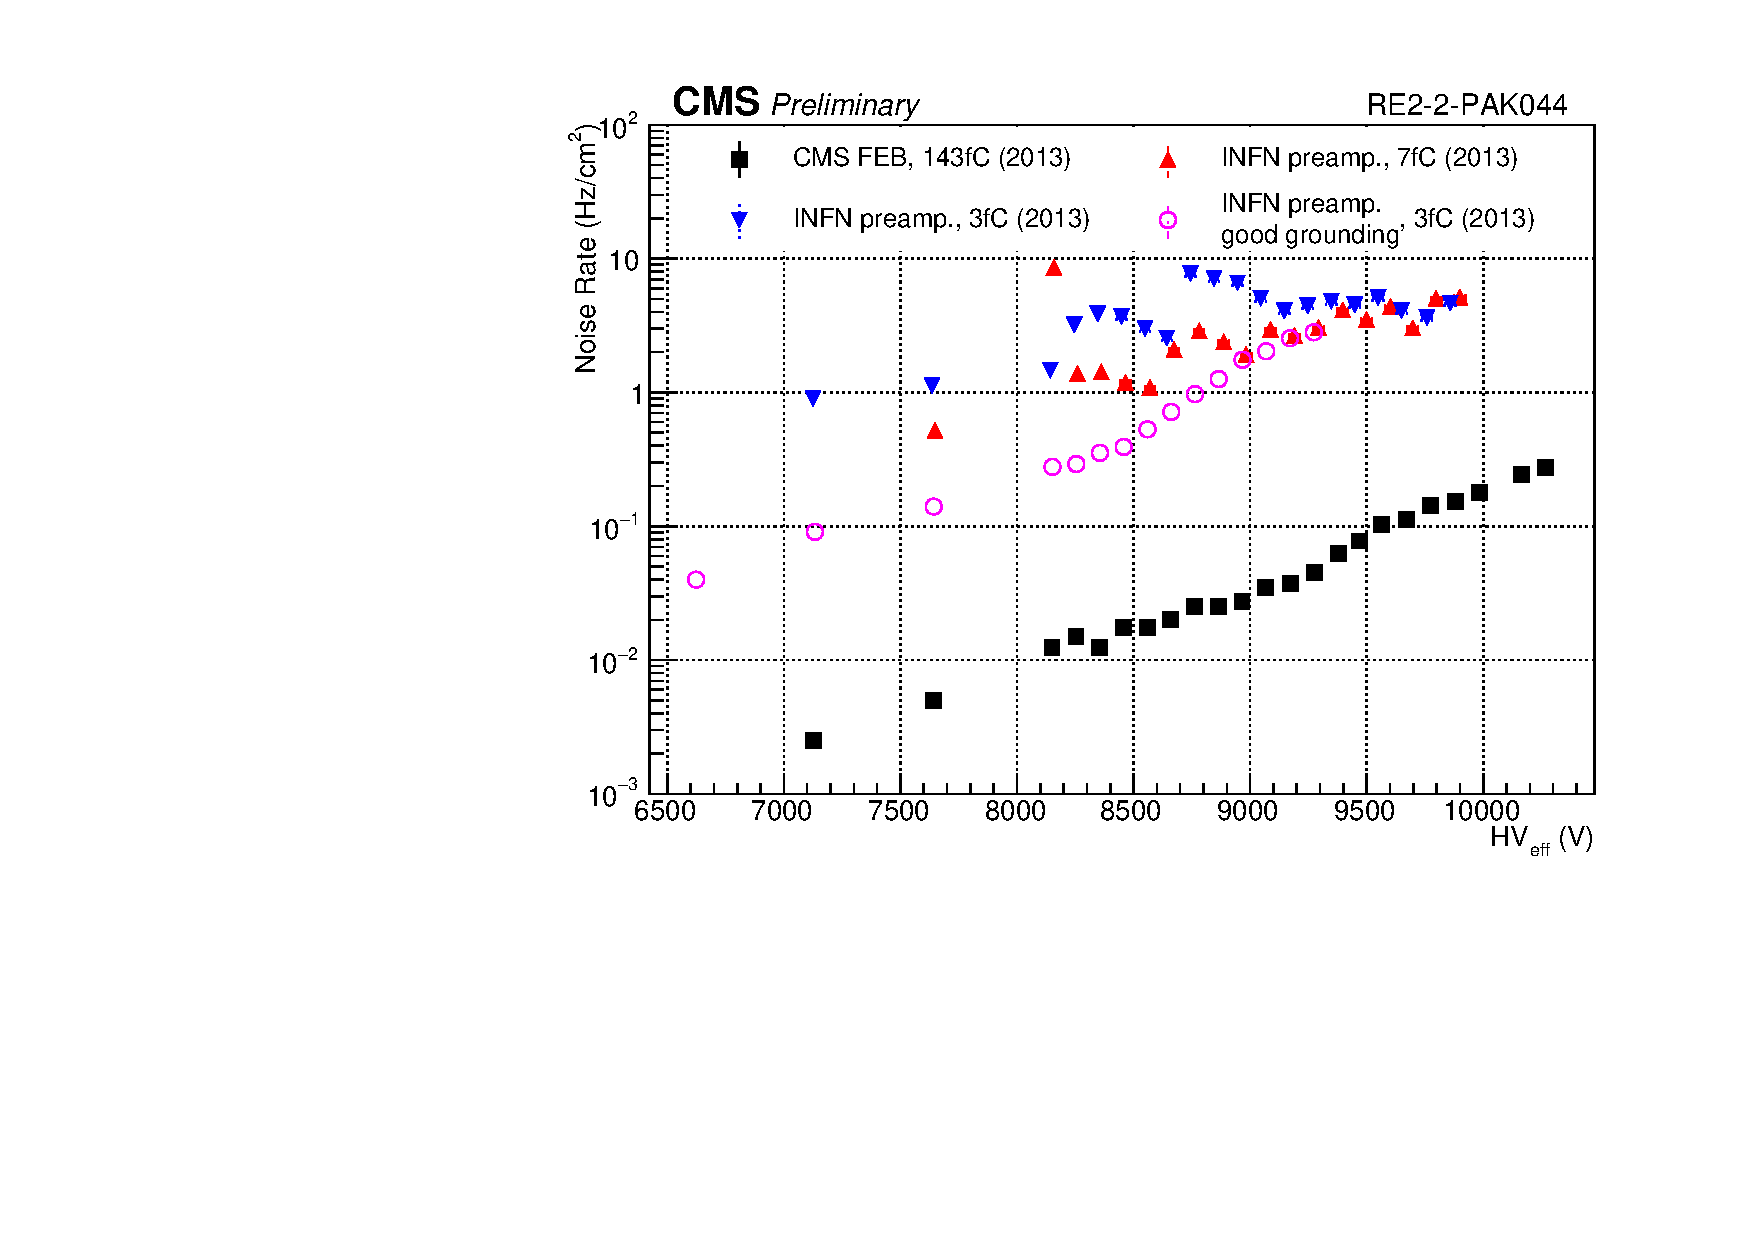
\includegraphics[width = \linewidth]{fig/chapt6/INFN-Preamplifier-Rate-Shift.pdf}
			\caption{\label{fig:INFN-preamp-res:B}}
		\end{subfigure}
		\caption{\label{fig:INFN-preamp-res} Efficiency~\subref{fig:INFN-preamp-res:A} and noise rate per unit area~\subref{fig:INFN-preamp-res:B} of the CMS RE2-2 detector tested with the standard CMS FEBs (black) and with the INFN preamplifier at different thresholds (red and blue). An extra HV scan was performed with better conditions to measure the noise with a threshold of \SI{3}{fC} on the INFN preamplifiers.}
	\end{figure}
	
	\begin{table}[H]
		\caption{\label{tab:INFN-preamp} Results of the sigmoid fit (Formula~\ref{eq:Sigmoid}) performed on the data presented in Figure~\ref{fig:INFN-preamp-res:A}. The working point and its corresponding efficiency are computed using Formulas~\ref{eq:Sigmoid} and \ref{eq:KneeWP}.}
		\footnotesize
		\begin{tabular}{|c|c|c|c|c|c|}
			\hline
Data & $\epsilon_{max}$  & $\lambda$ ($\times$\Ord{-2} \si{V^{-1}}) & $HV_{50}$ (\si{V}) & $\epsilon_{WP}$ & $HV_{WP}$ (\si{V}) \\ 
			\hline
CMS FEB, 143fC (2013)    & $0.978 \pm 0.004$ & $1.12 \pm 0.07$ & $9339 \pm 11$ & $0.97 \pm 0.01$ & $9752 \pm 27$\\ 
			\hline
INFN preamp., 7fC (2013) & $0.987 \pm 0.003$ & $0.93 \pm 0.05$ & $8907 \pm 11$ & $0.97 \pm 0.01$ & $9374 \pm 27$\\ 
			\hline
INFN preamp., 3fC (2013) & $0.991 \pm 0.003$ & $0.86 \pm 0.04$ & $8783 \pm 11$ & $0.98 \pm 0.01$ & $9276 \pm 27$\\ 
			\hline
		\end{tabular}
	\end{table}

	\subsection{INFN preamplifiers mounted onto CMS \acl{FEB}}
	\label{chapt6:ssec:INFN-FEB}
	
	Following the first experiment performed in the experimental hall aside of the old GIF, a new series of tests has been done in the CMS RPC assembly laboratory at CERN. For this purpose, the preamplifiers have been designed to be standalone single channels. To have a consistent comparison with the CMS FEB, a FEB prototype has been built based on the current CMS design. As shown in Figure~\ref{fig:Setup-INFN-904}, the preamplifiers are meant to be plugged in one of the available 16 channels of the board that produces an LVDS output with similar characteristics than the CMS FEB.
	 
	\begin{figure}[H]
		\begin{subfigure}{.6\linewidth}
		    \centering
			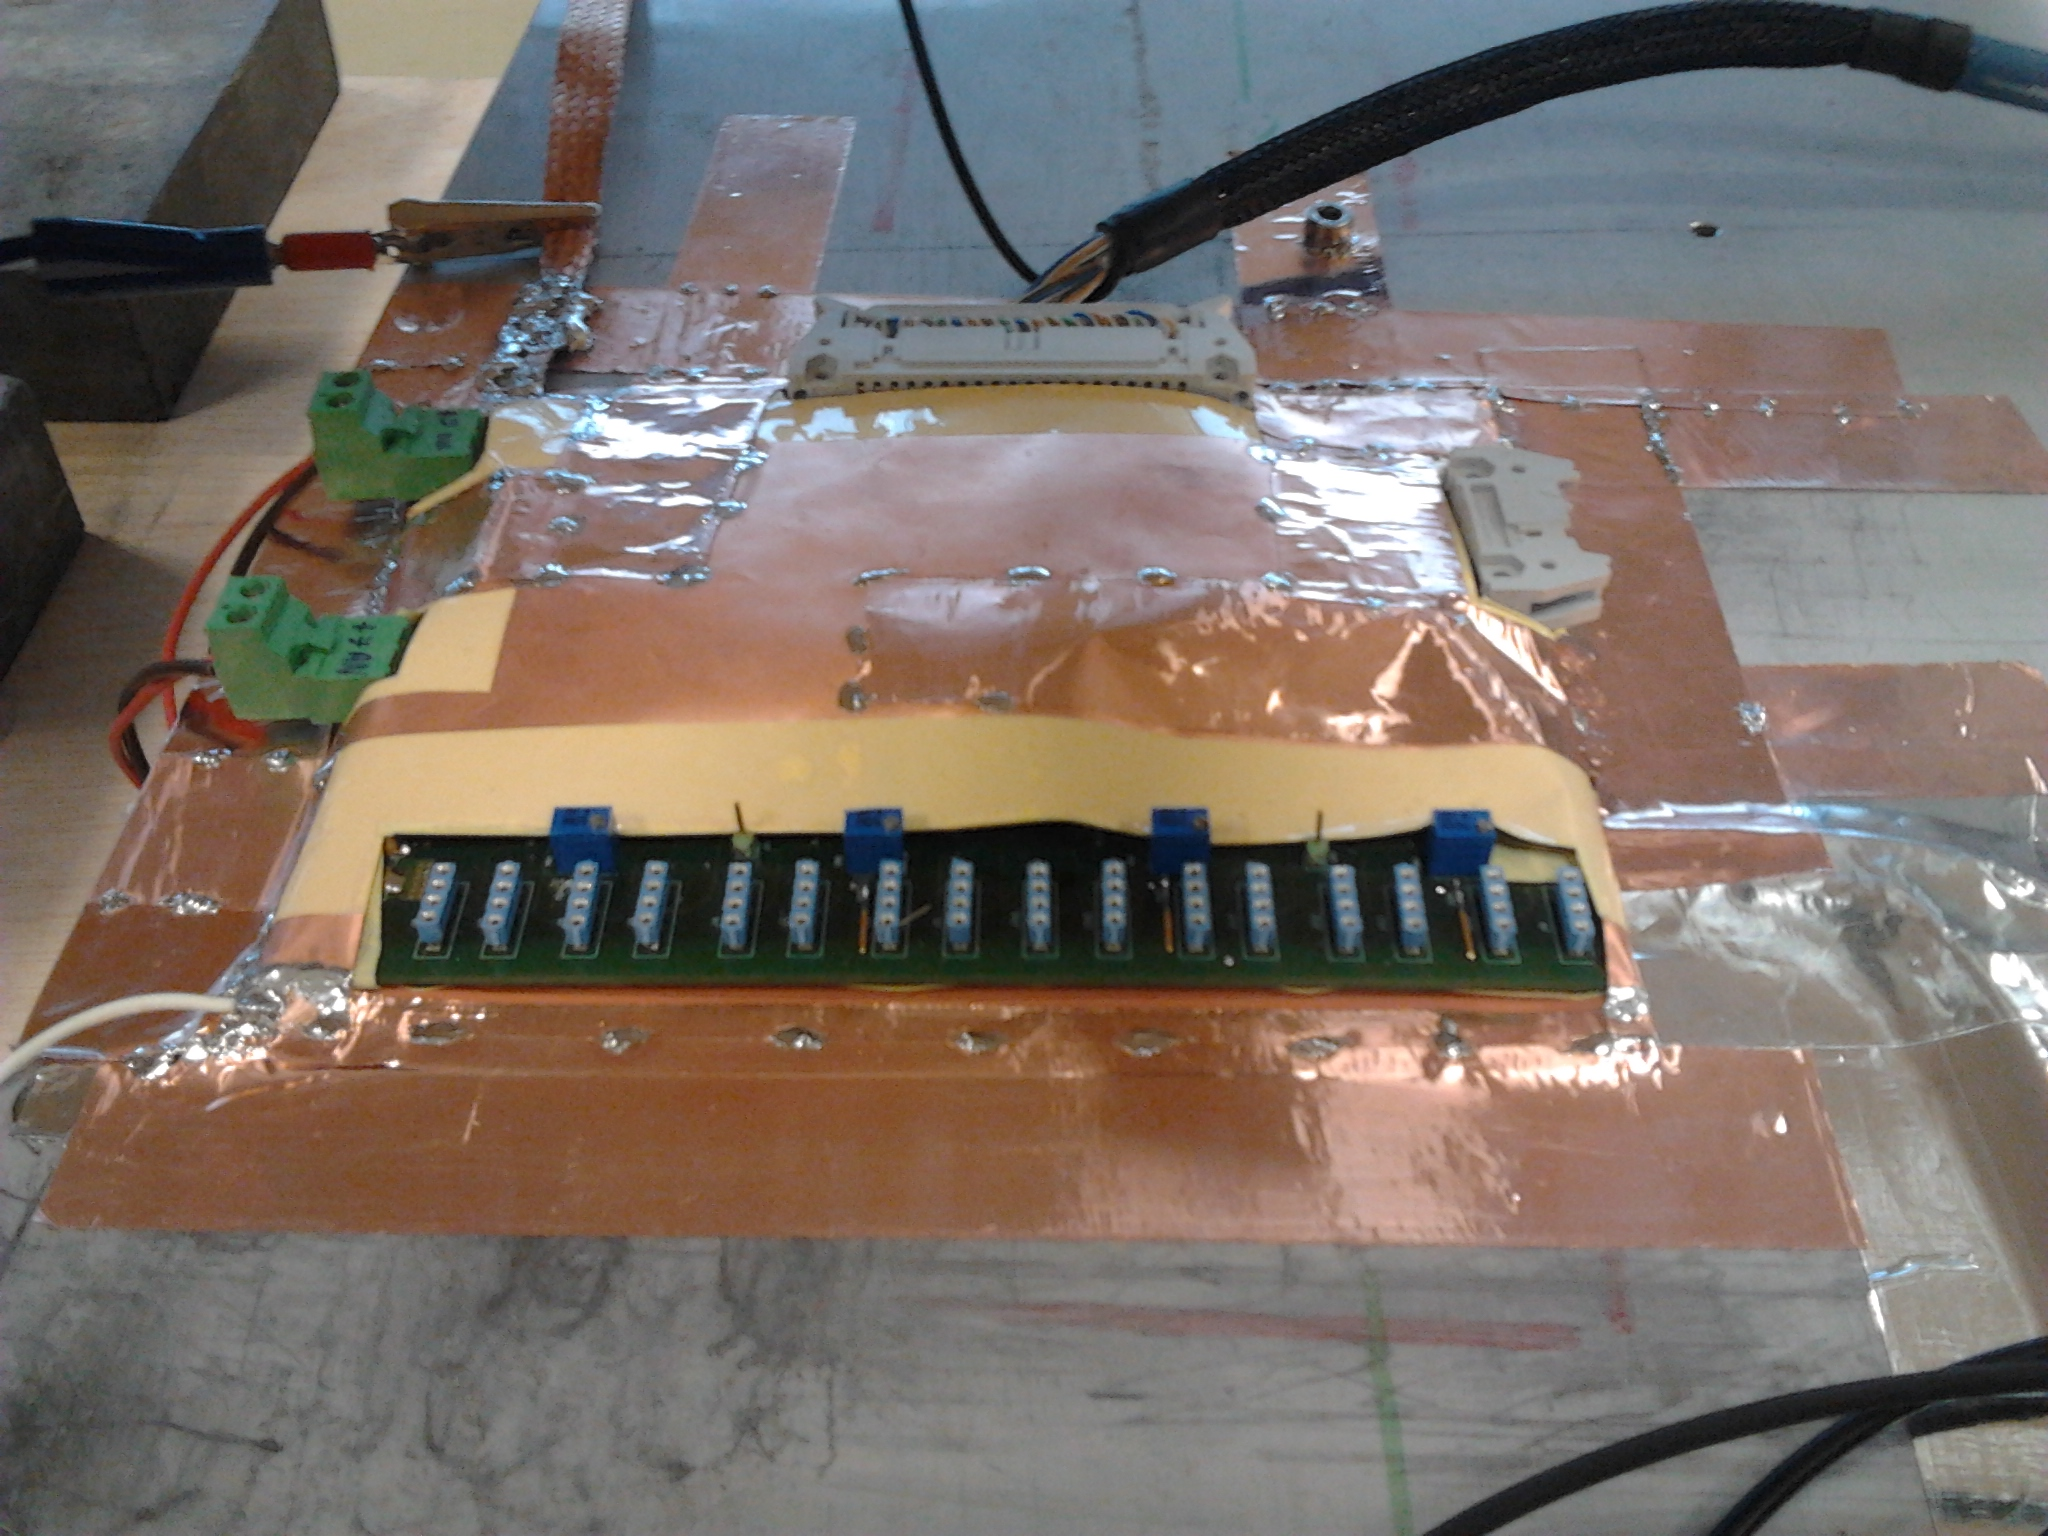
\includegraphics[height = 6cm]{fig/chapt6/ATLAS_FEB.png}
			\caption{\label{fig:Setup-INFN-904:A}}
		\end{subfigure}
		\begin{subfigure}{.4\linewidth}
		    \centering
			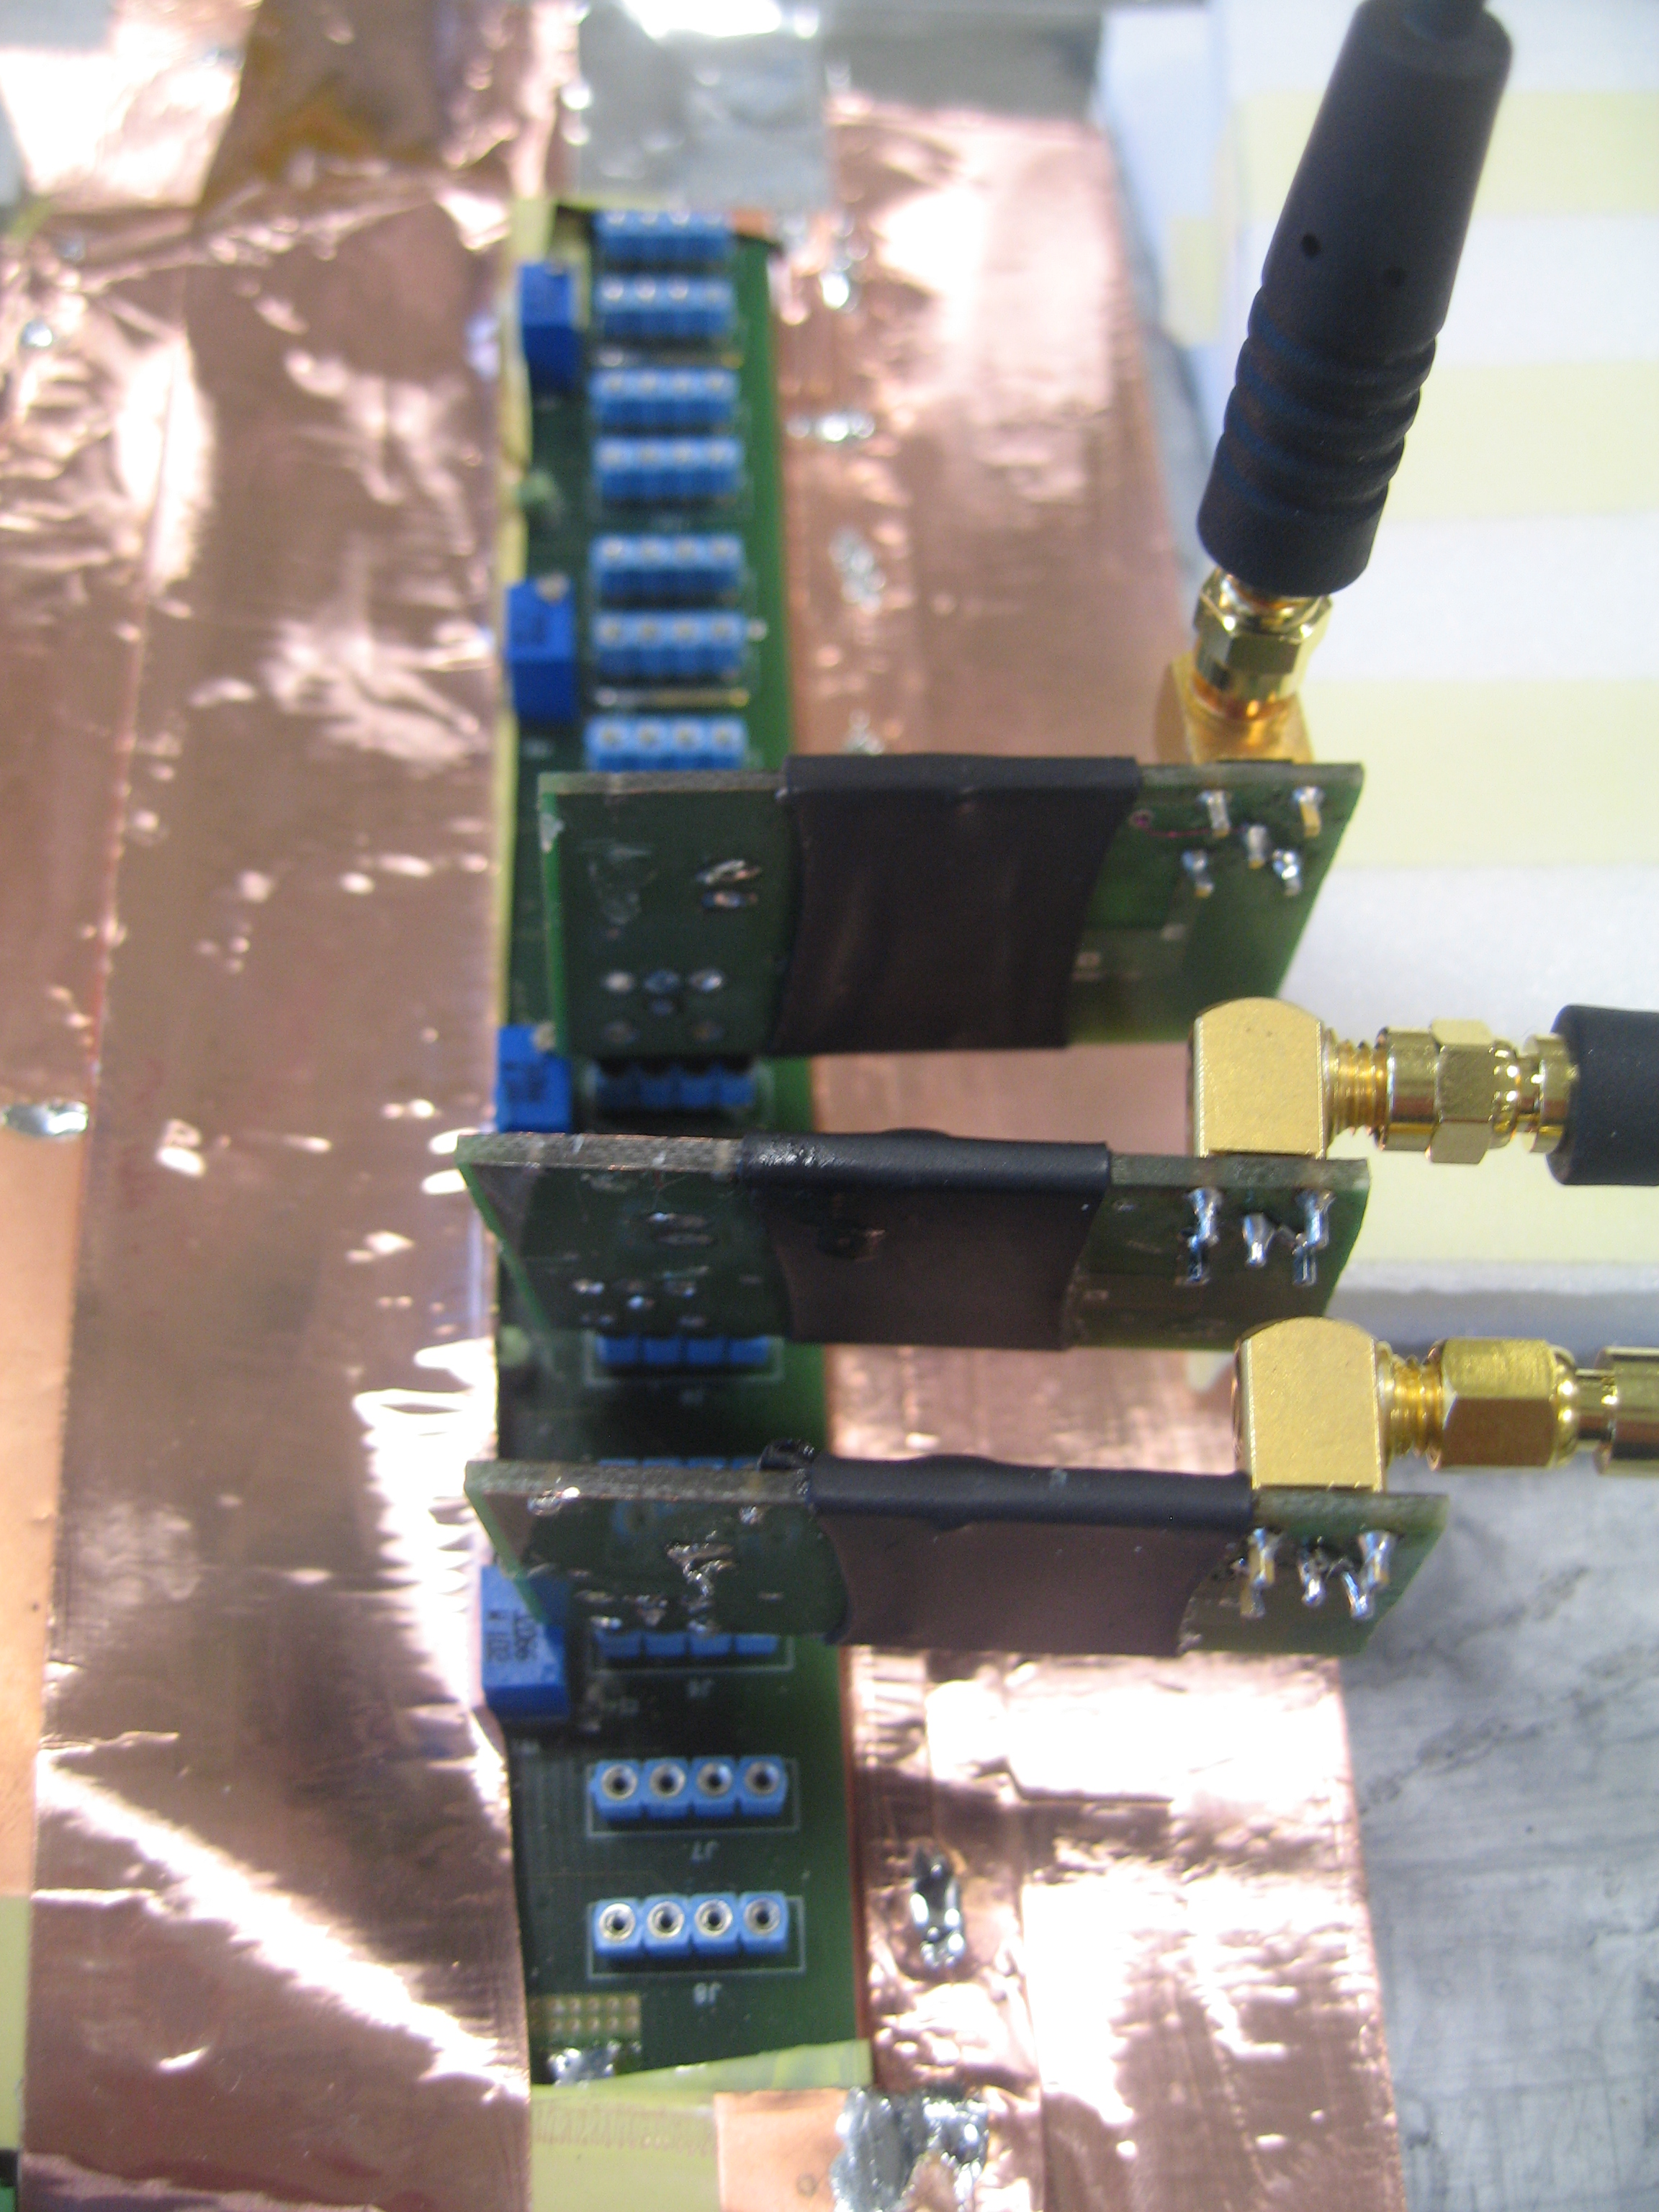
\includegraphics[height = 6cm]{fig/chapt6/ATLAS_preamp.JPG}
			\caption{\label{fig:Setup-INFN-904:B}}
		\end{subfigure}
		\begin{subfigure}{\linewidth}
		    \centering
			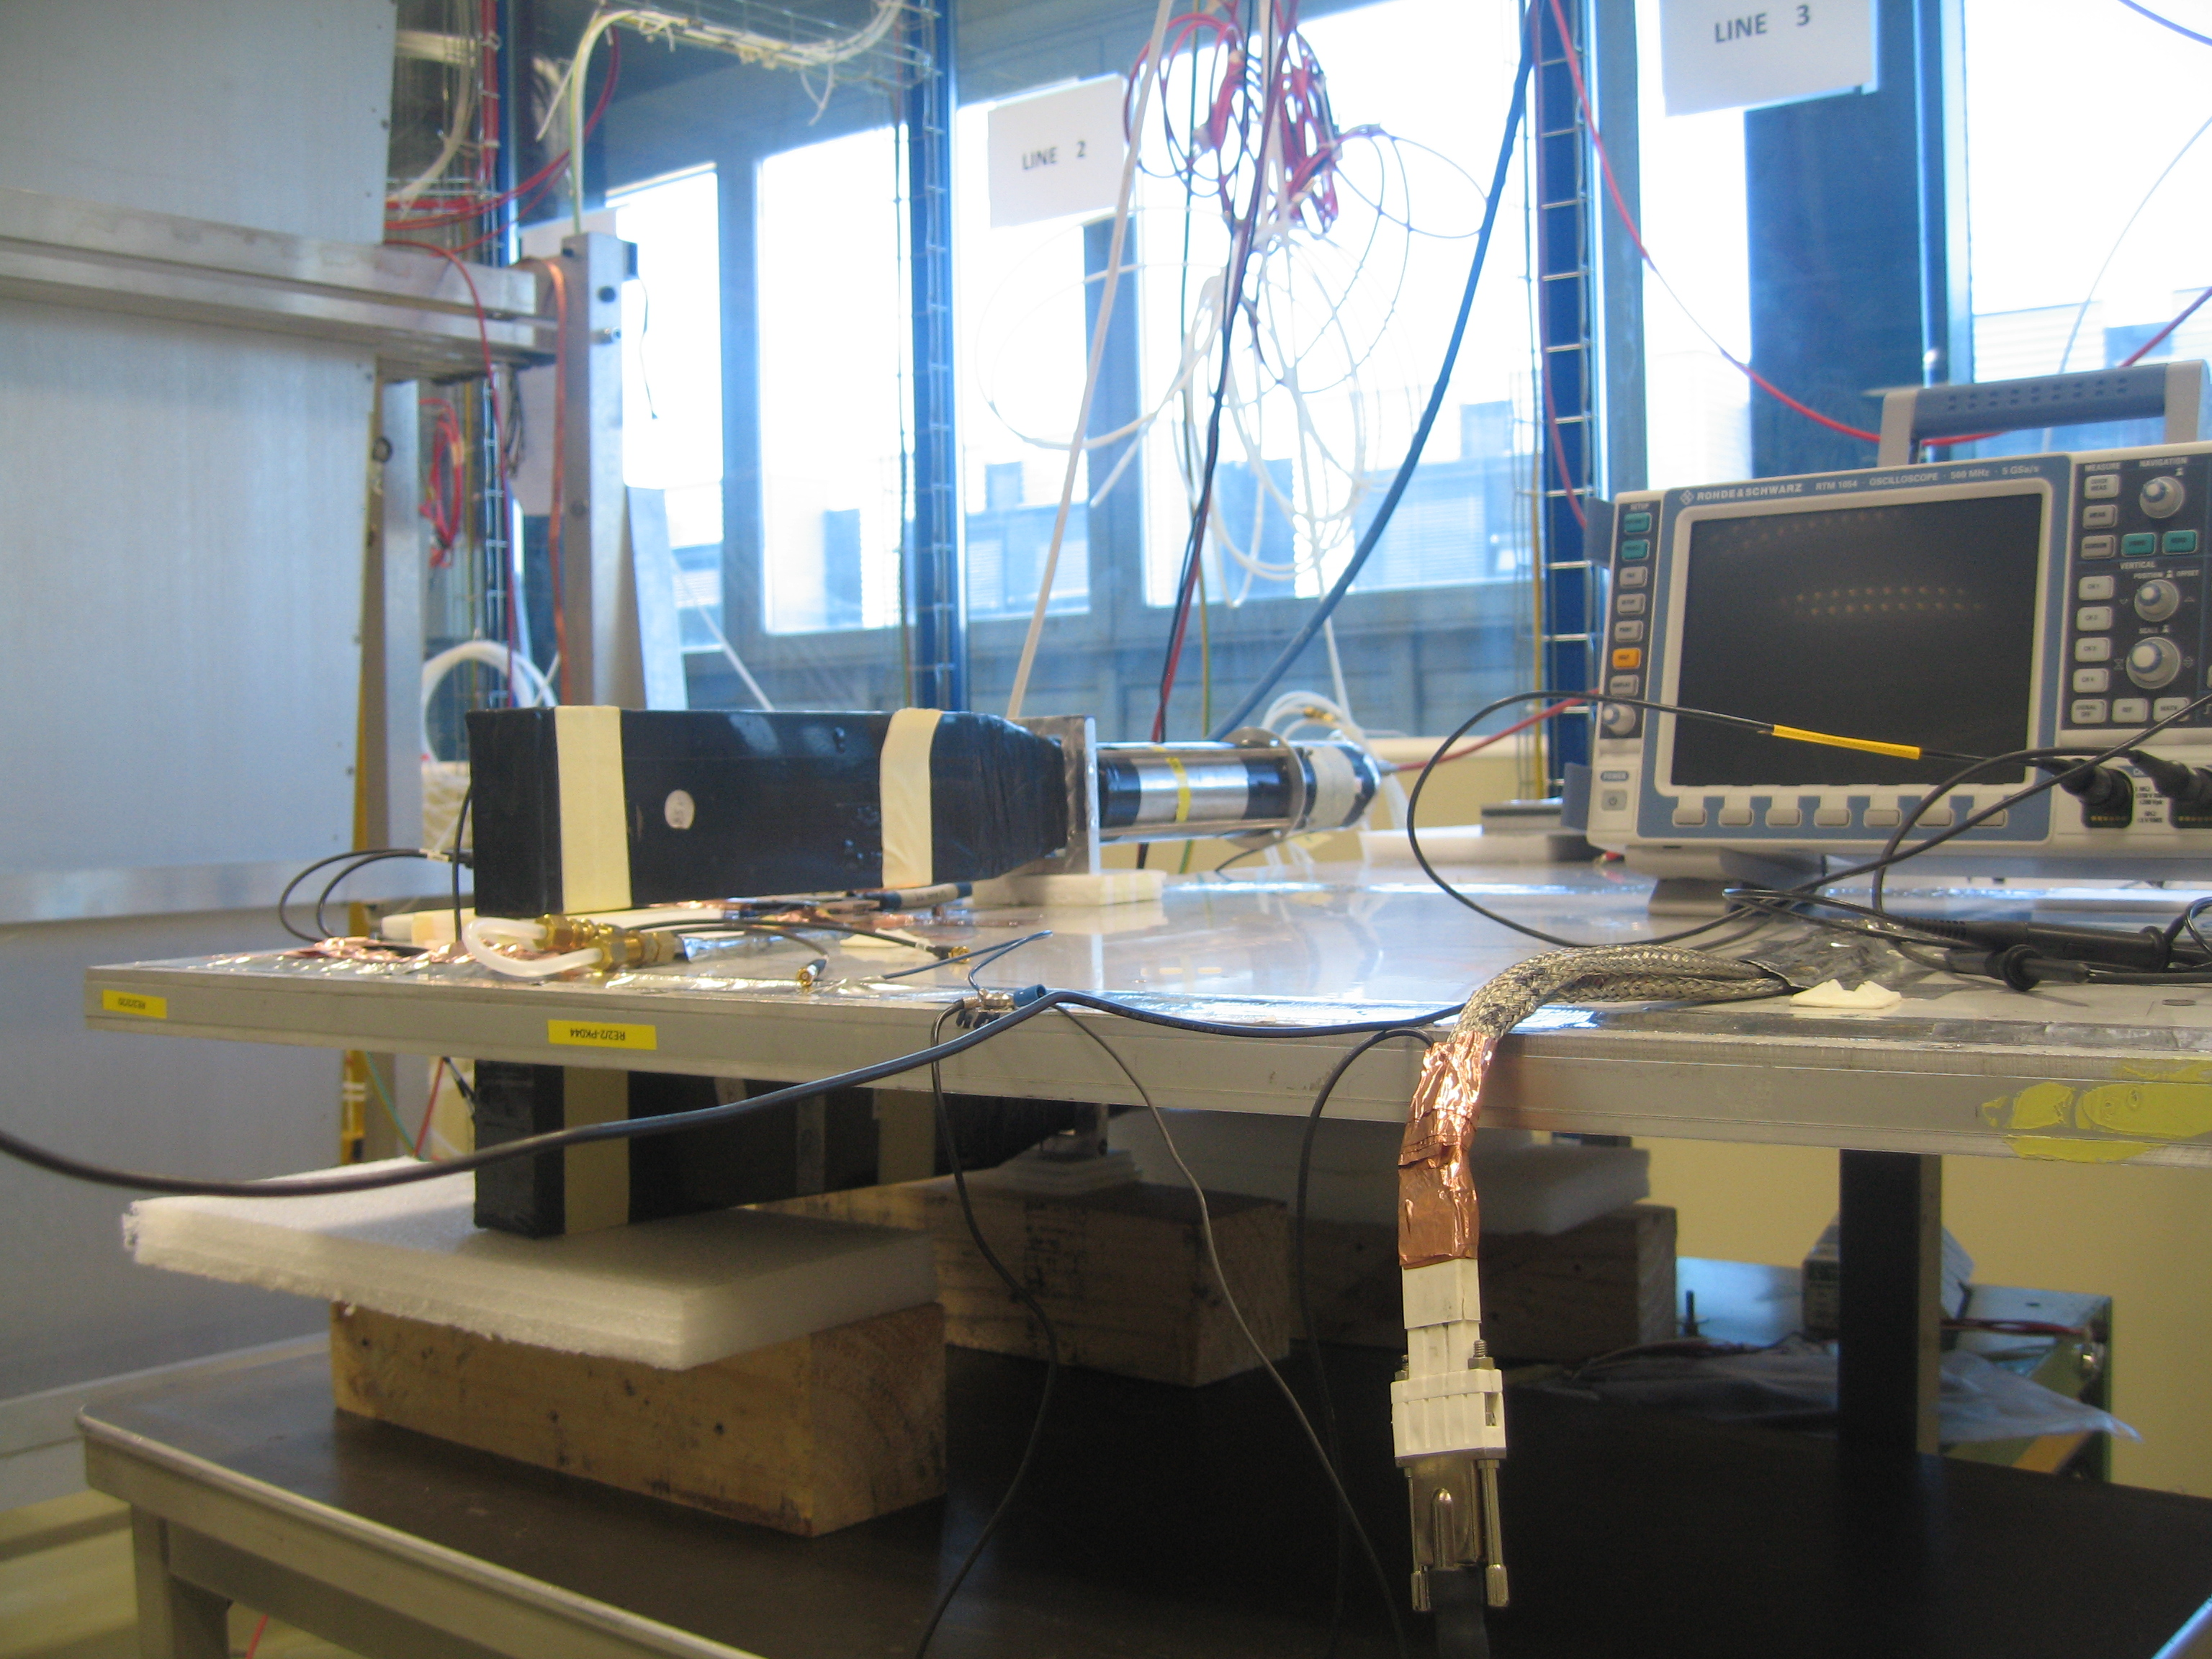
\includegraphics[height = 6cm]{fig/chapt6/Setup_ATLAS_PAK.JPG}
			\caption{\label{fig:Setup-INFN-904:C}}
		\end{subfigure}
		\caption{\label{fig:Setup-INFN-904} \subref{fig:Setup-INFN-904:A} Shielded \acl{FEB} on which the INFN preamplifiers are to be mounted. \subref{fig:Setup-INFN-904:B} Three INFN preamplifiers connected onto the test FEB. \subref{fig:Setup-INFN-904:C} Experimental setup used to test the INFN preamplifier single mounted on a FEB similar to the CMS FEB.}
    \end{figure}
	
	At the time of the second experiment, only three channels could be lent by the team of INFN Tor Vergata. The impedance of the preamplifiers was set to \SI{100}{\ohm} at delivery. The strips are then connected to the preamplifiers using \SI{50}{\ohm} coaxial cables equipped with SMC connectors, known for their good transmission. To match the impedance of the preamplifier input with the signal cable, a \SI{100}{\ohm} resistor was added in parallel of the input line. In CMS endcap RPCs, the strips are left floating. For the purpose of this test, it was necessary to terminate the strips on both ends to prevent reflections in the transmission line. The impedance of the strips being approximately \SI{25}{\ohm}, the strips were terminated with \SI{50}{\ohm} resistors on the signal cable side, and with \SI{25}{\ohm} resistors on the end side.\\
	The threshold of the zero-crossing discriminators used on the FEB is controlled via a LabVIEW interface similar to the one used to control the threshold of the CMS FEB. Various thresholds were used in a range in between 7 and \SI{5}{fC}. These values are a little higher than the minimal threshold of about \SI{3}{fC} used during the first experiment due to limitations of the FEB itself.\\
	Finally, it was decided to use the same PMTs than in the first experiment as trigger. This time, they were placed on their narrow side to only cover an area on the detector smaller than three strips. On the data acquisition side, no DAQ software was available yet at the time of experimentation and scalers were once again used. As can be seen from Figure~\ref{fig:Pulse-Processing-904}, the pulse processing has been inspired by the previous scheme. Thanks to the lower number of channels to monitor, the cluster size could be estimated by counting the signals on single channels (A, B and C on their own) but also on groups of two (A and B, B and C) and three channels (A and B and C) in coincidence with the trigger.
	
	\begin{figure}[H]
		\centering
		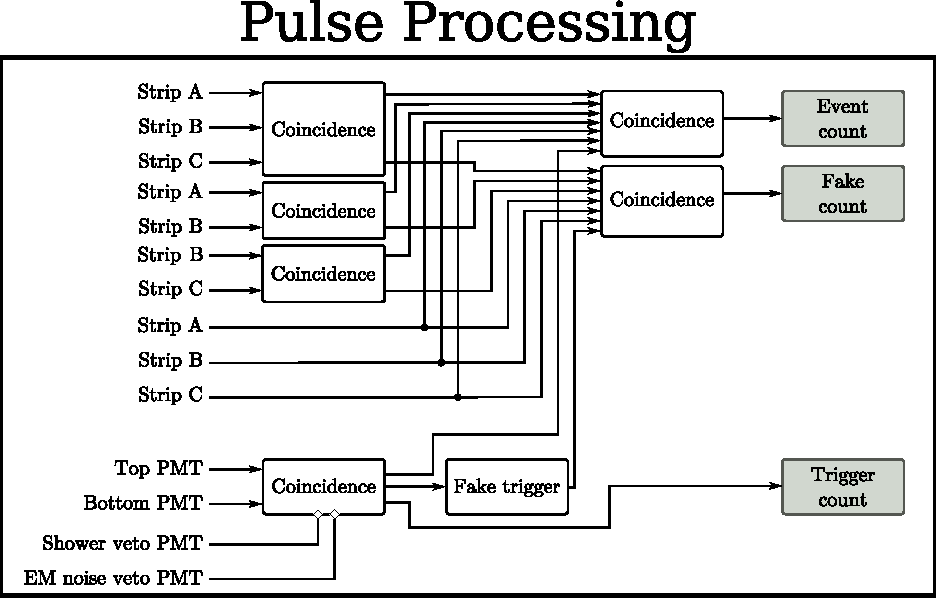
\includegraphics[width=.9\linewidth]{fig/chapt6/pulse-processing-2014.pdf}
		\caption{\label{fig:Pulse-Processing-904} Similarly to Figure~\ref{fig:Pulse-Processing:C}, the signals are counted in coincidence with the trigger signals provided by PMTs. To estimate the cluster size, the channels are counted by groups of three, two but also alone.}
	\end{figure}
	
	The results of the second round of tests with INFN preamplifiers are presented in Figure~\ref{fig:INFN-FEB} and Table~\ref{tab:INFN-FEB}. These results are consistent with what was measured with the first tested prototypes. The efficiency sigmoid has been measured once again with the CMS FEB, using a threshold of \SI{146}{fC} and is in agreement with the data collected in 2013. The performance of the detector with the preamplifiers tuned at 7.2 and \SI{6.4}{fC} falls in the very same values than the setting at \SI{7}{fC} according to the table. A maximum shift of \SI{410}{V} is observed for a threshold of \SI{5}{fC}.\\
	With the care placed into having a good grounding of the setup as well as a good impedance matching, the noise rate per unit area is this time lower than what previously measured. Nevertheless, it still is more than one order of magnitude higher than in the case of the CMS FEB with a threshold set at \SI{146}{fC}. The noise rate is measured to be at lowest around \SIrate{0.7} when measured to be approximately \SIrate{0.05} for the CMS FEB. At such high threshold values, the noise rate per unit area is not expected to vary much. The data collected at the RPC assembly laboratory then displays much better data tacking conditions with both electronics.\\
	Finally, the cluster size is measured to be similar for both electronics at the level of the working point and is in between 2.2 and 2.4 strips on average. The spatial resolution of both devices would then be the same.
	
	\begin{figure}[H]
		\begin{subfigure}{.5\linewidth}
		    \centering
			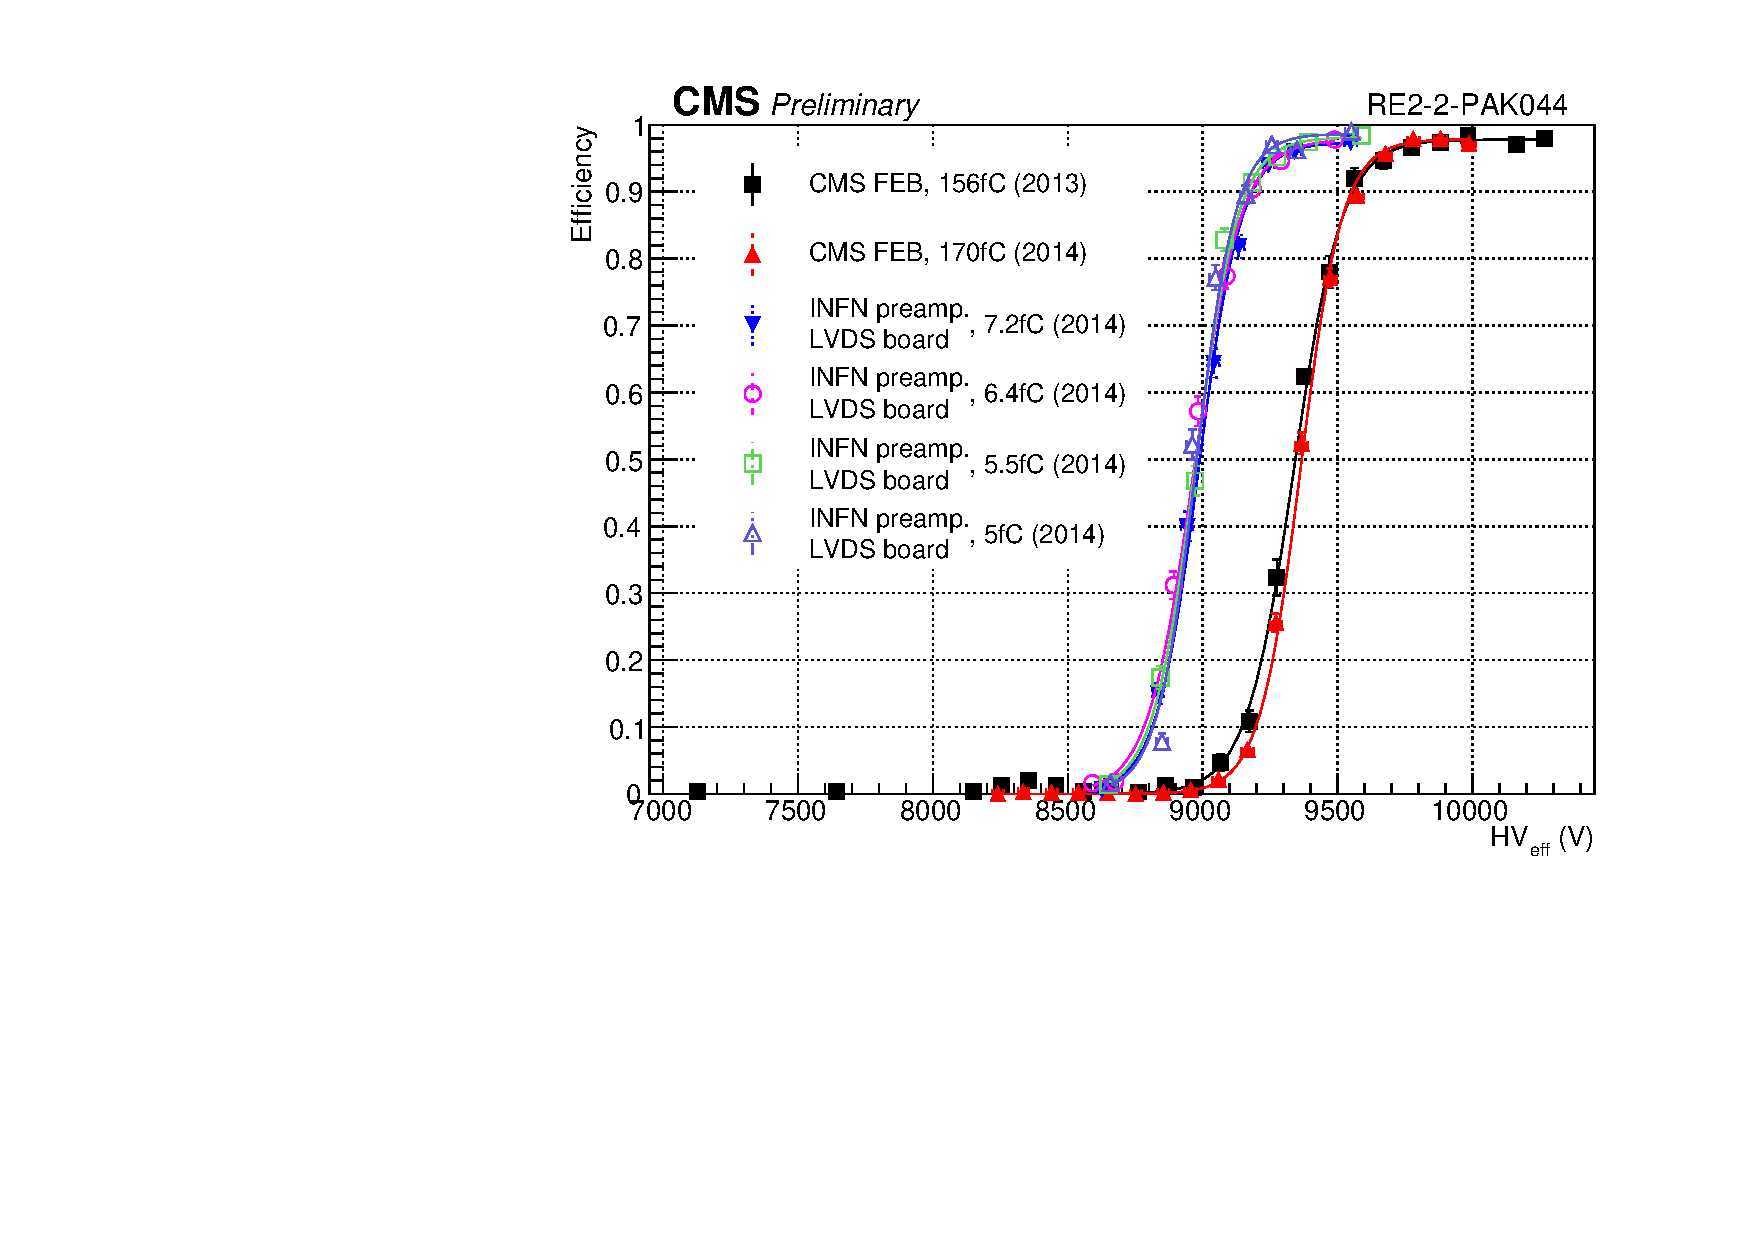
\includegraphics[width=\linewidth]{fig/chapt6/INFN-LVDS-Eff-Shift.pdf}
			\caption{\label{fig:INFN-FEB:A}}
		\end{subfigure}
		\begin{subfigure}{.5\linewidth}
		    \centering
			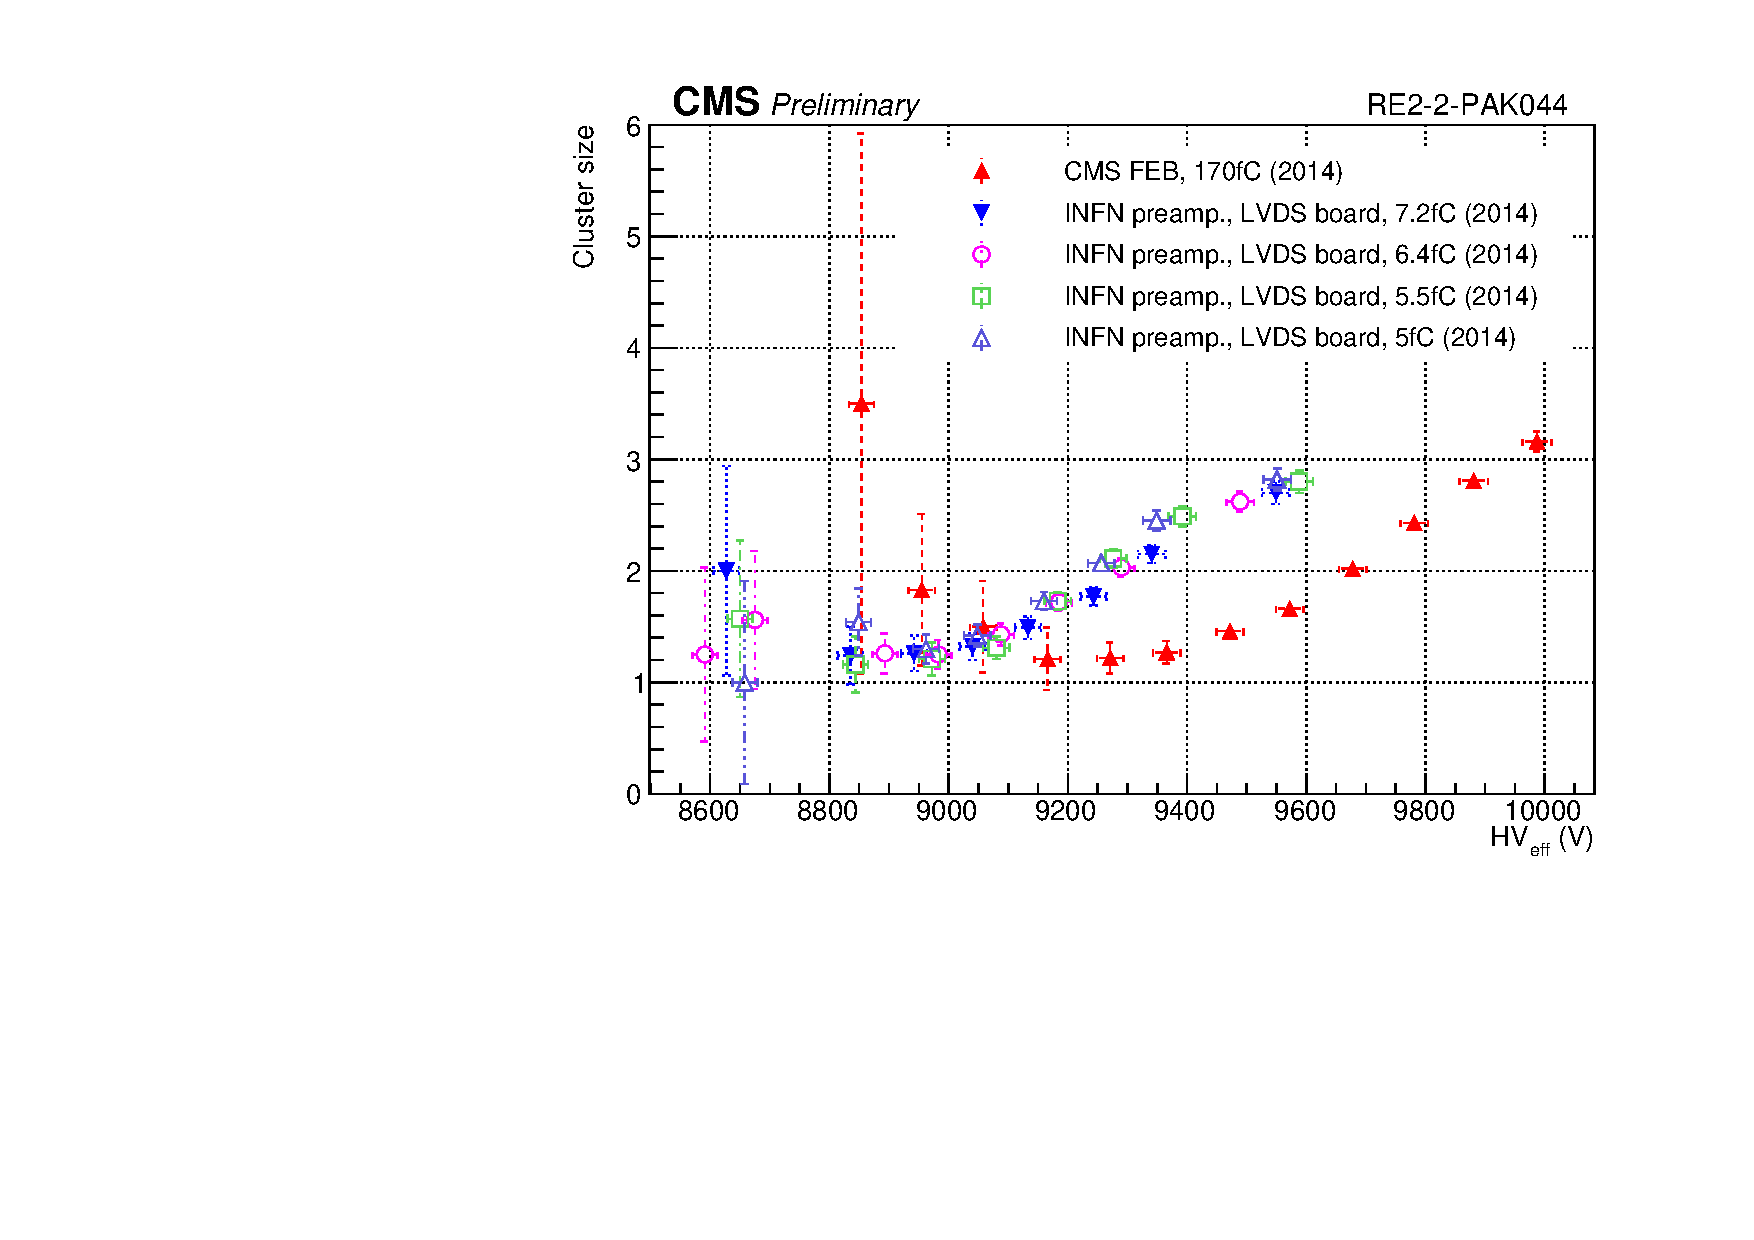
\includegraphics[width = \linewidth]{fig/chapt6/INFN-LVDS-ClS-Shift.pdf}
			\caption{\label{fig:INFN-FEB:B}}
		\end{subfigure}
		\begin{subfigure}{\linewidth}
		    \centering
			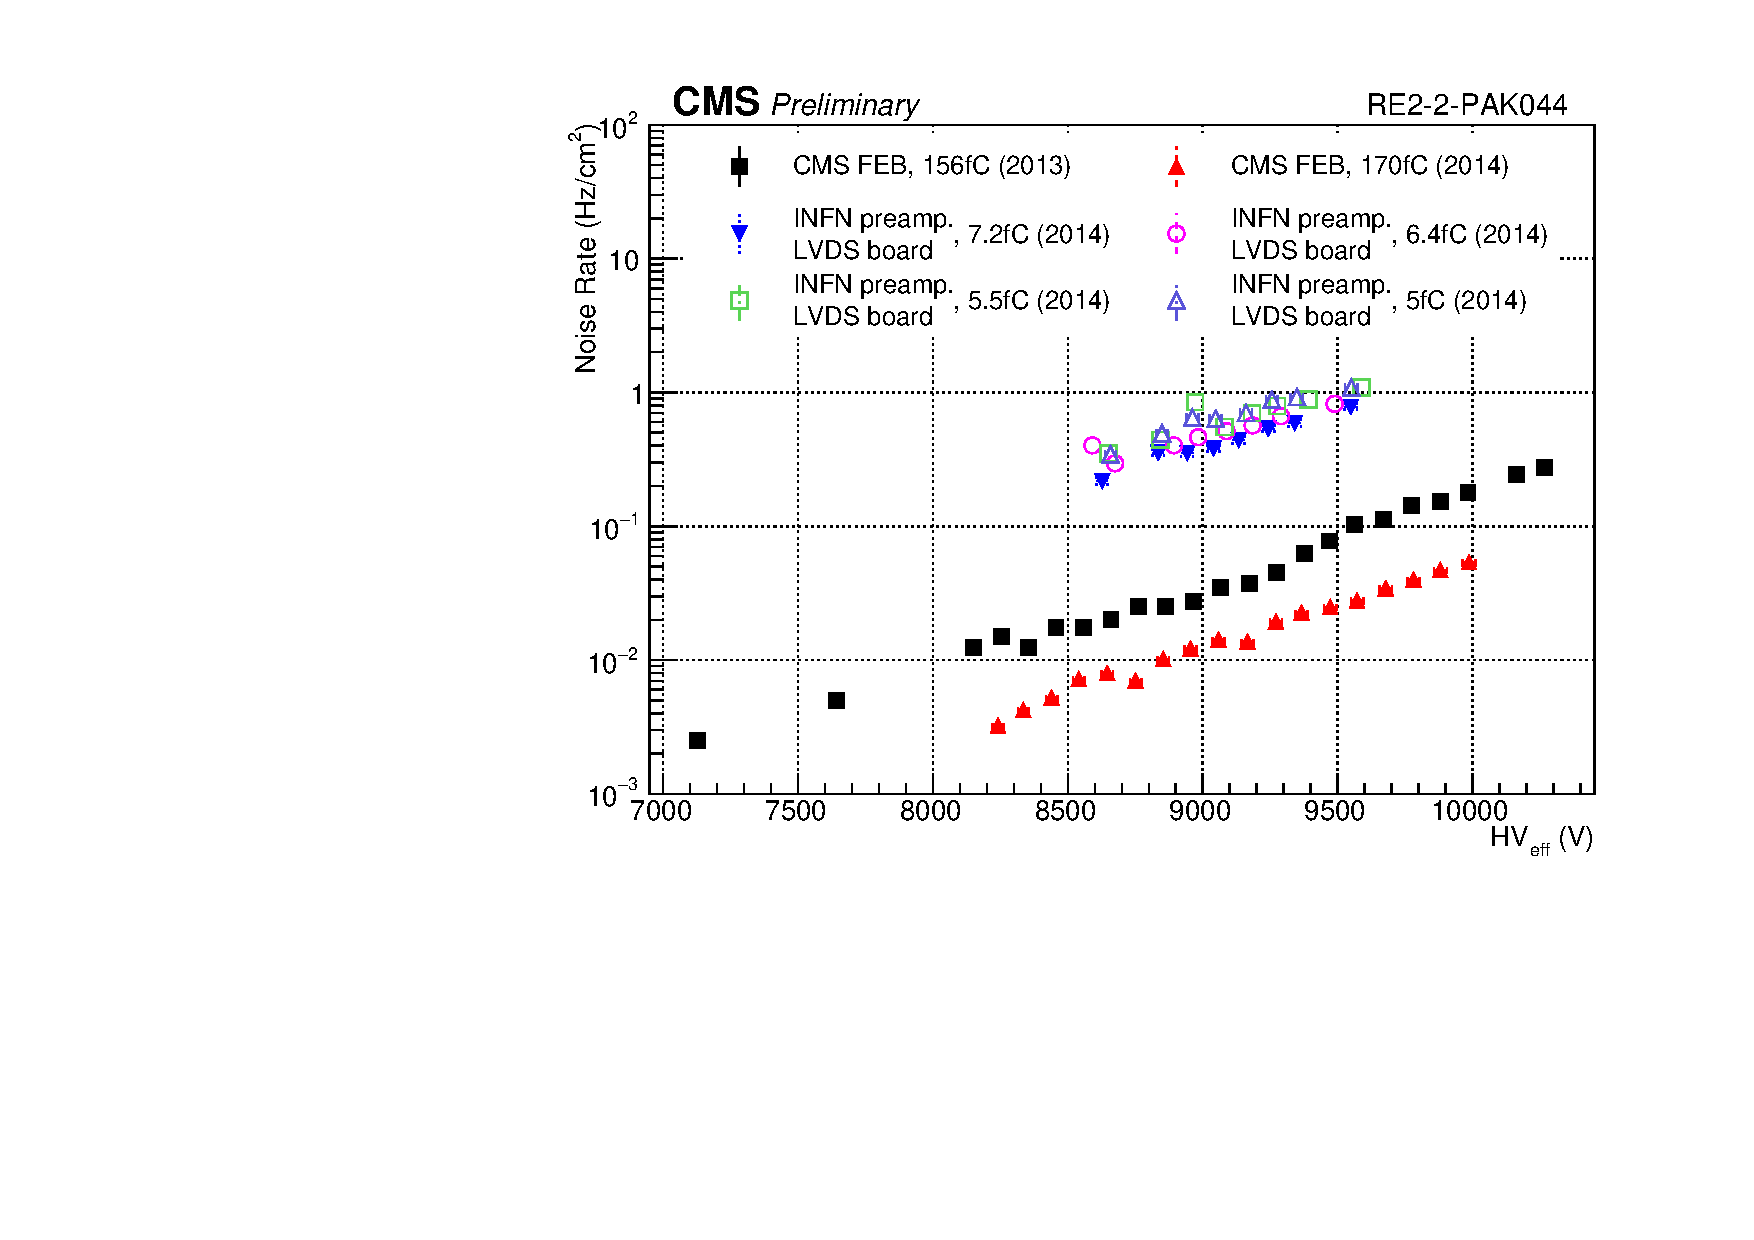
\includegraphics[width = .5\linewidth]{fig/chapt6/INFN-LVDS-Rate-Shift.pdf}
			\caption{\label{fig:INFN-FEB:C}}
		\end{subfigure}
		\caption{\label{fig:INFN-FEB} Efficiency~\subref{fig:INFN-FEB:A}, cluster size~\subref{fig:INFN-FEB:B} and noise rate per unit area~\ref{fig:INFN-FEB:C} of the CMS RE2-2 detector tested with the standard CMS FEBs (black and red) and with the INFN preamplifier mounted onto the CMS FEB at different thresholds (blue, pink, green and purple).}
	\end{figure}
	
	\begin{table}[H]
		\caption{\label{tab:INFN-FEB} Results of the sigmoid fit (Equation~\ref{eq:Sigmoid}) performed on the data presented in Figure~\ref{fig:INFN-FEB:A}. The working point and its corresponding efficiency are computed using Equations~\ref{eq:Sigmoid} and \ref{eq:KneeWP}.}
		\footnotesize
		\begin{tabular}{|c|c|c|c|c|c|}
			\hline
Data & $\epsilon_{max}$ & $\lambda$ ($\cdot$\Ord{-2} \si{V^{-1}}) & $HV_{50}$ (\si{V}) & $\epsilon_{WP}$ & $HV_{WP}$ (\si{V}) \\ 
			\hline
CMS FEB, 143fC (2013)      & $0.978 \pm 0.004$ & $1.12 \pm 0.07$ & $9339 \pm 11$ & $0.97 \pm 0.01$ & $9752 \pm 27$\\ 
			\hline
CMS FEB, 146fC (2014)      & $0.978 \pm 0.003$ & $1.30 \pm 0.06$ & $9364 \pm 9$  & $0.97 \pm 0.01$ & $9740 \pm 19$\\ 
			\hline
INFN/CMS FEB, 7.2fC (2014) & $0.973 \pm 0.006$ & $1.26 \pm 0.09$ & $8985 \pm 10$ & $0.97 \pm 0.01$ & $9368 \pm 26$\\ 
			\hline
INFN/CMS FEB, 6.4fC (2014) & $0.978 \pm 0.007$ & $1.16 \pm 0.08$ & $8969 \pm 11$ & $0.97 \pm 0.01$ & $9372 \pm 28$\\ 
			\hline
INFN/CMS FEB, 5.5fC (2014) & $0.981 \pm 0.005$ & $1.26 \pm 0.09$ & $8973 \pm 12$ & $0.97 \pm 0.01$ & $9357 \pm 28$\\ 
			\hline
INFN/CMS FEB, 5fC (2014)   & $0.987 \pm 0.004$ & $1.37 \pm 0.10$ & $8976 \pm 12$ & $0.98 \pm 0.01$ & $9342 \pm 28$\\ 
			\hline
		\end{tabular}
	\end{table}
	
	In addition to the tests performed on the electronics with the CMS RPC, the electronics also have been tested on a gRPC designed in Ghent. The gRPC used for this experiment is described in Figure~\ref{fig:UGent-gRPC-design}. The detector, shown on Figure~\ref{fig:UGent-gRPC-pictures}, uses a double-gap layout with float glass electrodes of \SI{1.1}{mm} and a gas gap of \SI{1.2}{mm}. The electrodes themselves are made out of four pieces of glass glued together. Such a design was studied for high-rate detection purposes and aimed to serve as a proof of concept for RPCs built using small pieces assembled together to produce a larger detection area. Indeed, in the context of R\&D in the field of high-rate RPCs, most low resistivity materials are custom made dopped glass or ceramics plates. These materials can't be produced in large areas as they are not manufactured on a large enough scale. Thus, building large detectors can imply using such methods.
    
    The tests involving this detector were conducted in 2015 with the setup described by Figure~\ref{fig:Setup-INFN-gRPC}. The photomultipliers used to trigger the data taking were a little larger than the detector and the strips themselves. Similarly to the case of the GIF experiment described in Section~\ref{chapt5:ssec:GeoAcc} of Chapter~\ref{chapt5}, it has been necessary to evaluate the geometrical acceptance of the setup to detect cosmic muons. This way, a C++ Monte Carlo simulation has been written using the dimensions of the experimental setup. By running 1000 simulations in which a million muons were generated in a source plane much larger than the experimental setup itself to reach high zenith angles, the geometrical acceptance was measured to be \numerror{0.9835}{0.0014}. This factor has then been used to correct the measured efficiency of the detector.
	 
	\begin{figure}[H]
		\begin{subfigure}{\linewidth}
		    \centering
			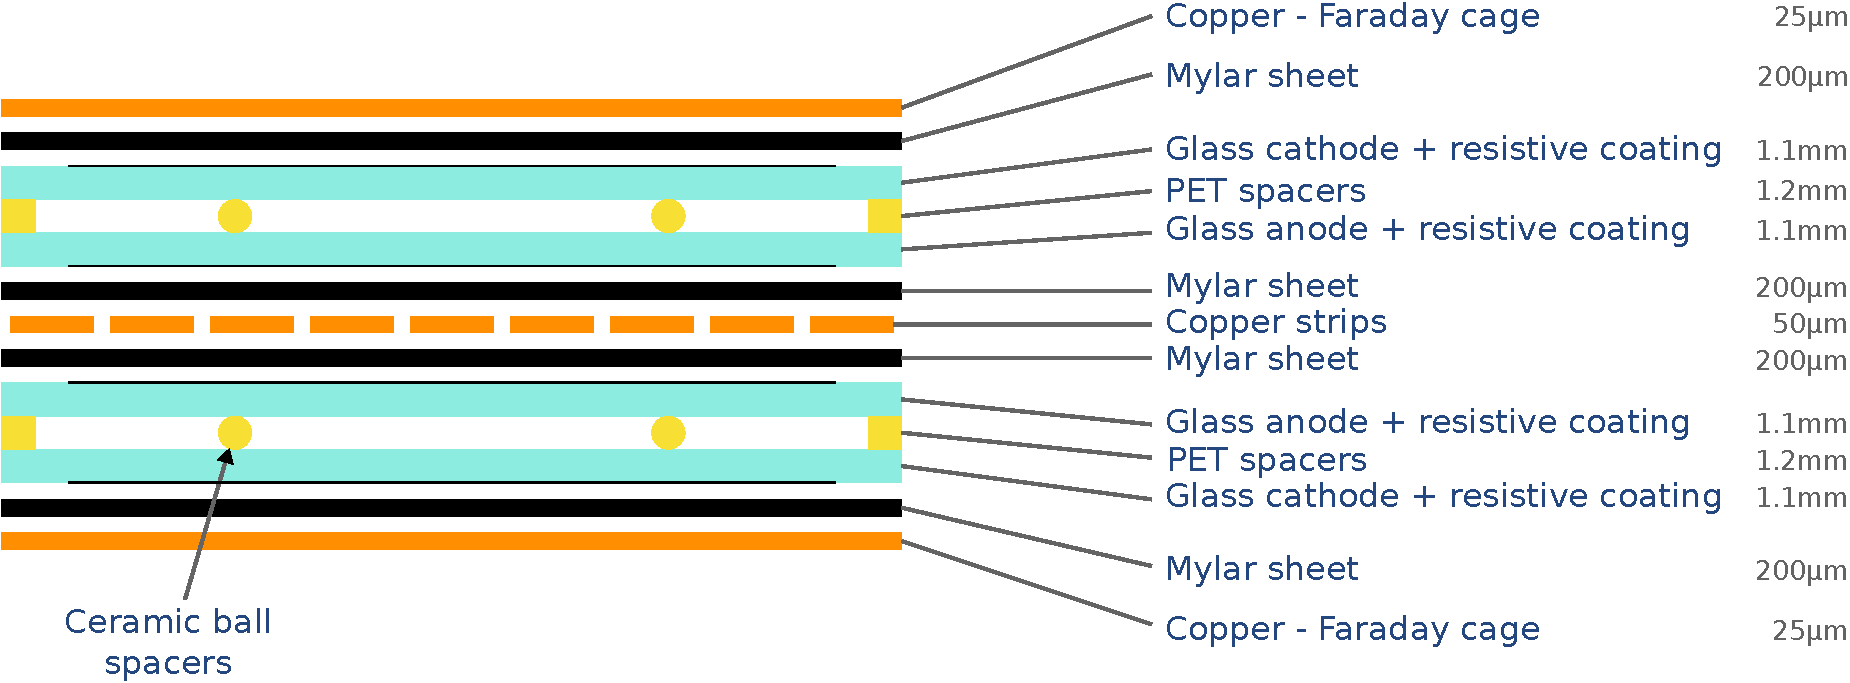
\includegraphics[width = .8\linewidth]{fig/chapt6/gRPC-design.pdf}
			\caption{\label{fig:UGent-gRPC-design:A}}
		\end{subfigure}
		\begin{subfigure}{\linewidth}
		    \centering
			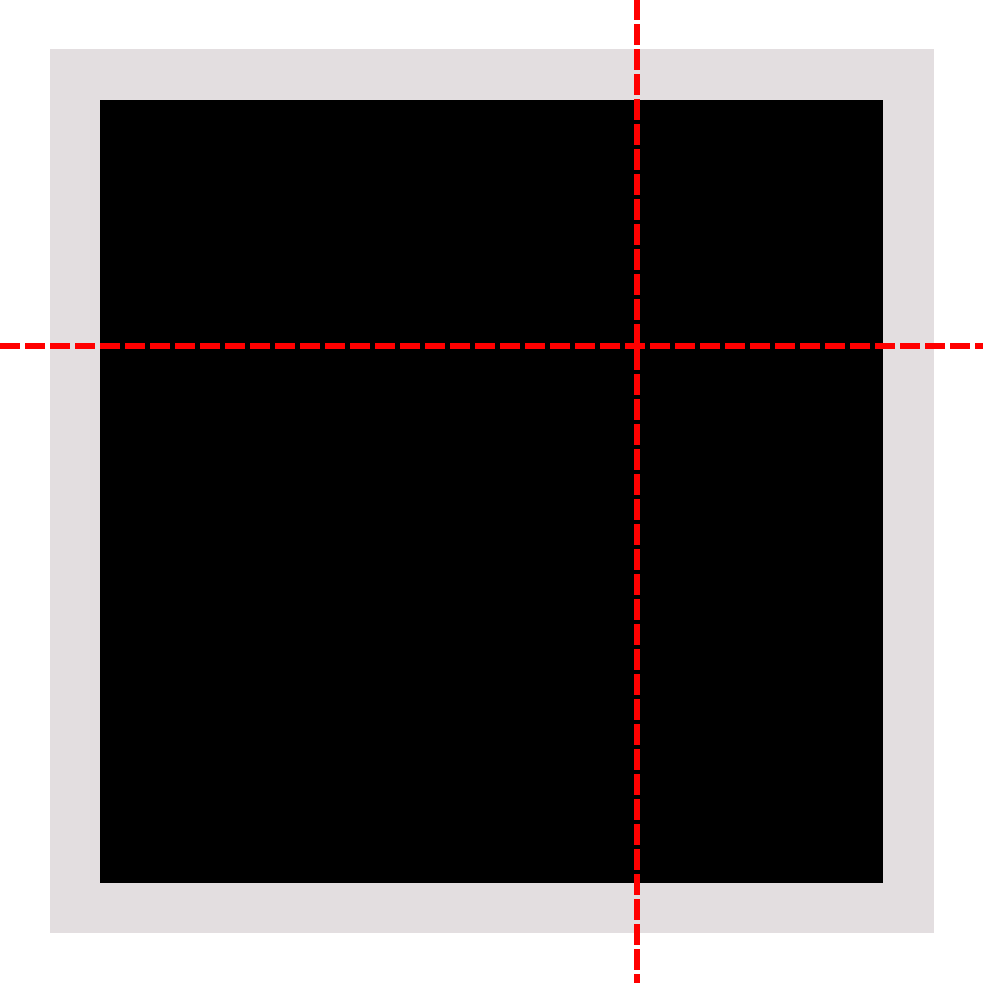
\includegraphics[width = .35\linewidth]{fig/chapt6/gRPC-assembly.pdf}
			\caption{\label{fig:UGent-gRPC-design:B}}
		\end{subfigure}
		\caption{\label{fig:UGent-gRPC-design} \subref{fig:UGent-gRPC-design:A}) The glass RPC developped by Ghent uses a double-gap design. \subref{fig:UGent-gRPC-design:B} The electrodes are made of four pieces of float glass glued into a single plate. Indeed a gluing technique has been investigated as most new low resistivity materials foreseen for RPCs of the new generation are not available in large areas.}
    \end{figure}
	 
	\begin{figure}[H]
		\begin{subfigure}{.5\linewidth}
		    \centering
			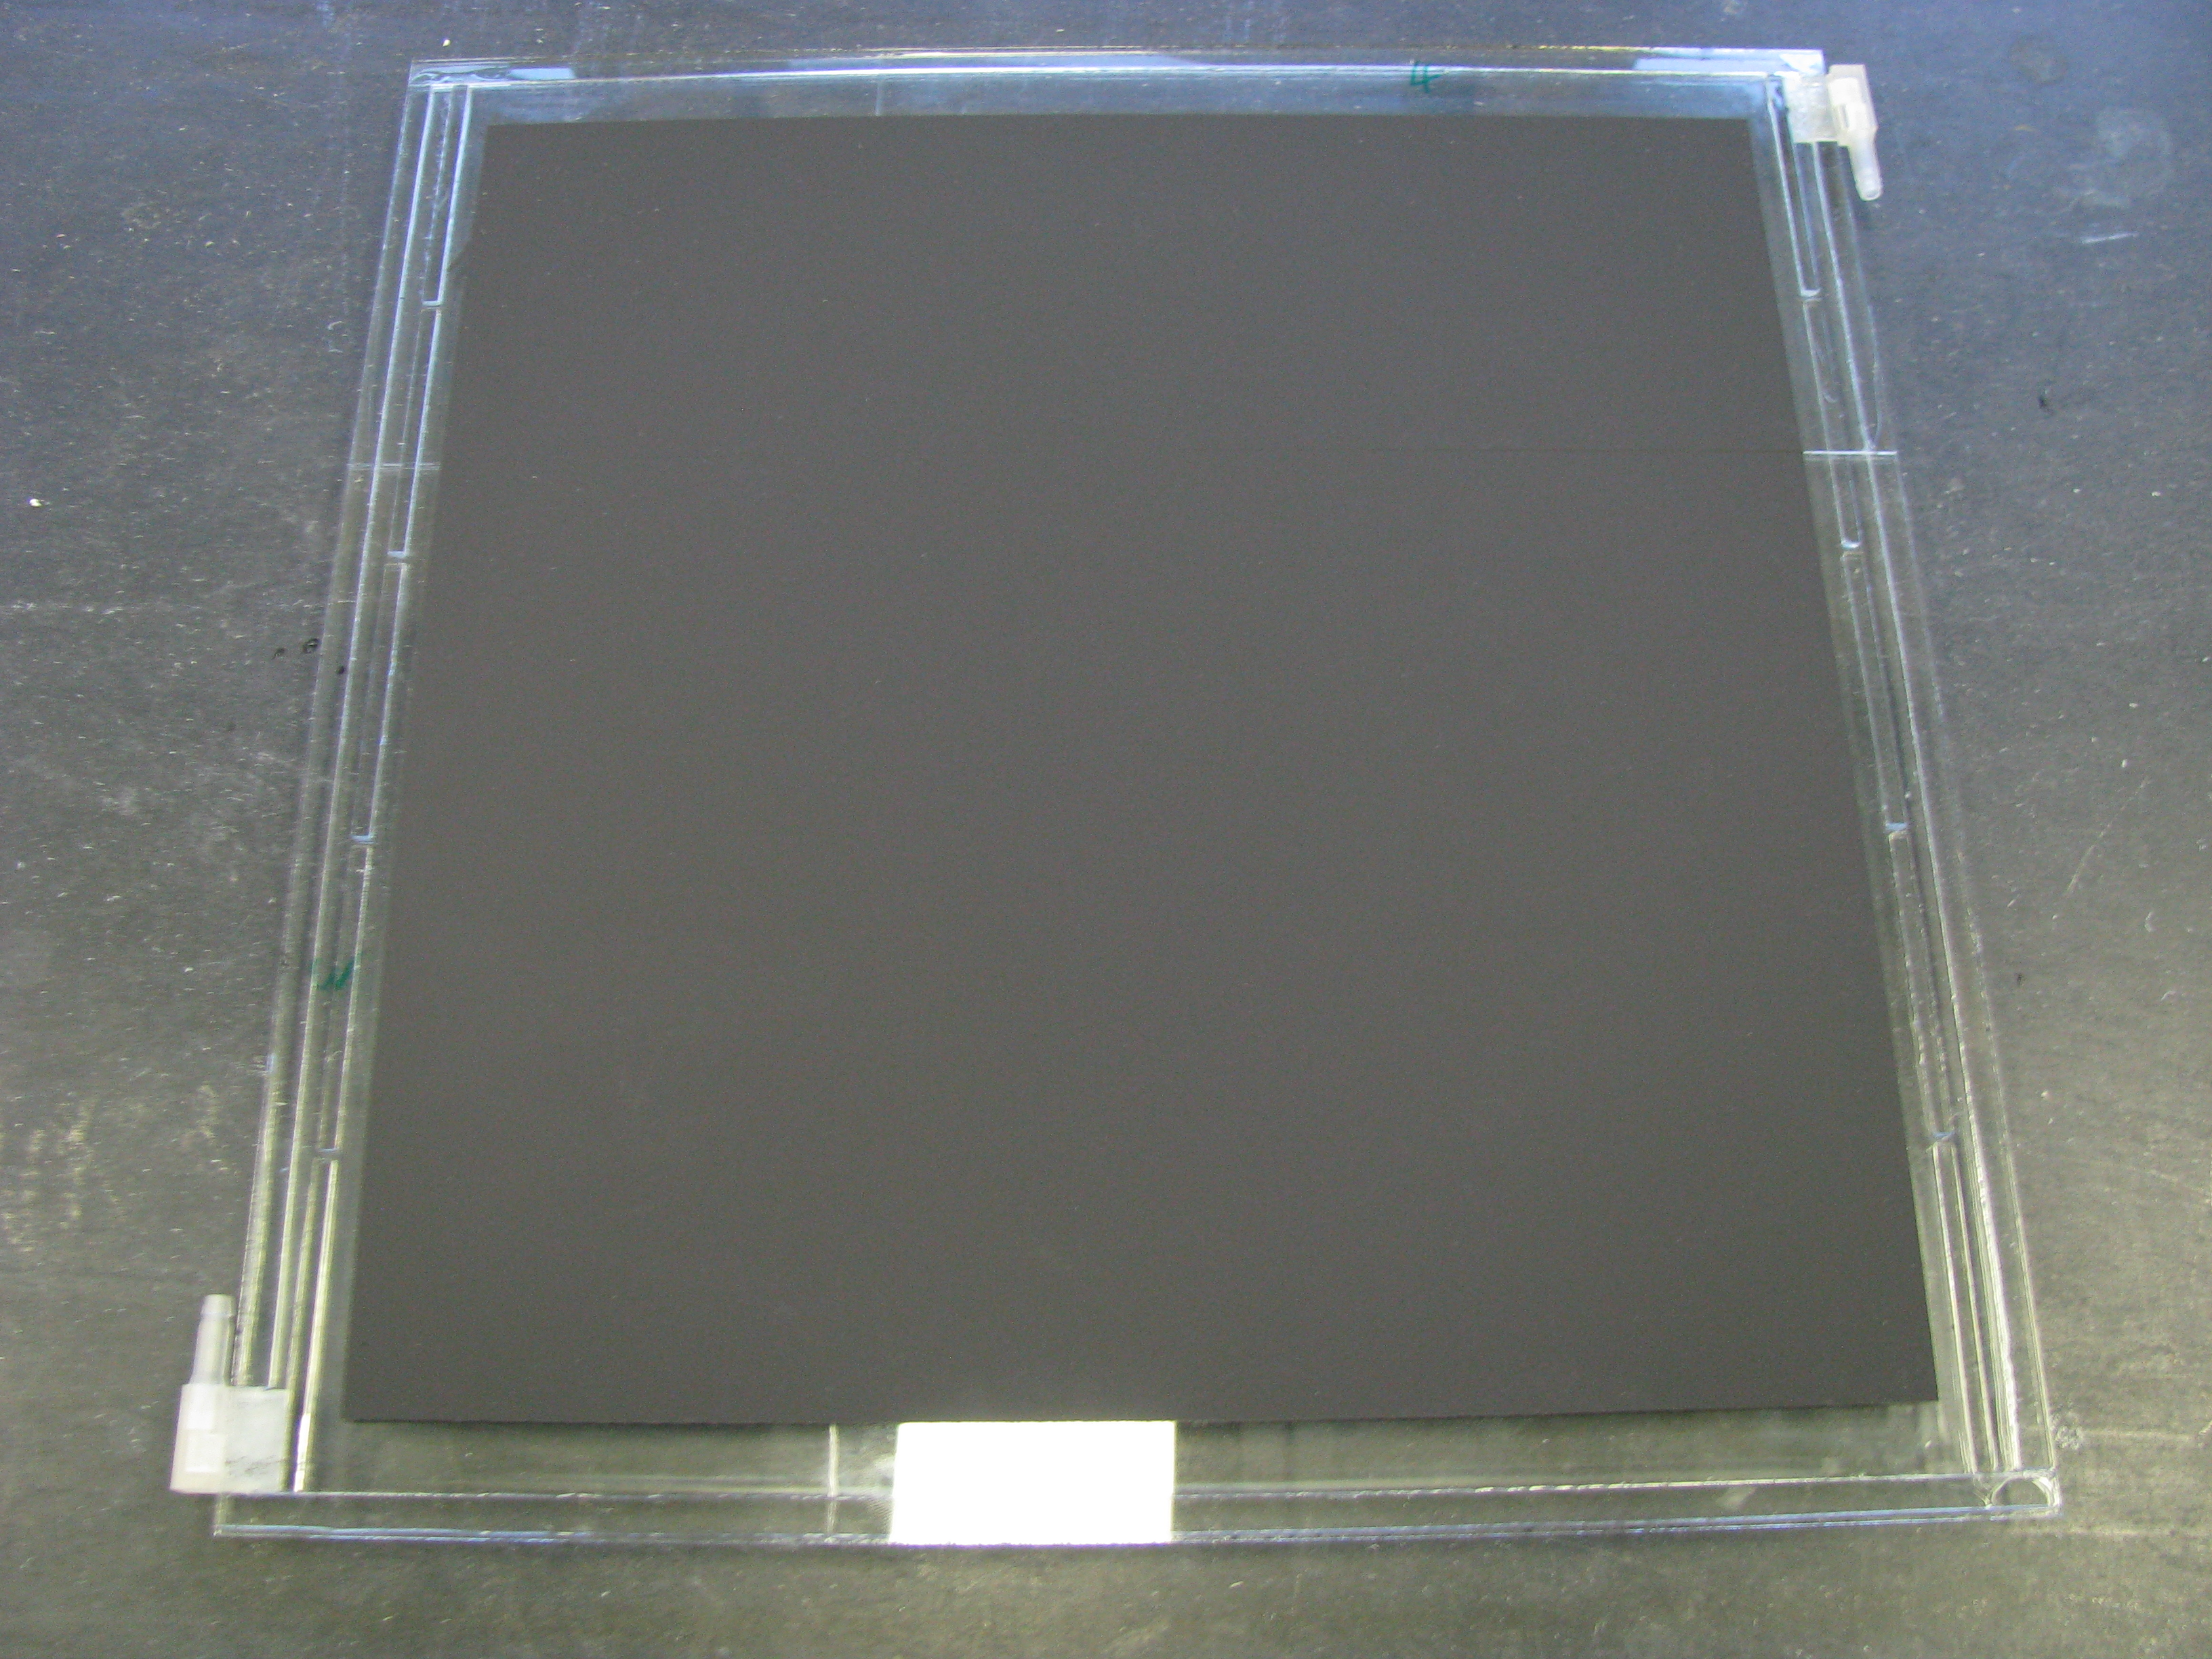
\includegraphics[width = .9\linewidth]{fig/chapt6/gRPC-gap.JPG}
			\caption{\label{fig:UGent-gRPC-pictures:A}}
		\end{subfigure}
		\begin{subfigure}{.5\linewidth}
		    \centering
			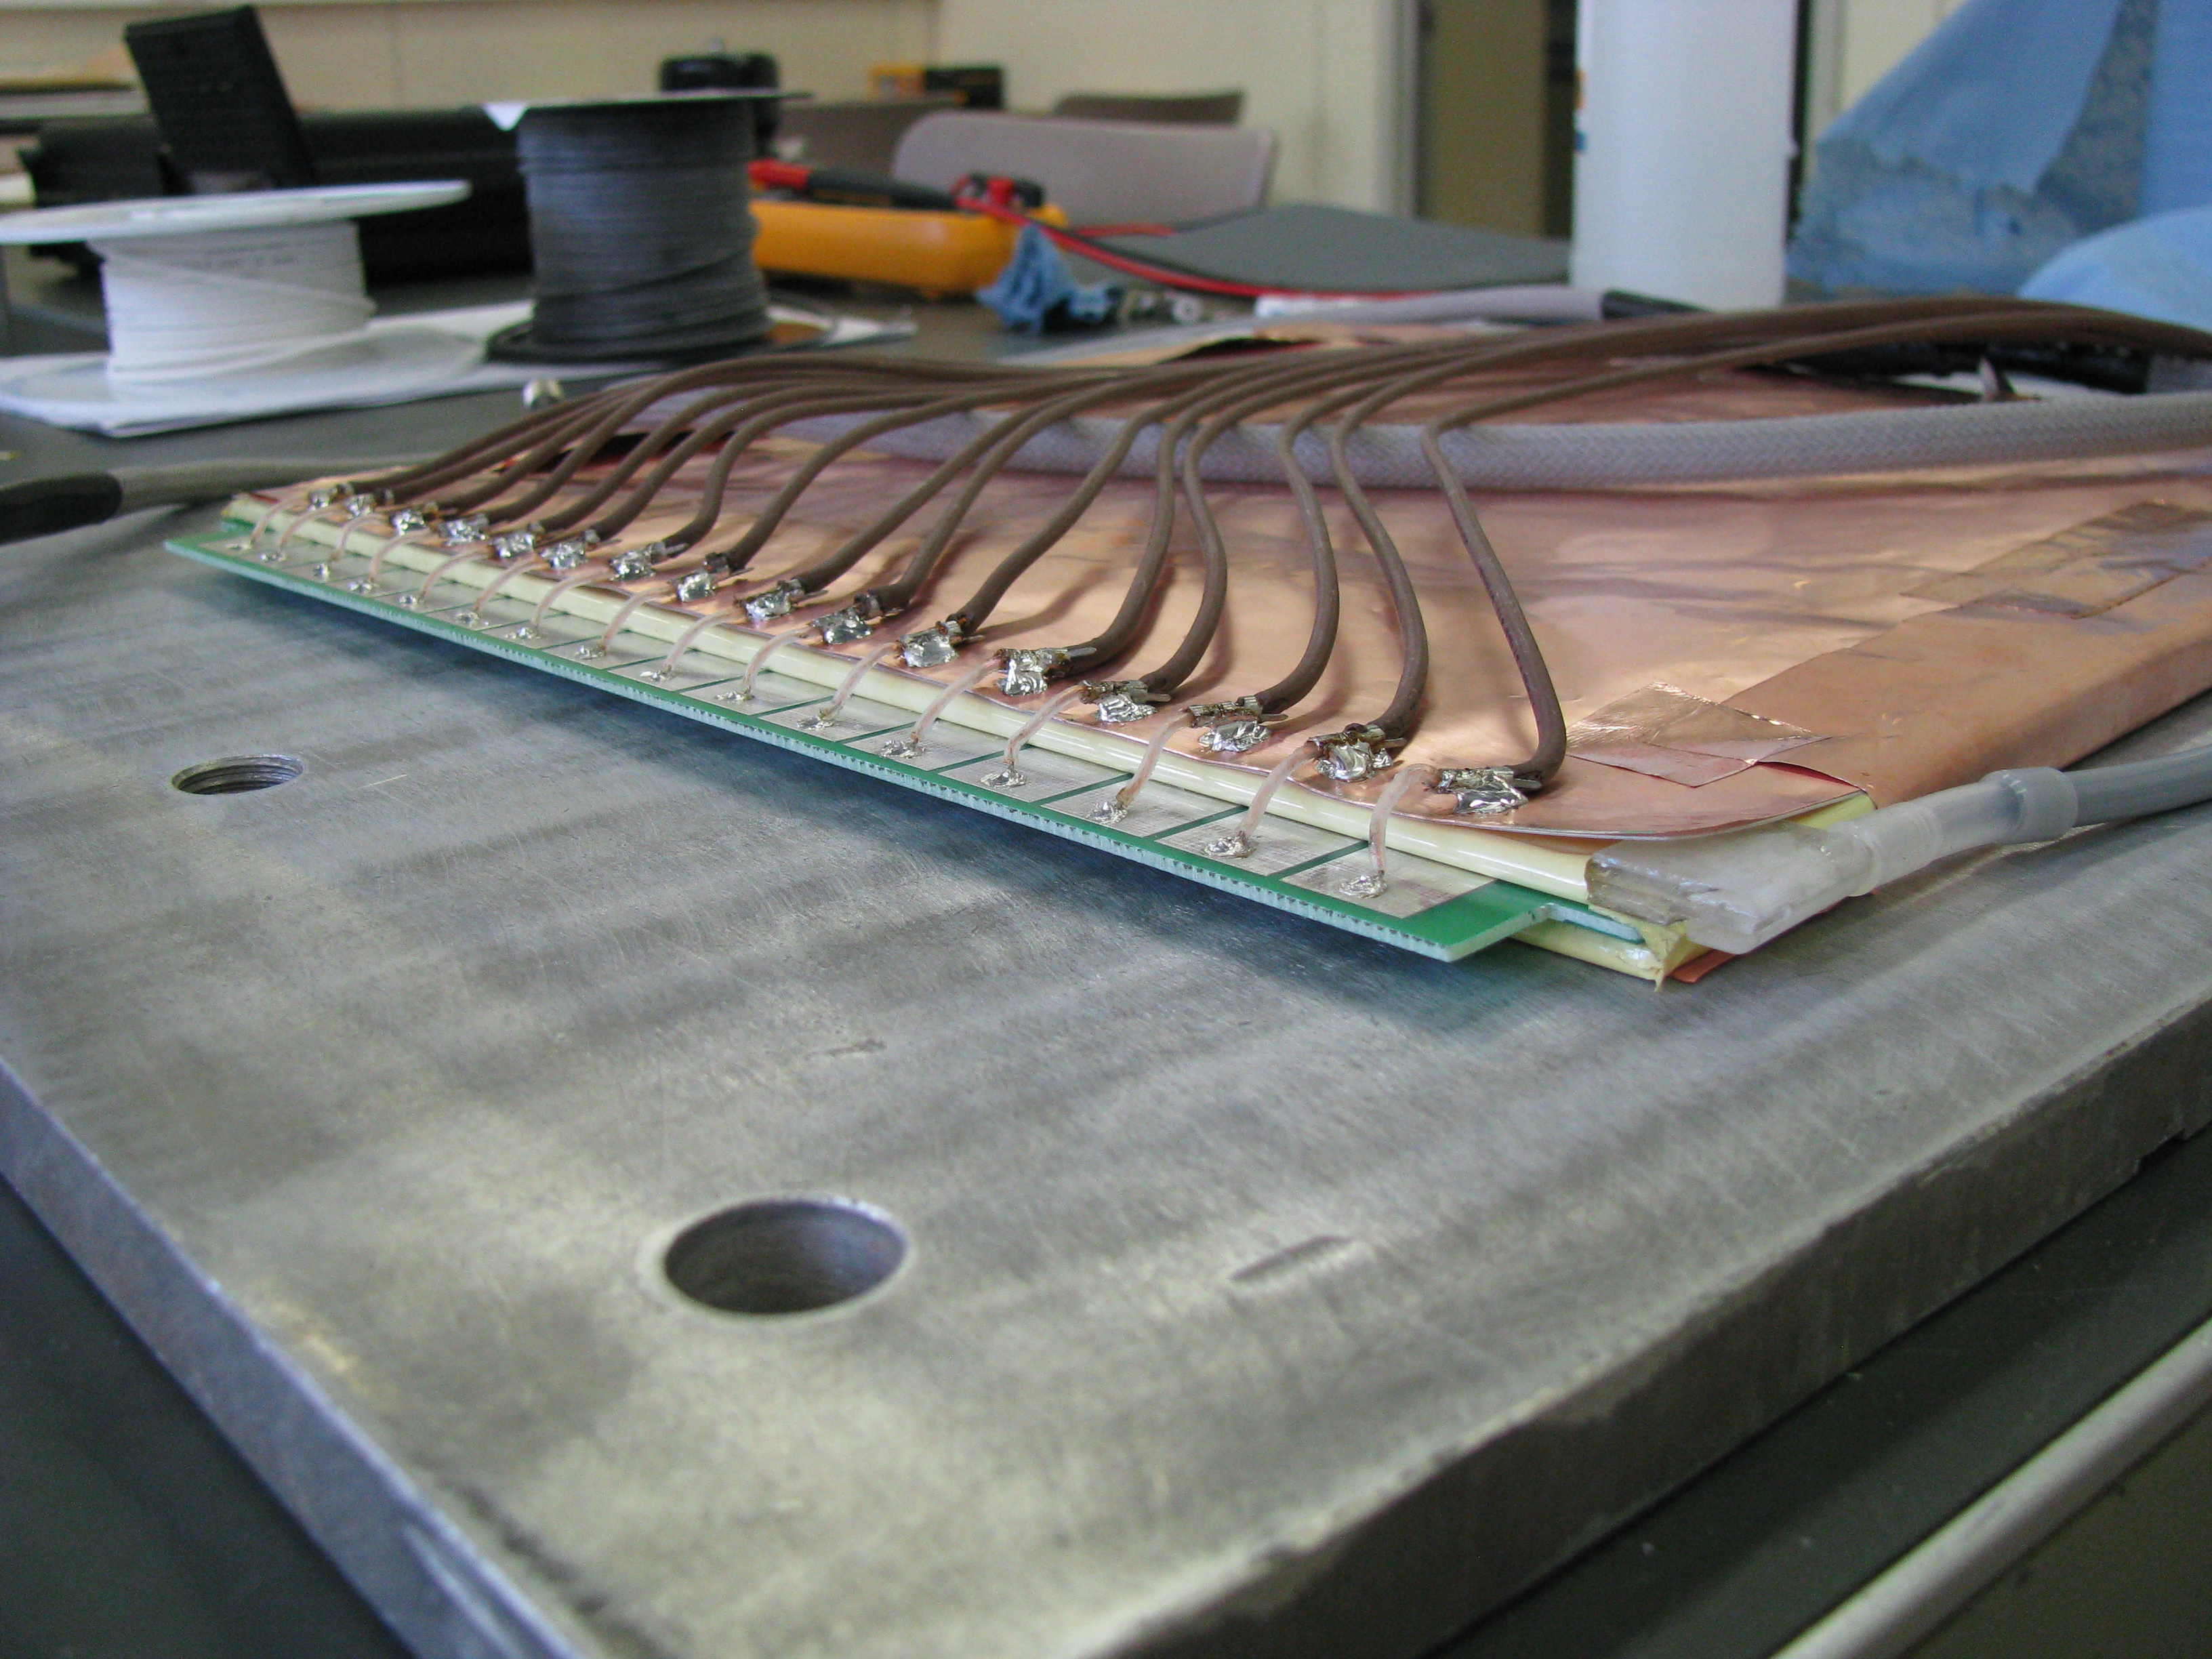
\includegraphics[width = .9\linewidth]{fig/chapt6/gRPC-faraday.JPG}
			\caption{\label{fig:UGent-gRPC-pictures:B}}
		\end{subfigure}
		\begin{subfigure}{\linewidth}
		    \centering
			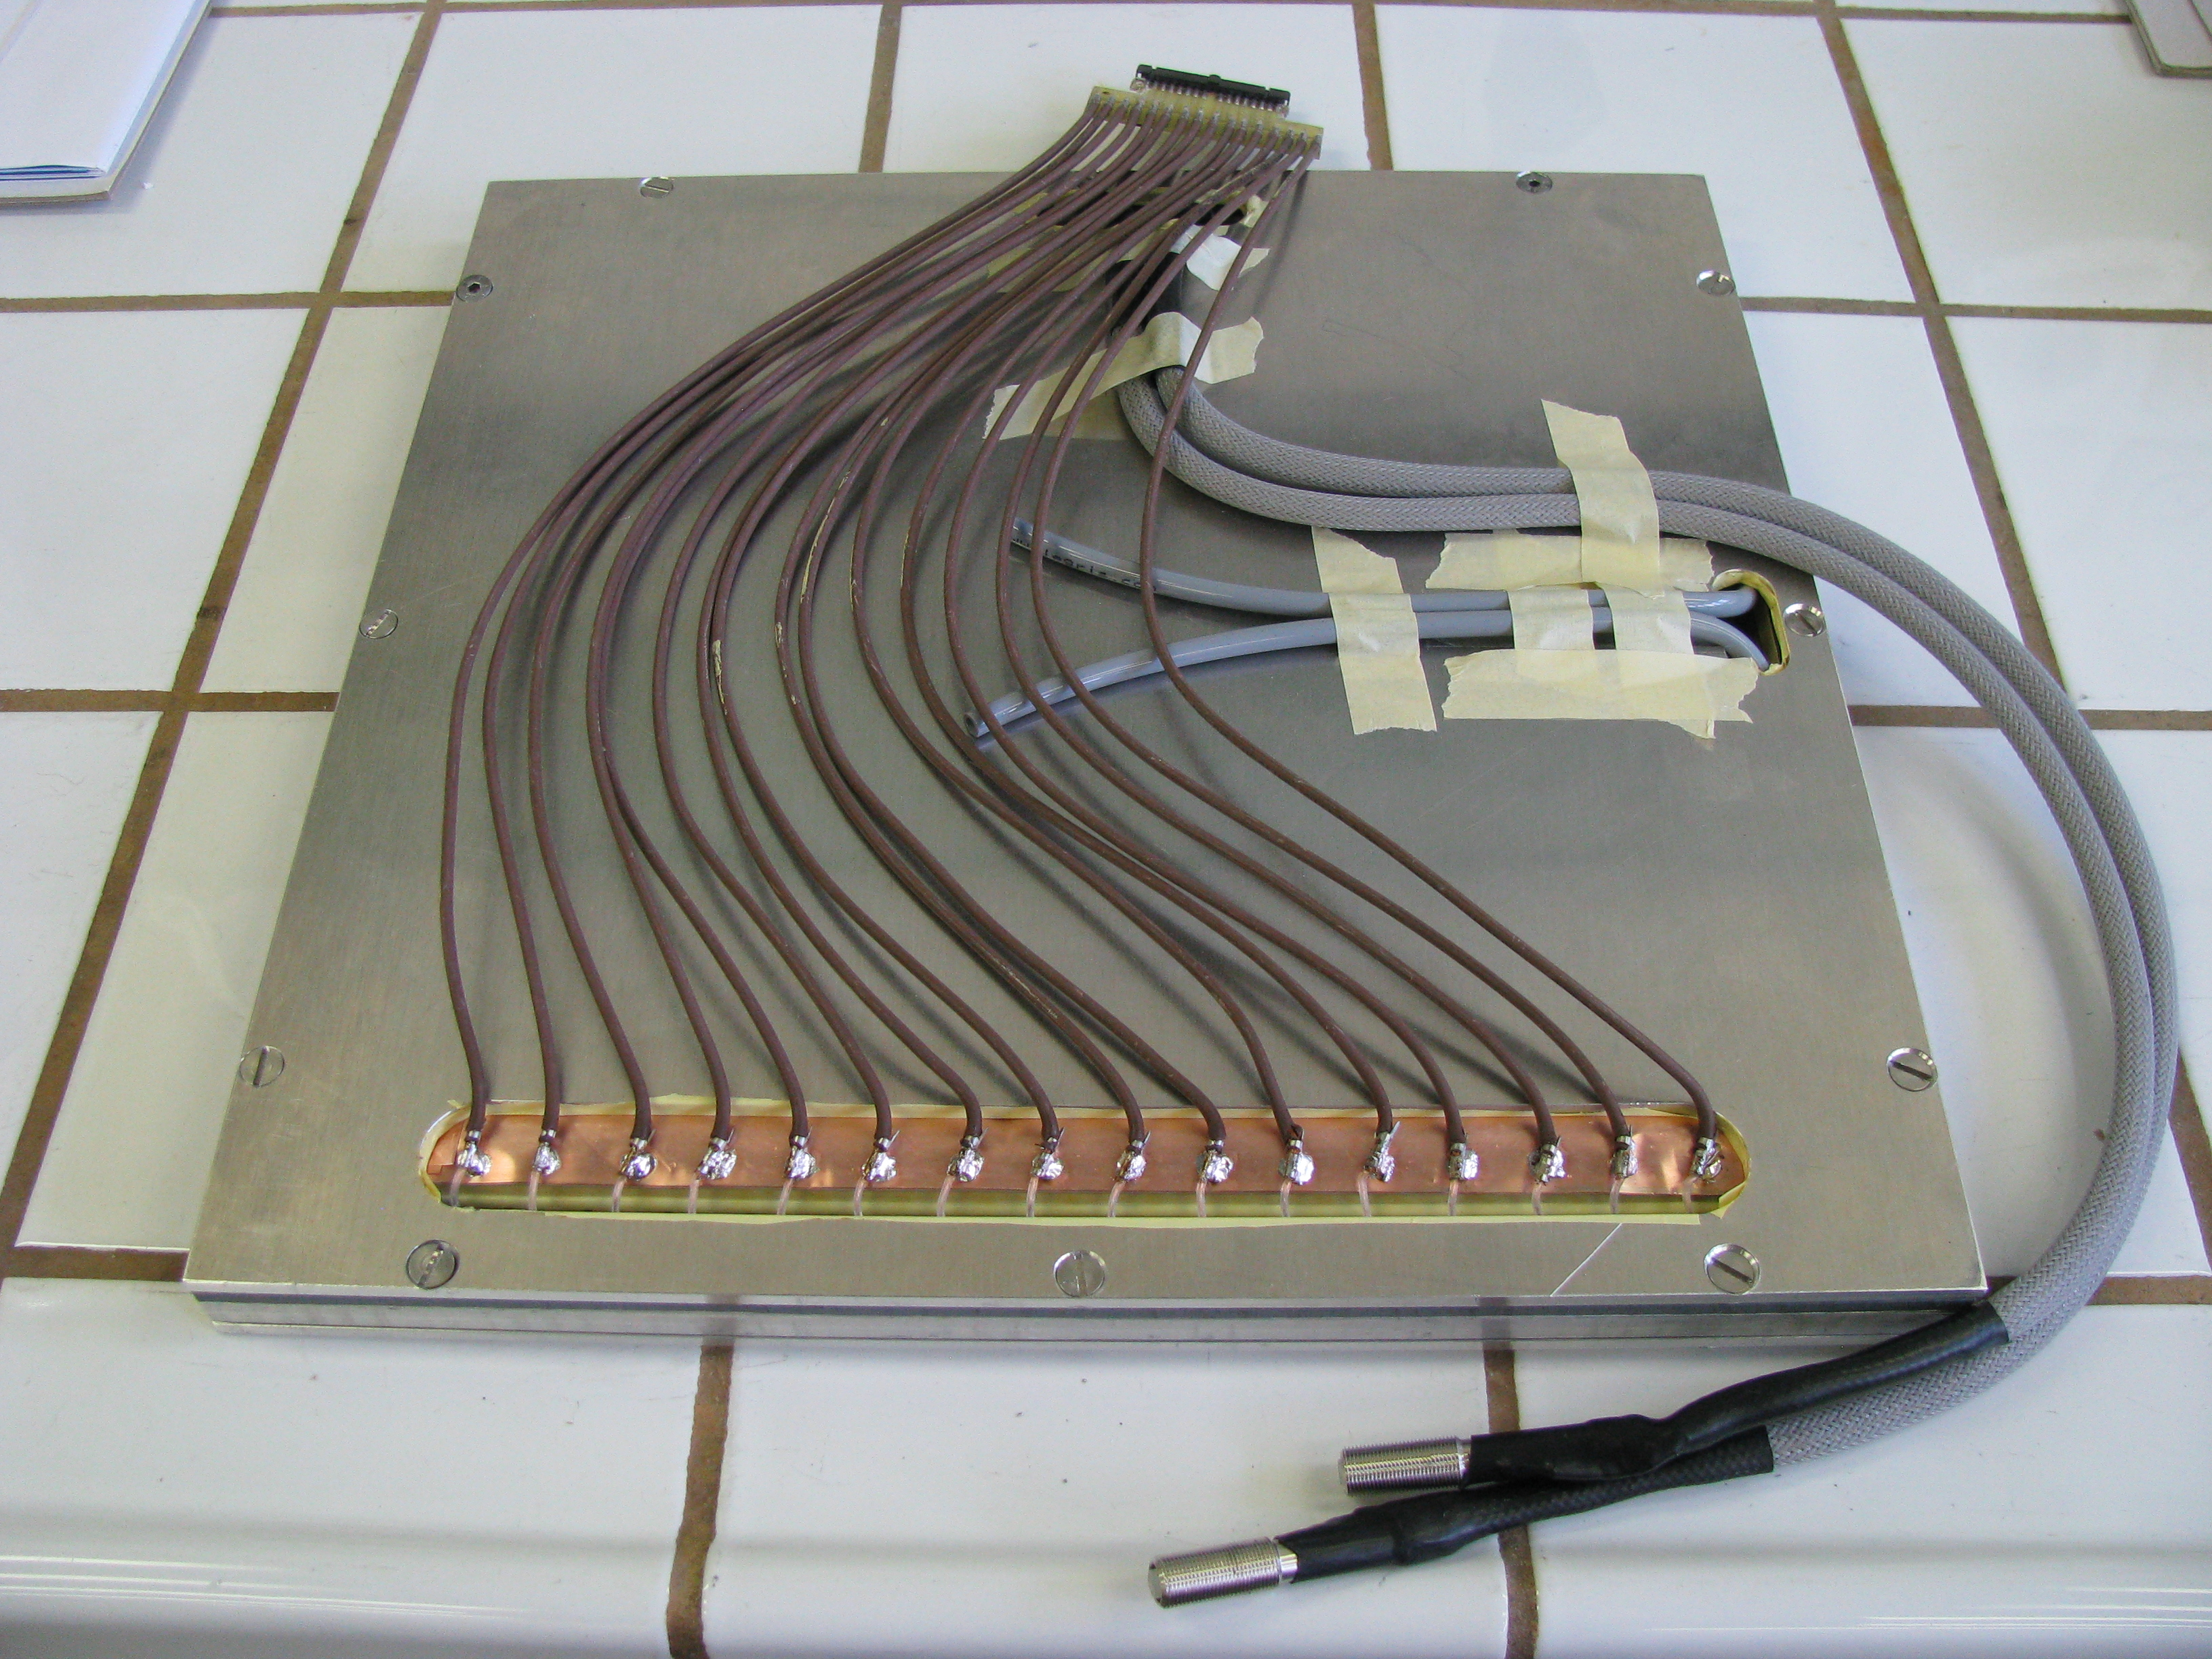
\includegraphics[width = .45\linewidth]{fig/chapt6/gRPC-case.JPG}
			\caption{\label{fig:UGent-gRPC-pictures:C}}
		\end{subfigure}
		\caption{\label{fig:UGent-gRPC-pictures} \subref{fig:UGent-gRPC-pictures:A} Picture of one of the gaps used in the gRPC tested at CERN. \subref{fig:UGent-gRPC-pictures:B} Both gaps with their read-out panel are placed into a faraday made out of copper. \subref{fig:UGent-gRPC-pictures:C} The faraday cage containing the double-gap gRPC is finally placed into its aluminium case.}
    \end{figure}

	\begin{figure}[H]
		\centering
		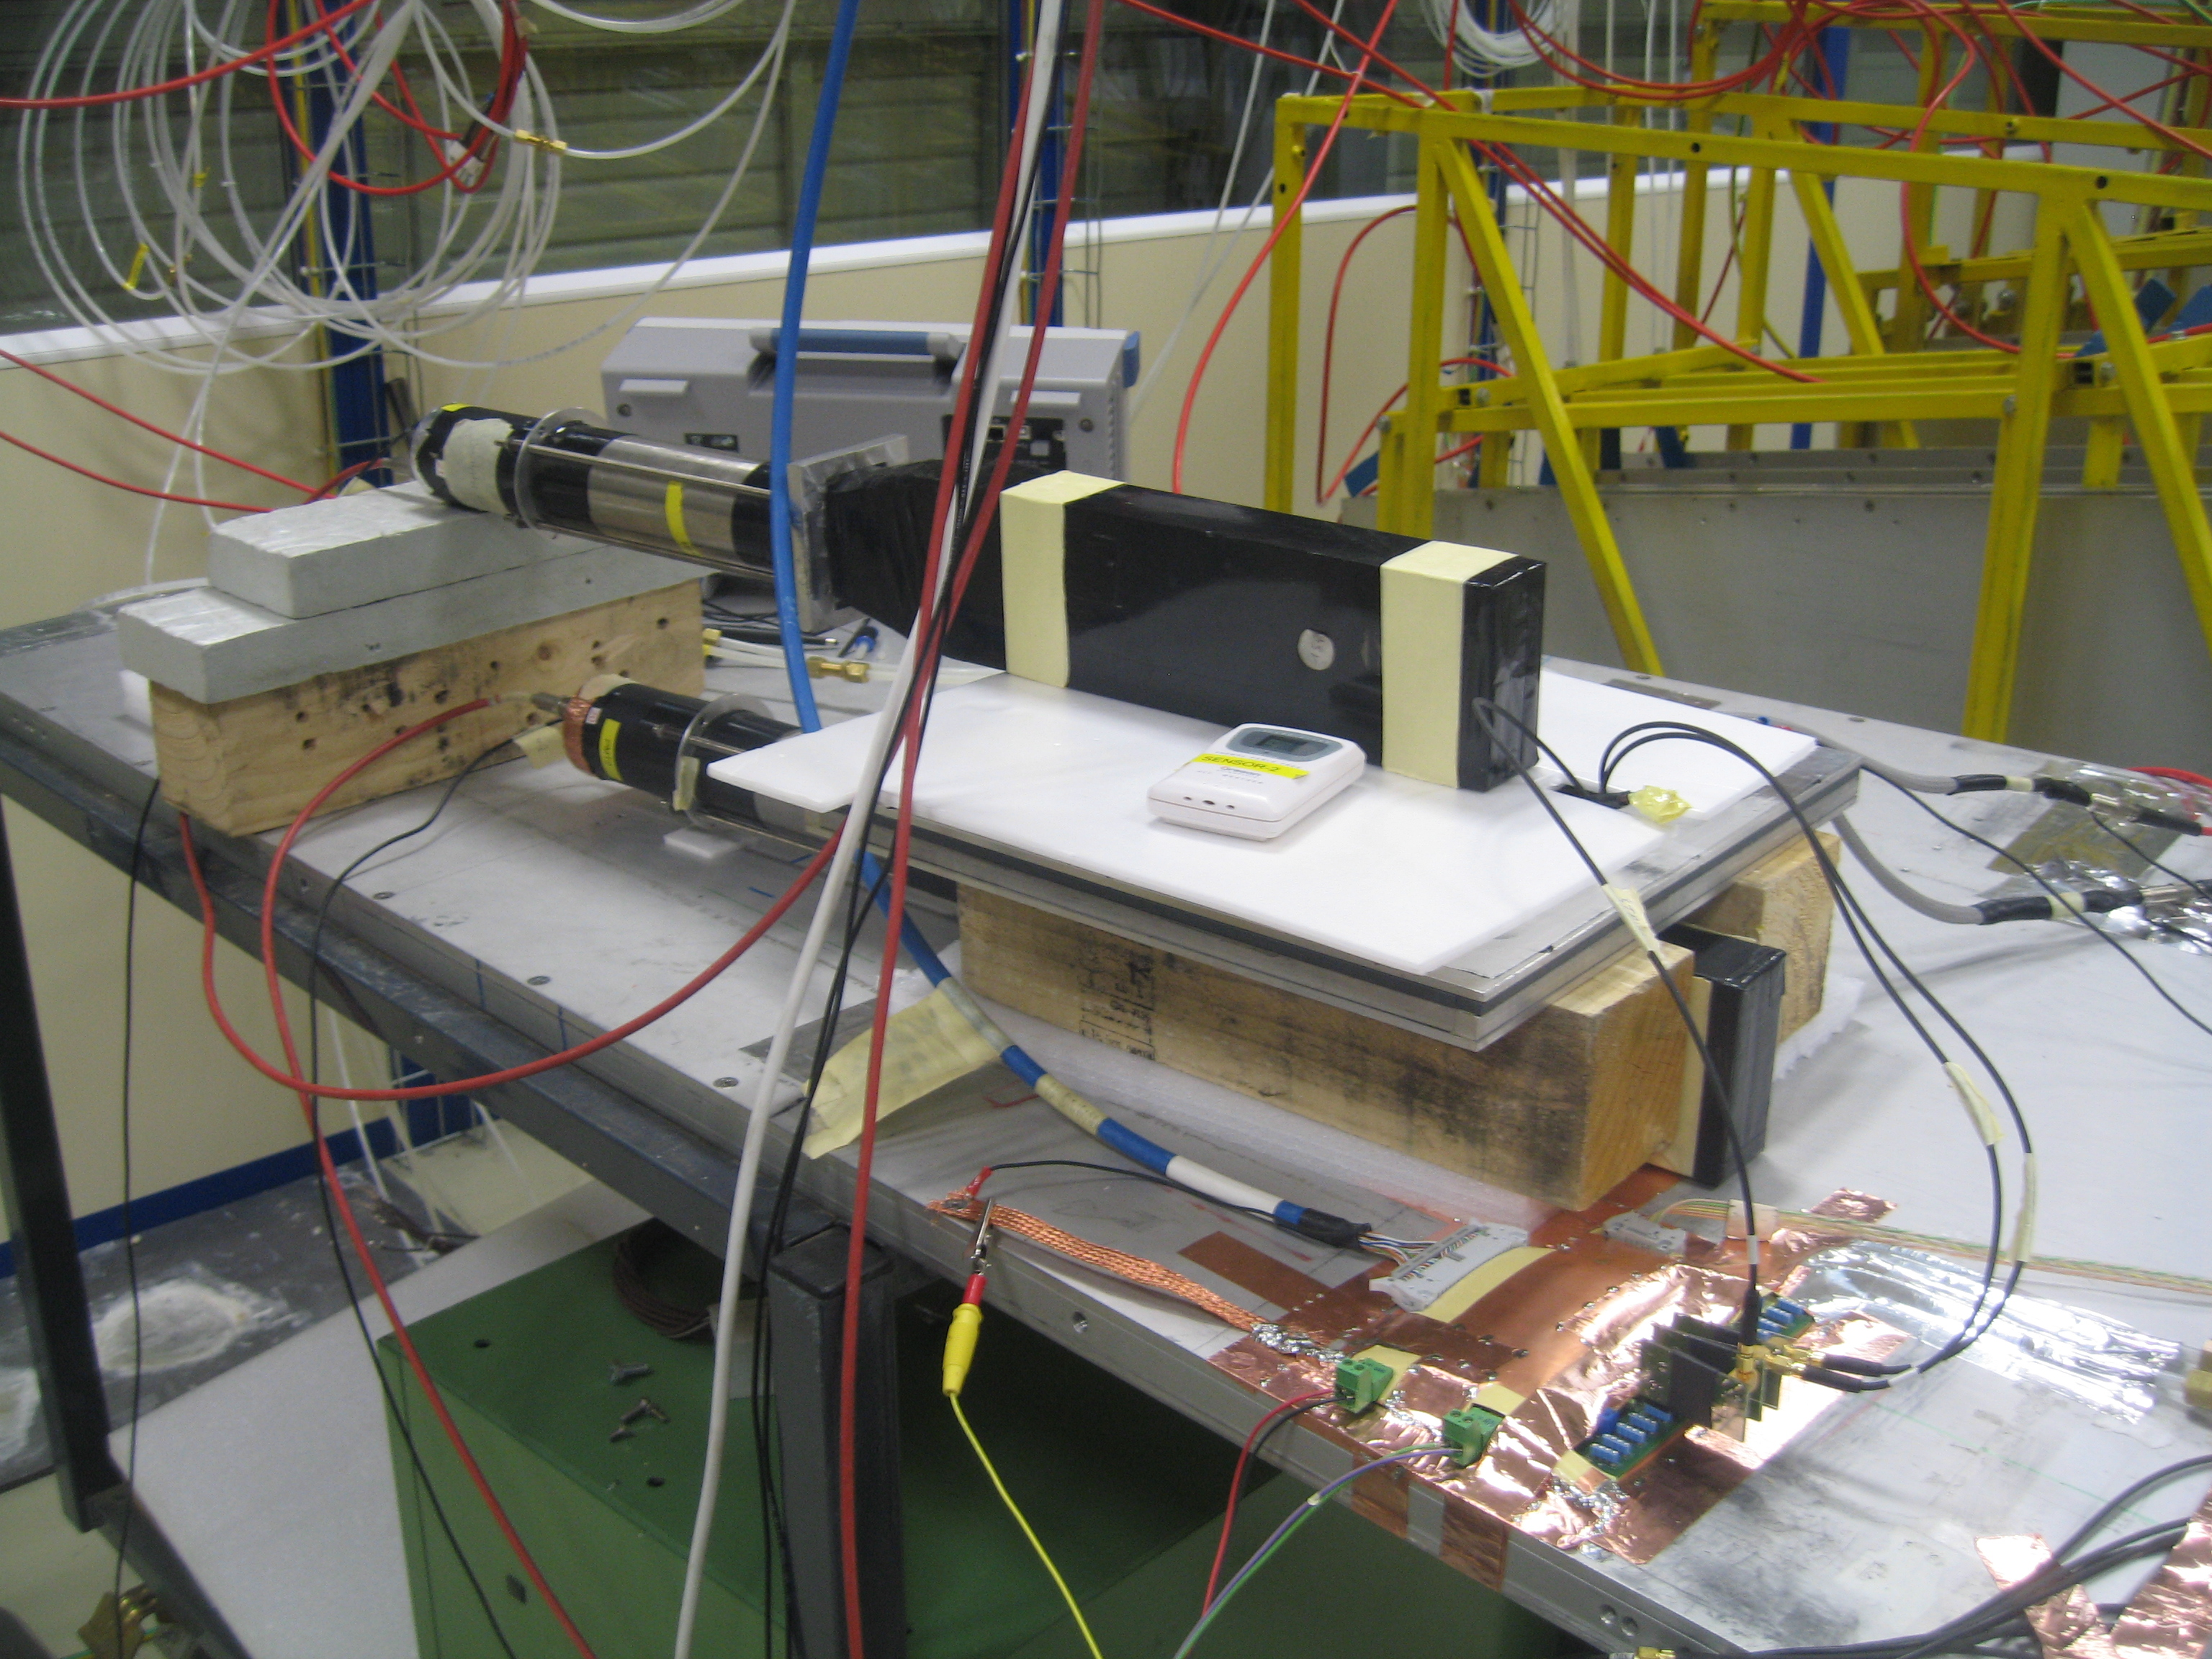
\includegraphics[width=.6\linewidth]{fig/chapt6/Setup_ATLAS_gRPC.JPG}
		\caption{\label{fig:Setup-INFN-gRPC} Experimental setup used to test the INFN preamplifier mounted on the CMS like FEB with the glass RPC build by Ghent.}
	\end{figure}
    
    Thanks to the activities ongoing for the preparation of the CMS RPC experiment taking place at GIF++ and detailed in Chapter~\ref{chapt5}, a first prototype of DAQ software was available to automate the data tacking process. Thanks to this early version of the software, the pulse processing was made more simple. The three channels connected to the preamplifiers were sent directly into a V1190A TDC manufactured by CAEN. The trigger was provided by the same trigger pulse processing described in Figure~\ref{fig:Pulse-Processing-904}. The output of the coincidence of both scintillators was sent into the \textit{TRIGGER} input of the TDC. The communication with the computer was done thanks to a V1718 module. More details on the DAQ can be found in Appendix~\ref{app1}. Contrary to the data now collected at GIF++, the output of the first DAQ script consisted in a simple text file using a format described in Source Code~\ref{text:data}. The analysis is then performed using a loop through the data file.
    
    \begin{code}
    \vspace{5mm}
    \begin{textcode}
Evt0	nHits
ChHit1	THit1
ChHit2	THit2
ChHit3	THit3
ChHit4	THit4
ChHit5	THit5
...
Evt1	nHits
ChHit1	THit1
ChHit2	THit2
ChHit3	THit3
...
    \end{textcode}
	\captionof{listing}{Description of the format used to store the data collected during the experiment aiming at testing the INFN electronics with a gRPC built by Ghent. For each received trigger in the TDC module, an event is created. A first line containing two columns is written in the output file with the event number \textinline{EvtX} and the recorded number of hits  \textinline{nHits}. This line is directly followed by the list of hits in each channel \textinline{ChHitX} and their corresponding time stamp \textinline{THitX} organized into two columns.}
	\label{text:data}
	\vspace{5mm}
    \end{code}
    
    The results of the experiment with the gRPC are provided in Figure~\ref{fig:INFN-gRPC} and Table~\ref{tab:INFN-gRPC}. The efficiency of the detector reaches 95\% at working voltage, indicating that such a detector using electrodes composed of several glued pieces can be an option for the future of RPC technologies. The benefits of the preamplifiers is once again visible through the huge efficiency shift towards lower voltages. The shift reaches almost \SI{470}{V} for thresholds lower than \SI{6}{fC}.\\
    The cluster size also shows a shift but its value suddenly decreases after \SI{5.4}{kV}. After a rise above 2, the cluster size drops when the detector reaches the plateau. A first idea to explain this phenomenon would be to check the cluster algorithm to make sure that it is not biased and does not introduce a fake split of the clusters due to arbitrarily strict selection rules. Clusters are always made of neighbour strips getting a hit within a certain time window. In the algorithm written to analyse the data, it is required for the maximum time difference between the earliest hit and the latest hit in a cluster to be smaller than \SI{10}{ns}. Physically, assuming of drift velocity of the electrons in the gas of the order of \SI{0.1}{mm/ns}~\cite{DEURQUIJO2009}, the growth of an avalanche only takes a few \si{ns}. This effect is visible in Figure~\ref{fig:avalanche-growth:A} in which the maximum time difference has been artificially increased to \SI{300}{ns}. The peak reveals that the avalanches are not expected to grow over a time period longer than \SI{10}{ns}. No peak emerges at time differences longer than \SI{10}{ns} indicating that the choice of a short time development within the algorithm was justified. This conclusion is supported by Figure~\ref{fig:avalanche-growth:B} in which the evolution of the reconstructed cluster size with increasing maximum time difference shows no effect.
    
\newpage
    
    \begin{figure}[H]
		\begin{subfigure}{.5\linewidth}
		    \centering
			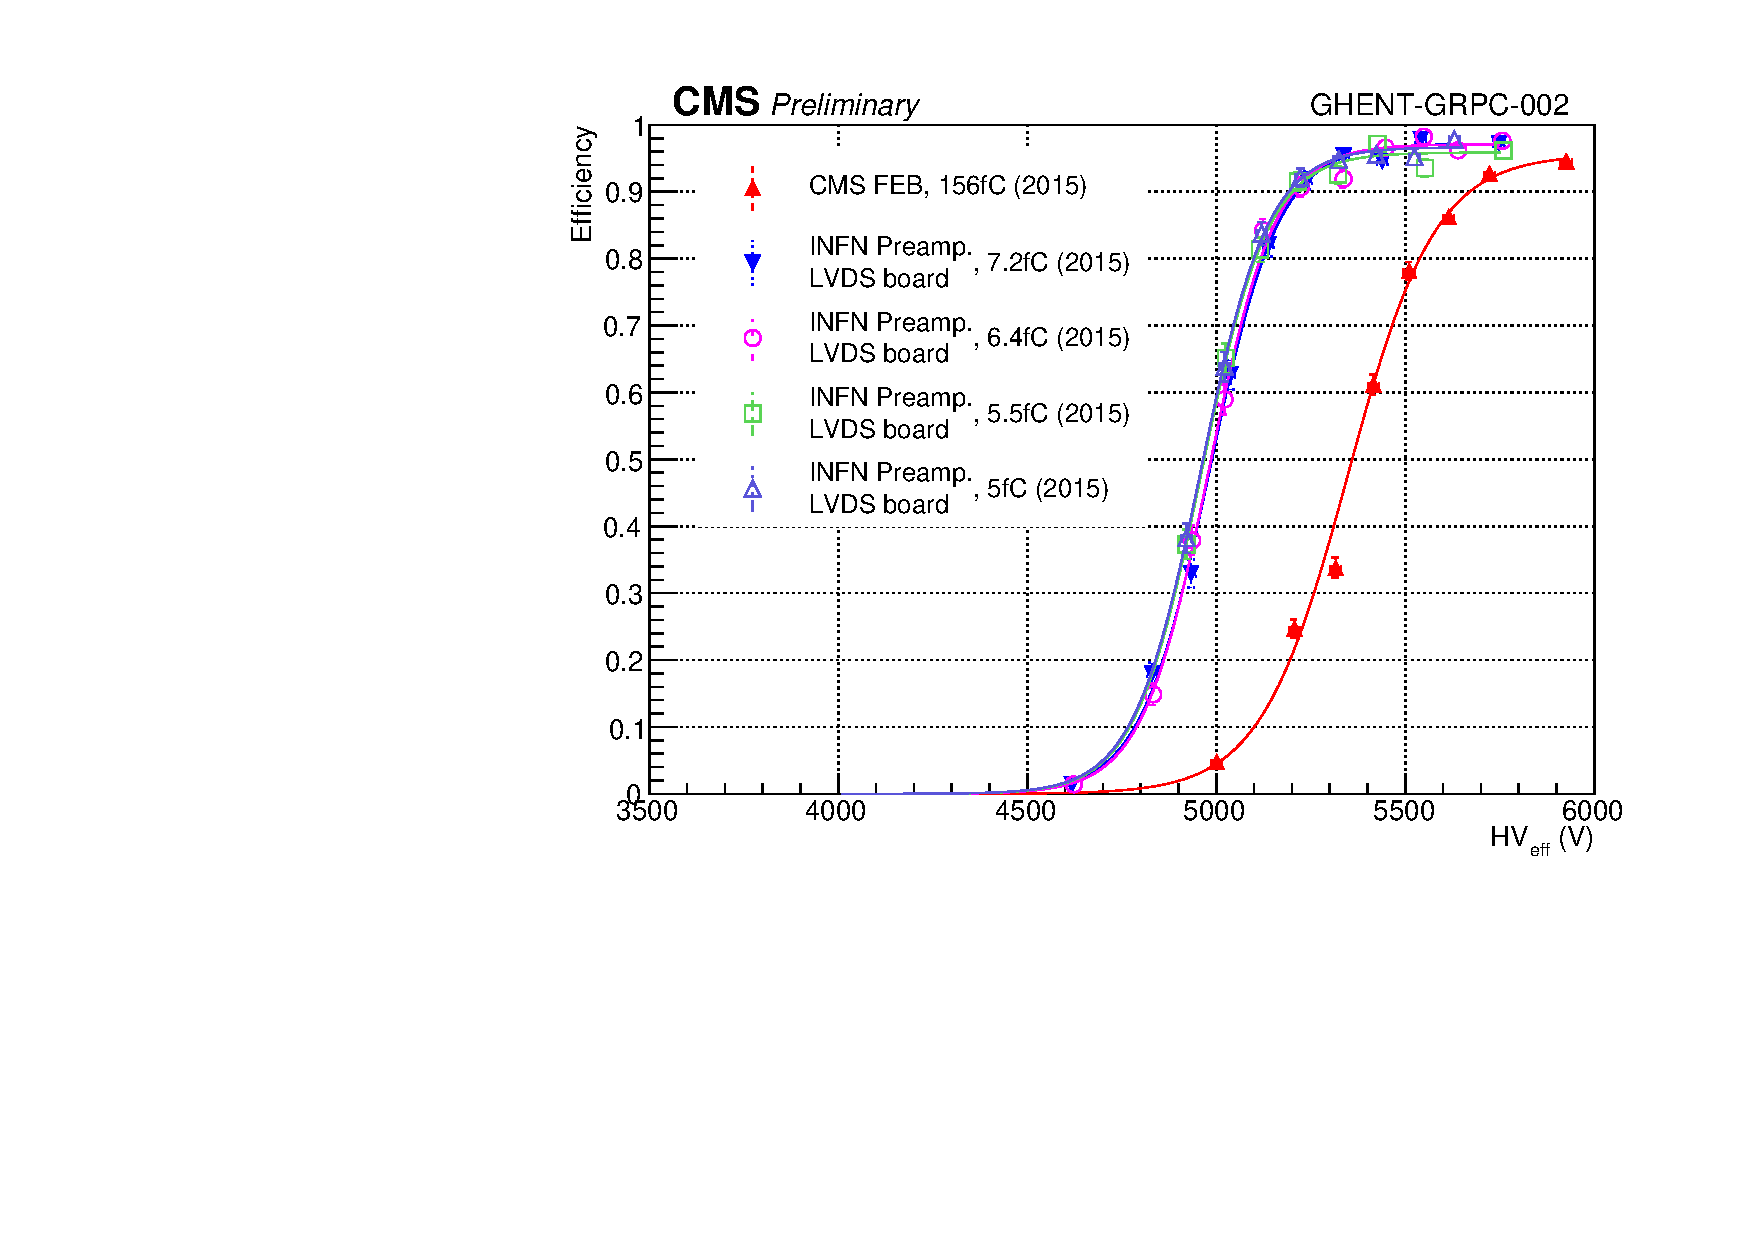
\includegraphics[width=\linewidth]{fig/chapt6/gRPC-INFN-LVDS-Eff-Shift.pdf}
			\caption{\label{fig:INFN-gRPC:A}}
		\end{subfigure}
		\begin{subfigure}{.5\linewidth}
		    \centering
			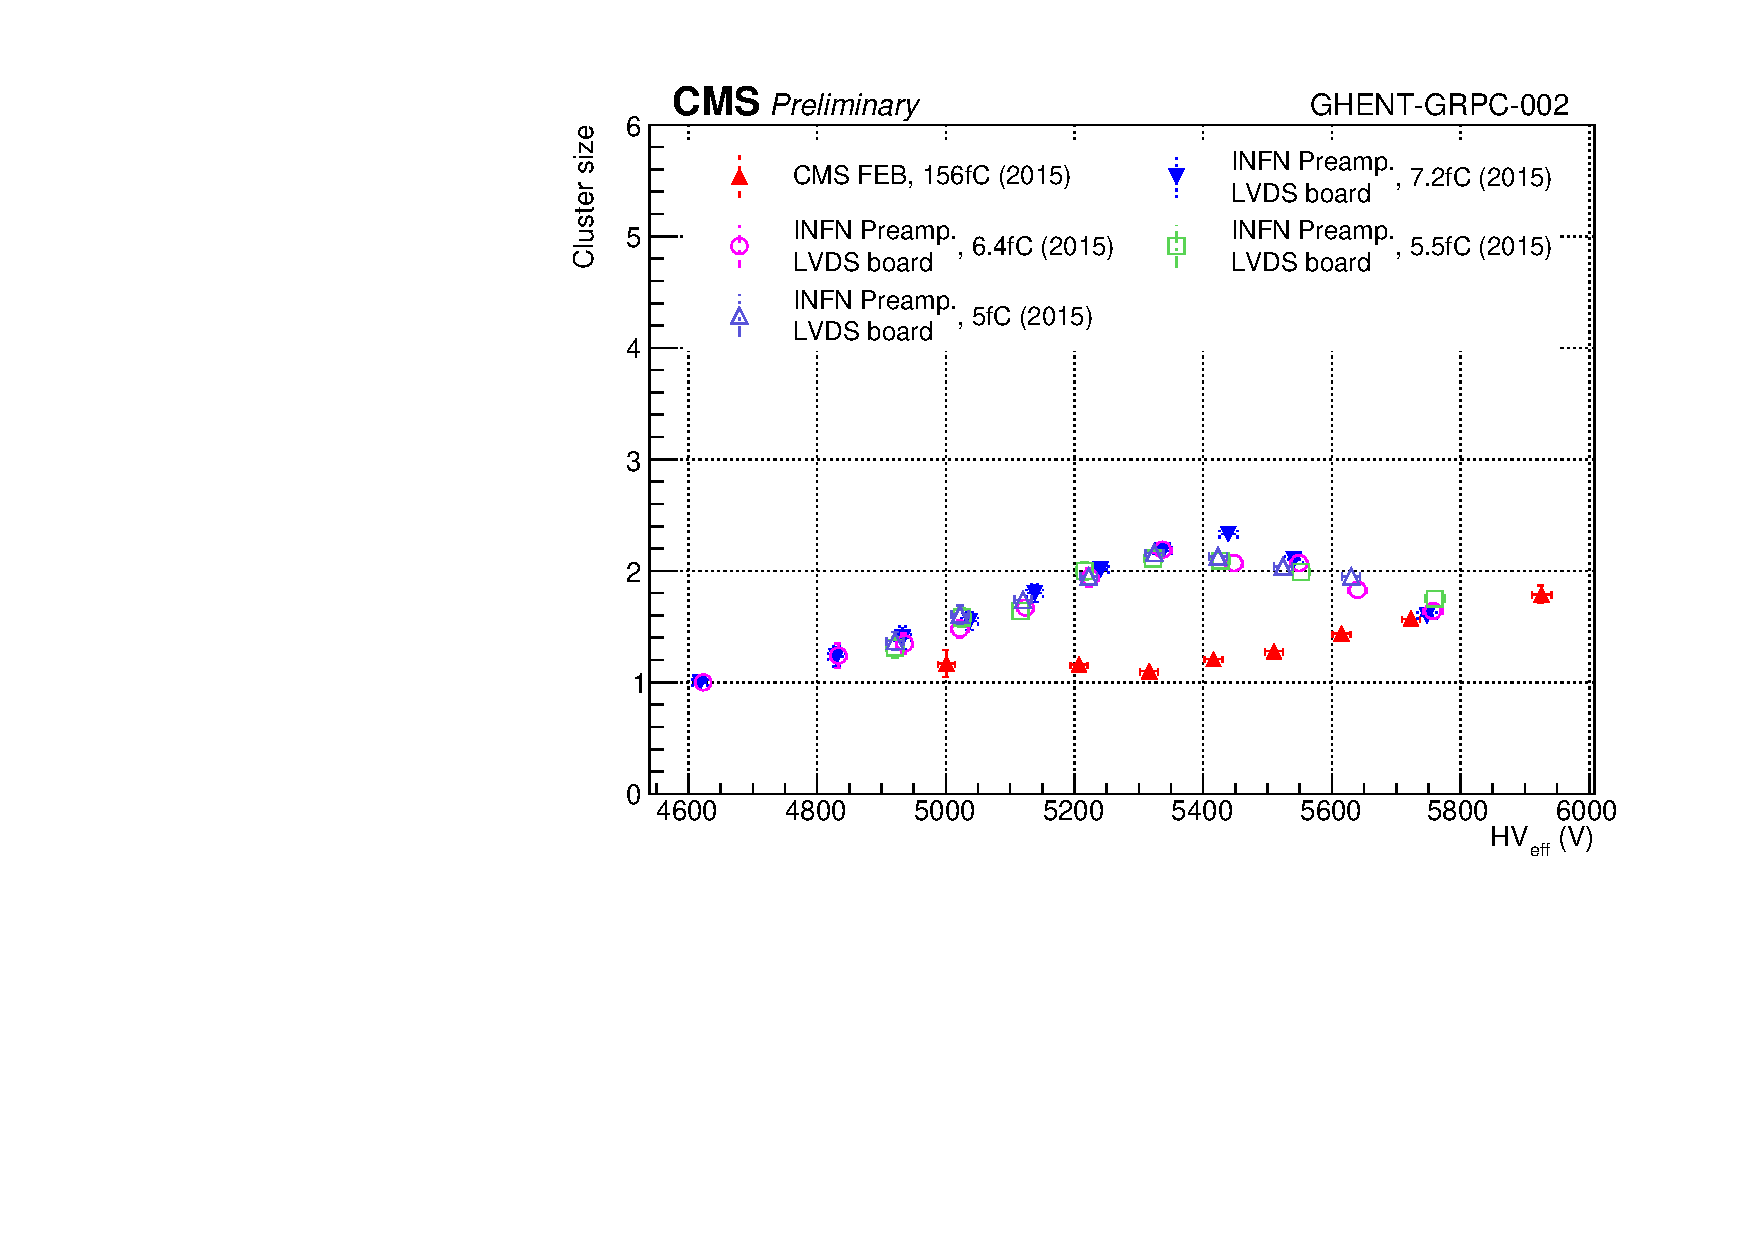
\includegraphics[width = \linewidth]{fig/chapt6/gRPC-INFN-LVDS-ClS-Shift.pdf}
			\caption{\label{fig:INFN-gRPC:B}}
		\end{subfigure}
		\begin{subfigure}{\linewidth}
		    \centering
			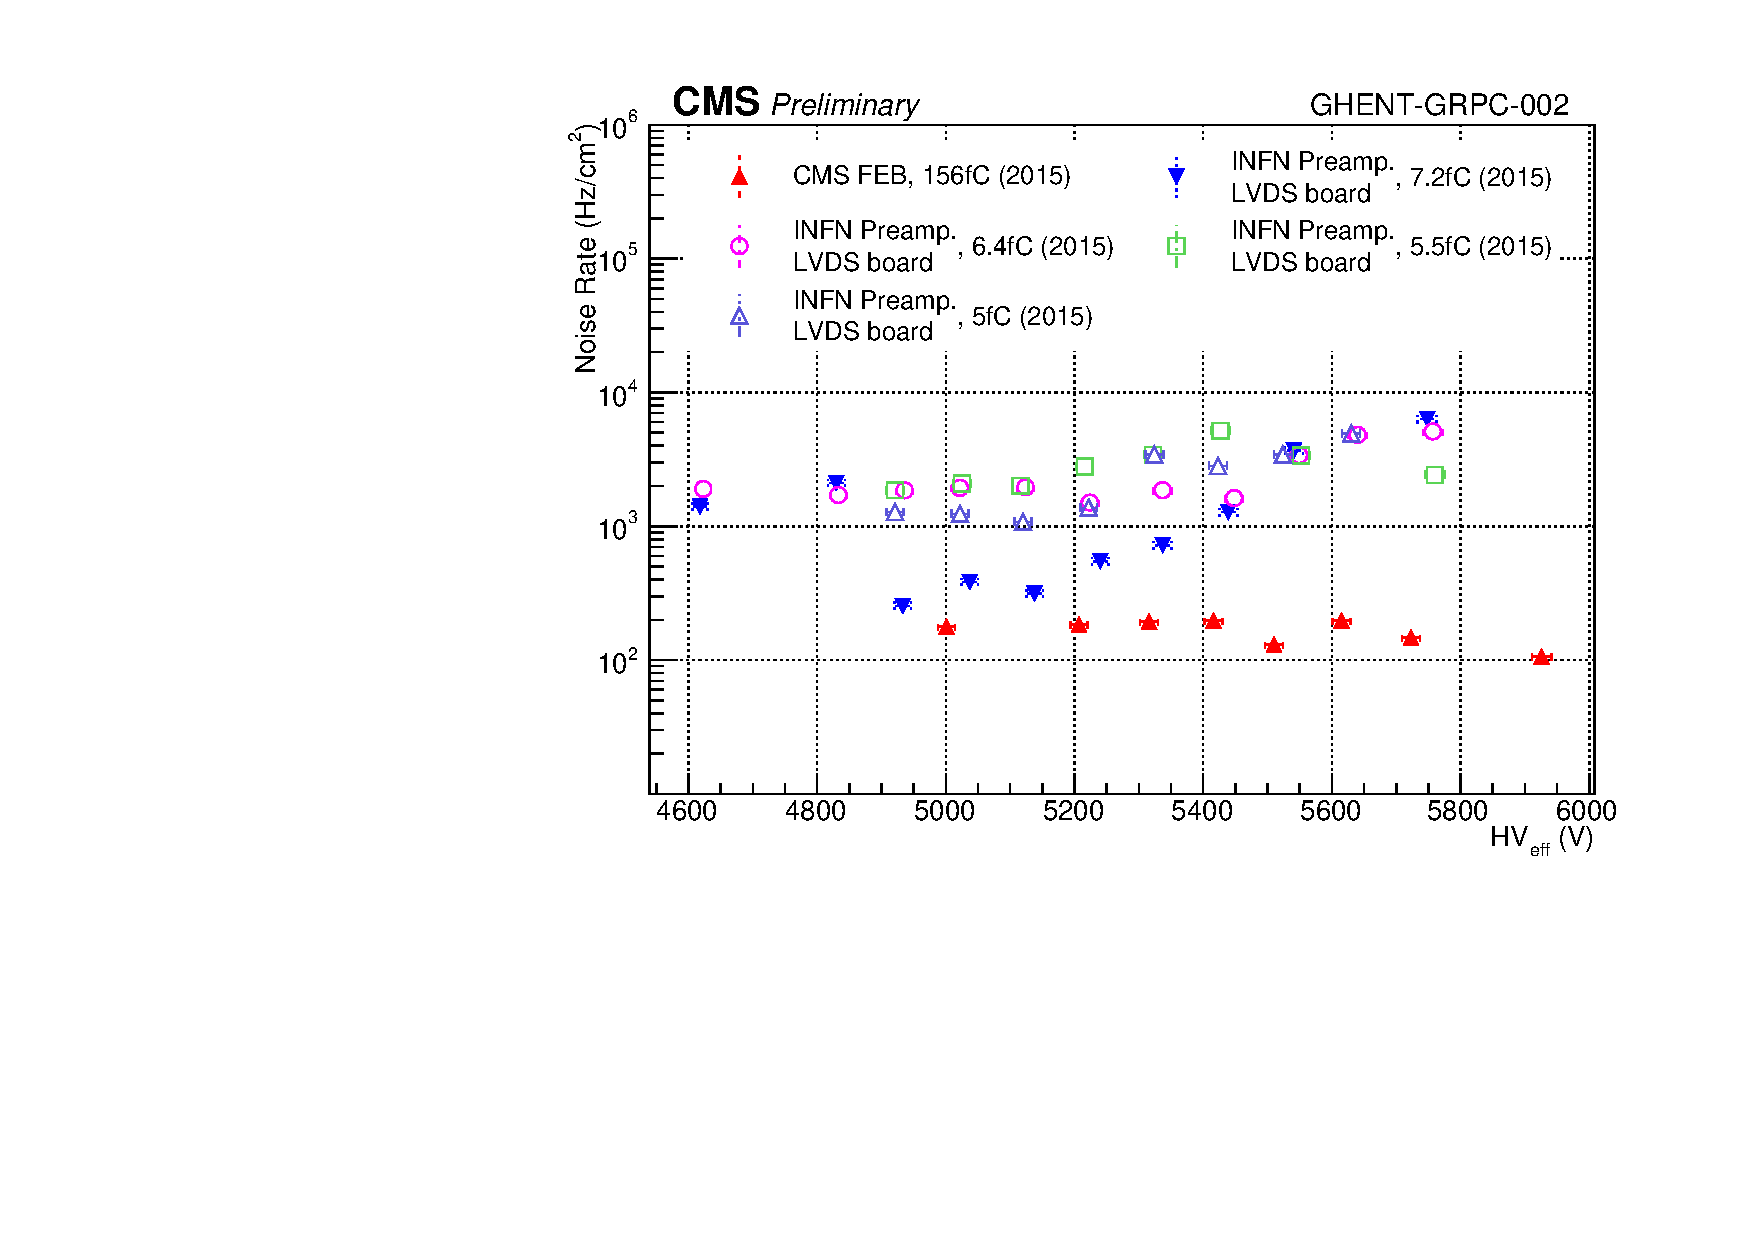
\includegraphics[width = .5\linewidth]{fig/chapt6/gRPC-INFN-LVDS-Rate-Shift.pdf}
			\caption{\label{fig:INFN-gRPC:C}}
		\end{subfigure}
		\caption{\label{fig:INFN-gRPC} Efficiency~\subref{fig:INFN-gRPC:A}, cluster size~\subref{fig:INFN-gRPC:B} and noise rate per unit area~\subref{fig:INFN-gRPC:C} of the Ghent gRPC detector tested with the standard CMS FEBs (red) and with the INFN preamplifier mounted onto the CMS FEB at different thresholds (blue, pink, green and purple).}
	\end{figure}
	
	\begin{table}[H]
		\caption{\label{tab:INFN-gRPC} Results of the sigmoid fit (Equation~\ref{eq:Sigmoid}) performed on the data presented in Figure~\ref{fig:INFN-gRPC:A}. The working point and its corresponding efficiency are computed using Equations~\ref{eq:Sigmoid} and \ref{eq:KneeWP}.}
		\footnotesize
		\begin{tabular}{|c|c|c|c|c|c|}
			\hline
Data & $\epsilon_{max}$ & $\lambda$ ($\cdot$\Ord{-2} \si{V^{-1}}) & $HV_{50}$ (\si{V}) & $\epsilon_{WP}$ & $HV_{WP}$ (\si{V}) \\ 
			\hline
CMS FEB, 143fC (2015)      & $0.956 \pm 0.007$ & $0.86 \pm 0.04$ & $5349 \pm 8$  & $0.94 \pm 0.01$ & $5839 \pm 23$\\ 
			\hline
INFN/CMS FEB, 7.2fC (2015) & $0.972 \pm 0.006$ & $1.09 \pm 0.06$ & $4983 \pm 8$  & $0.96 \pm 0.01$ & $5403 \pm 22$\\ 
			\hline
INFN/CMS FEB, 6.4fC (2015) & $0.971 \pm 0.005$ & $1.13 \pm 0.06$ & $4981 \pm 8$  & $0.96 \pm 0.01$ & $5391 \pm 22$\\ 
			\hline
INFN/CMS FEB, 5.5fC (2015) & $0.959 \pm 0.006$ & $1.13 \pm 0.11$ & $4960 \pm 11$ & $0.95 \pm 0.02$ & $5371 \pm 37$\\ 
			\hline
INFN/CMS FEB, 5fC (2015)   & $0.967 \pm 0.006$ & $1.12 \pm 0.11$ & $4959 \pm 11$ & $0.96 \pm 0.02$ & $5371 \pm 38$\\ 
			\hline
		\end{tabular}
	\end{table}
	
	\begin{figure}[H]
		\begin{subfigure}{.5\linewidth}
		    \centering
			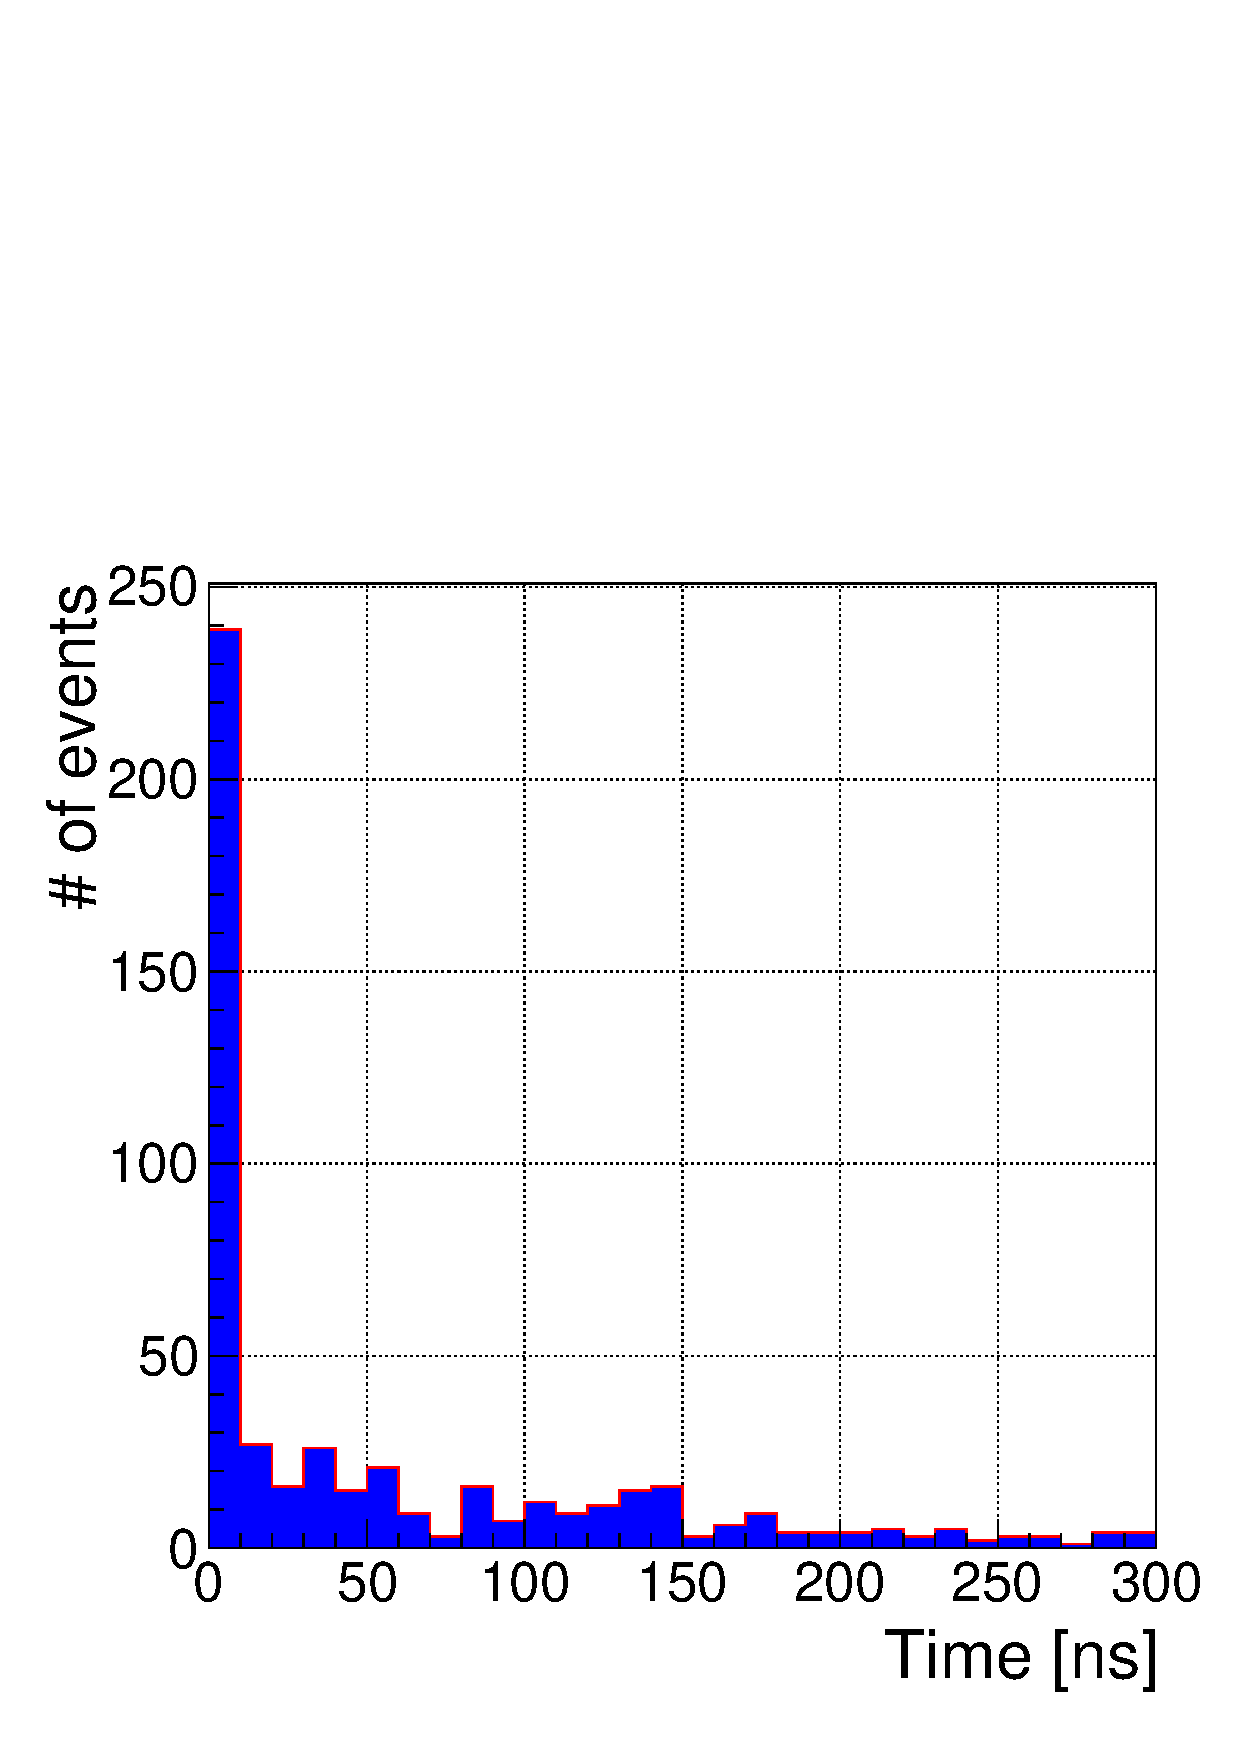
\includegraphics[width=\linewidth]{fig/chapt6/Muon-Avalanche-Growth-gRPC-INFN.pdf}
			\caption{\label{fig:avalanche-growth:A}}
		\end{subfigure}
		\begin{subfigure}{.5\linewidth}
		    \centering
			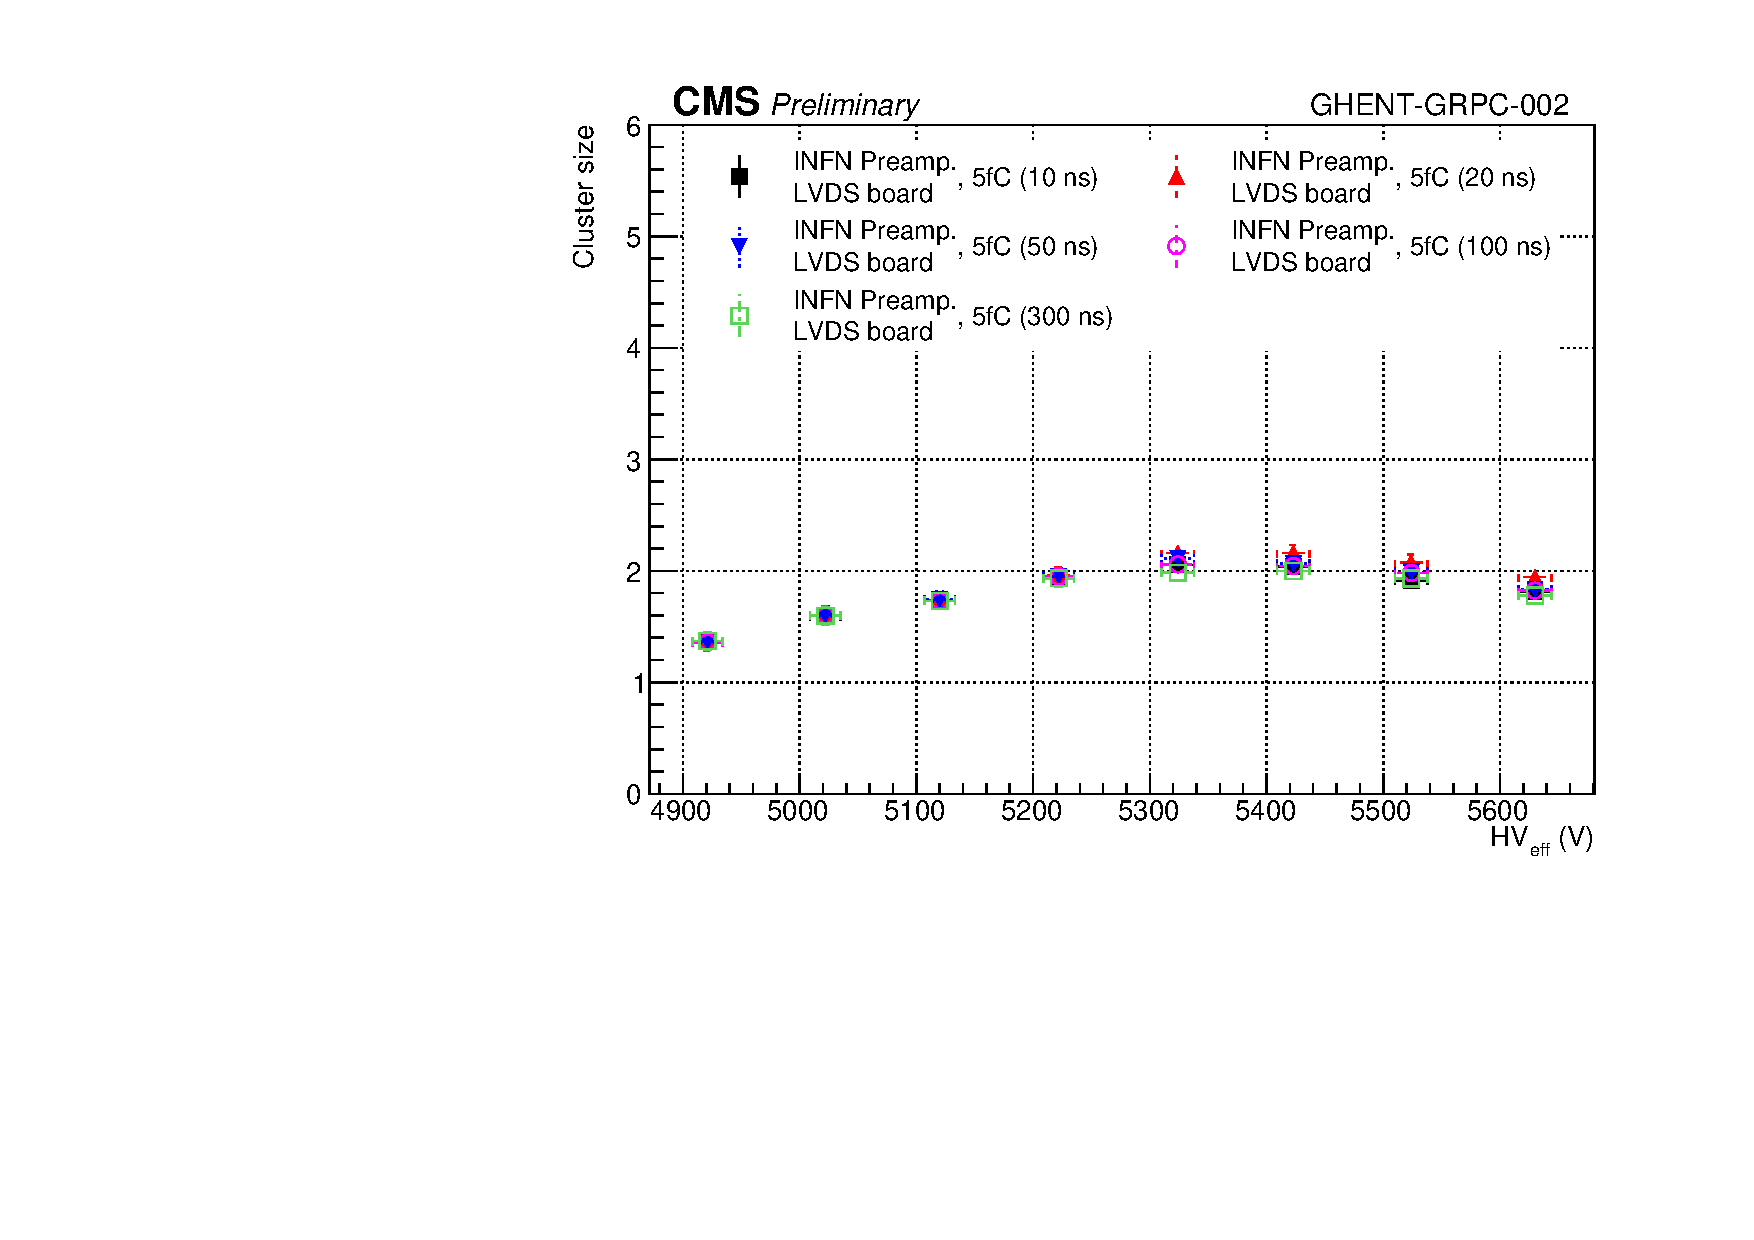
\includegraphics[width = \linewidth]{fig/chapt6/gRPC-INFN-LVDS-ClS-Study.pdf}
			\caption{\label{fig:avalanche-growth:B}}
		\end{subfigure}
		\caption{\label{fig:avalanche-growth} \subref{fig:avalanche-growth:A} Time difference between the first and last hit composing a cluster in the gRPC. The maximum time difference is set to \SI{300}{ns}. \subref{fig:avalanche-growth:B} Variation of the reconstructed average cluster size as a function of the time constraint used in the algorithm.}
	\end{figure}
	
	Due to the available number of channels, the cluster size is limited to 3. It is reasonable to assume that this only is the cause of the fall of cluster size beyond \SI{5.4}{kV}. Indeed looking closely at both Figure~\ref{fig:cluster-size-1D} and Figure~\ref{fig:cluster-size-2D}, the link between increasing HV and decreasing cluster size can be understood. On the one hand, Figure~\ref{fig:cluster-size-1D} indicates that the cluster size features at first a maximum at 1. The maximum moves then from 1 to 3 over the points at \SI{5120}{V}, \SI{5222}{V} and \SI{5324}{V}. Then over the last three voltage points, the bin at 2 drops to the profit of the bin at 1, the bin at 3 staying more or less stable. On the other hand, Figure~\ref{fig:cluster-size-2D} provides us more information about the localisation of the clusters among the three read-out strips. At the lowest two voltages, most of the data is contained in the central strip. At \SI{5120}{V}, the highest bin is the one corresponding to the central strip with a cluster size of 1. Already at \SI{5222}{V}, the balance changes towards the central strip with 3 strips in the clusters. At \SI{5324}{V}, even more events happen with clusters of all 3 strips while the events with a single hit in the side strips starts to increase. The number of events with clusters made of all 3 strips will not vary much anymore while the number of events with clusters made of 2 strips will decrease and the single hits in the side strips will continue rising. This information indicates that the avalanches in the gap start to get stronger. Indeed, the increase of the events containing single hits mainly increases on the side strips points to an intensification of the avalanche gain on the strip adjacent to the three channels connected to the read-out setup. Only a single hit is read-out while in reality this was the contribution of bigger avalanches. The events with clusters of size 2 tend to decrease due to the stronger gain that should normally be triggering wider avalanches. The cluster size distribution of Figure~\ref{fig:cluster-size-1D} gives the impression that the distribution is moving towards higher values but the geometrical limitation of the system due to the very low number of channels makes it impossible to measure.
	
\newpage
	
	\begin{figure}[H]
		\begin{subfigure}{.33\linewidth}
		    \centering
			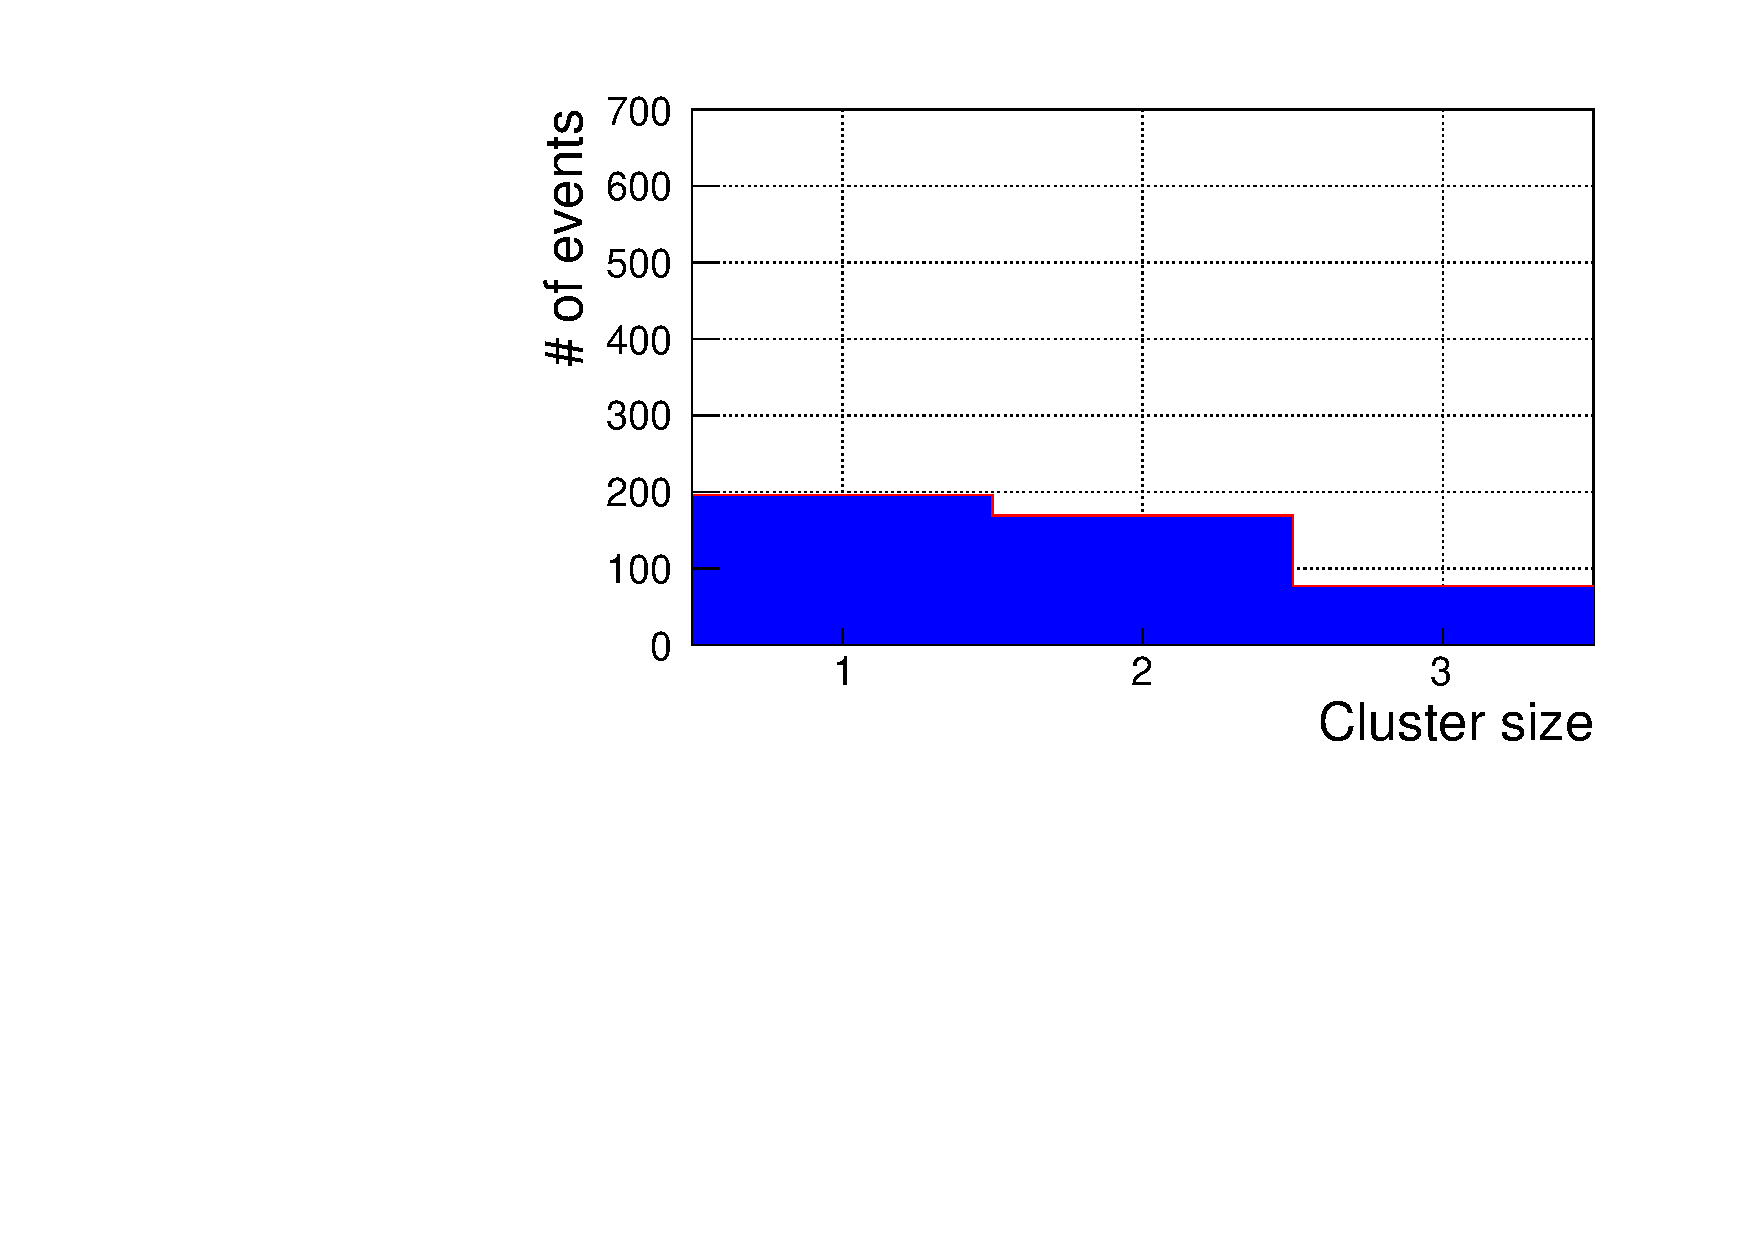
\includegraphics[width=1.1\linewidth]{fig/chapt6/Muon-ClS-1D-5000-gRPC-INFN.pdf}
			\caption{\label{fig:cluster-size-1D:A} \SI{5120}{V}}
		\end{subfigure}
		\begin{subfigure}{.33\linewidth}
		    \centering
			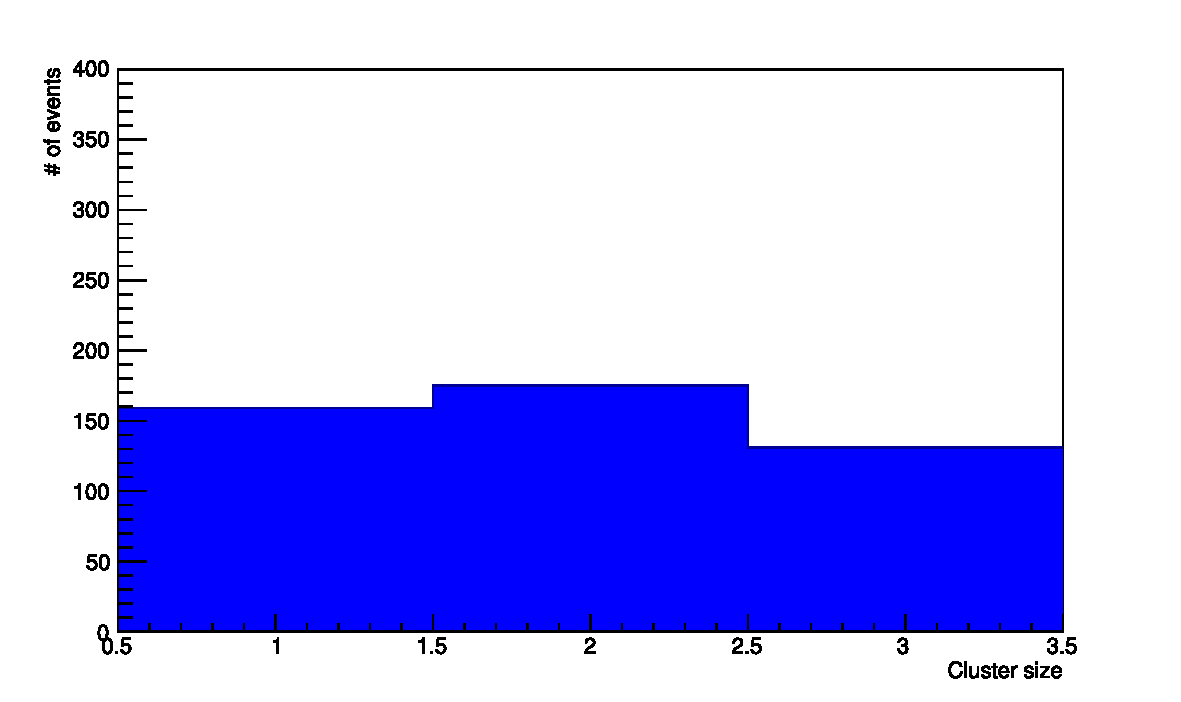
\includegraphics[width=1.1\linewidth]{fig/chapt6/Muon-ClS-1D-5100-gRPC-INFN.pdf}
			\caption{\label{fig:cluster-size-1D:B} \SI{5222}{V}}
		\end{subfigure}
		\begin{subfigure}{.33\linewidth}
		    \centering
			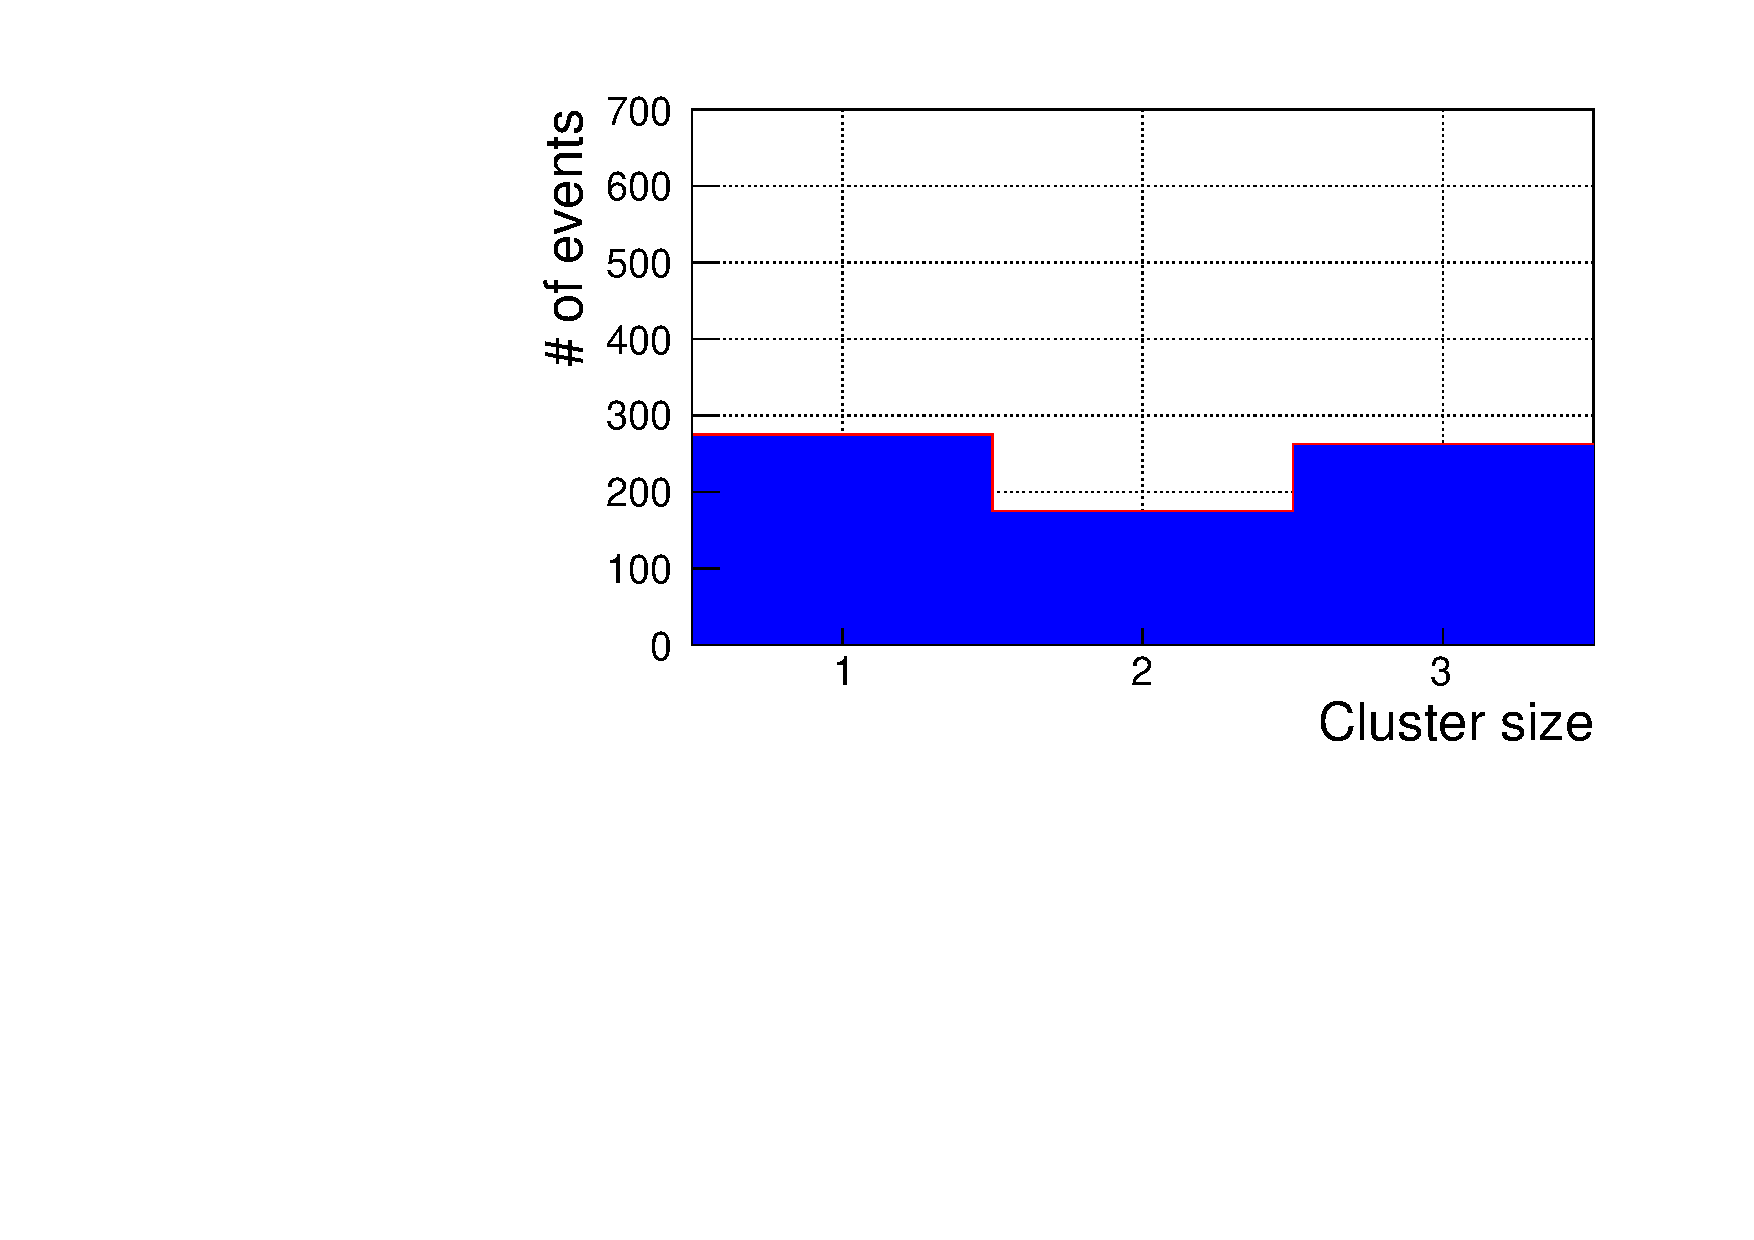
\includegraphics[width=1.1\linewidth]{fig/chapt6/Muon-ClS-1D-5200-gRPC-INFN.pdf}
			\caption{\label{fig:cluster-size-1D:C} \SI{5324}{V}}
		\end{subfigure}
		\begin{subfigure}{.33\linewidth}
		    \centering
			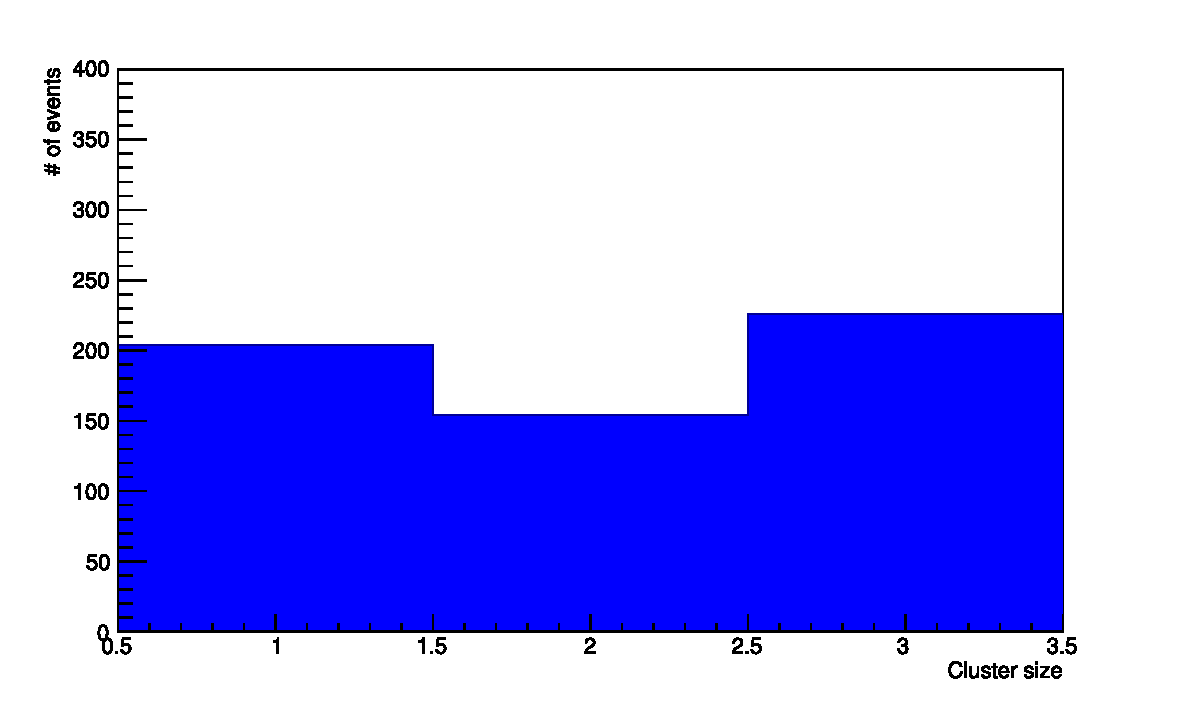
\includegraphics[width=1.1\linewidth]{fig/chapt6/Muon-ClS-1D-5300-gRPC-INFN.pdf}
			\caption{\label{fig:cluster-size-1D:D} \SI{5423}{V}}
		\end{subfigure}
		\begin{subfigure}{.33\linewidth}
		    \centering
			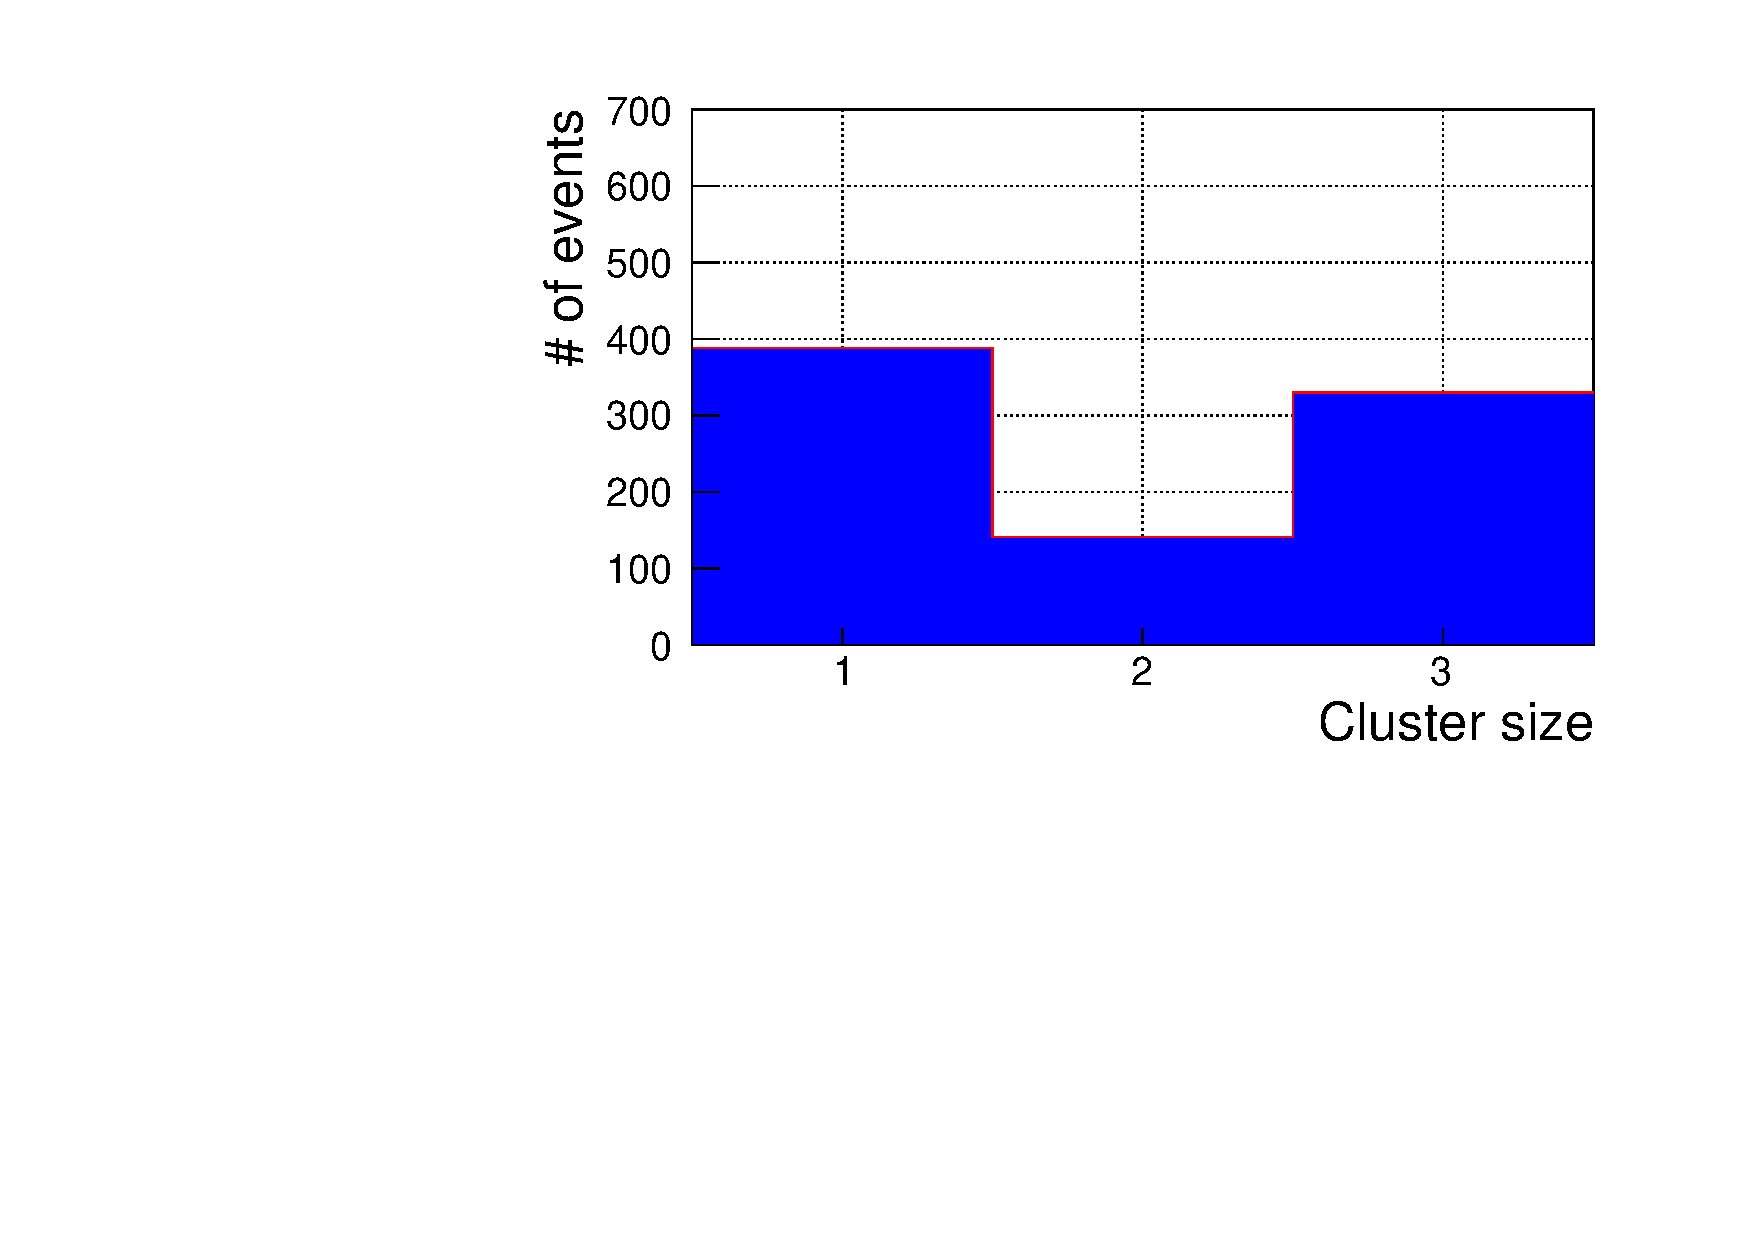
\includegraphics[width=1.1\linewidth]{fig/chapt6/Muon-ClS-1D-5400-gRPC-INFN.pdf}
			\caption{\label{fig:cluster-size-1D:E} \SI{5524}{V}}
		\end{subfigure}
		\begin{subfigure}{.33\linewidth}
		    \centering
			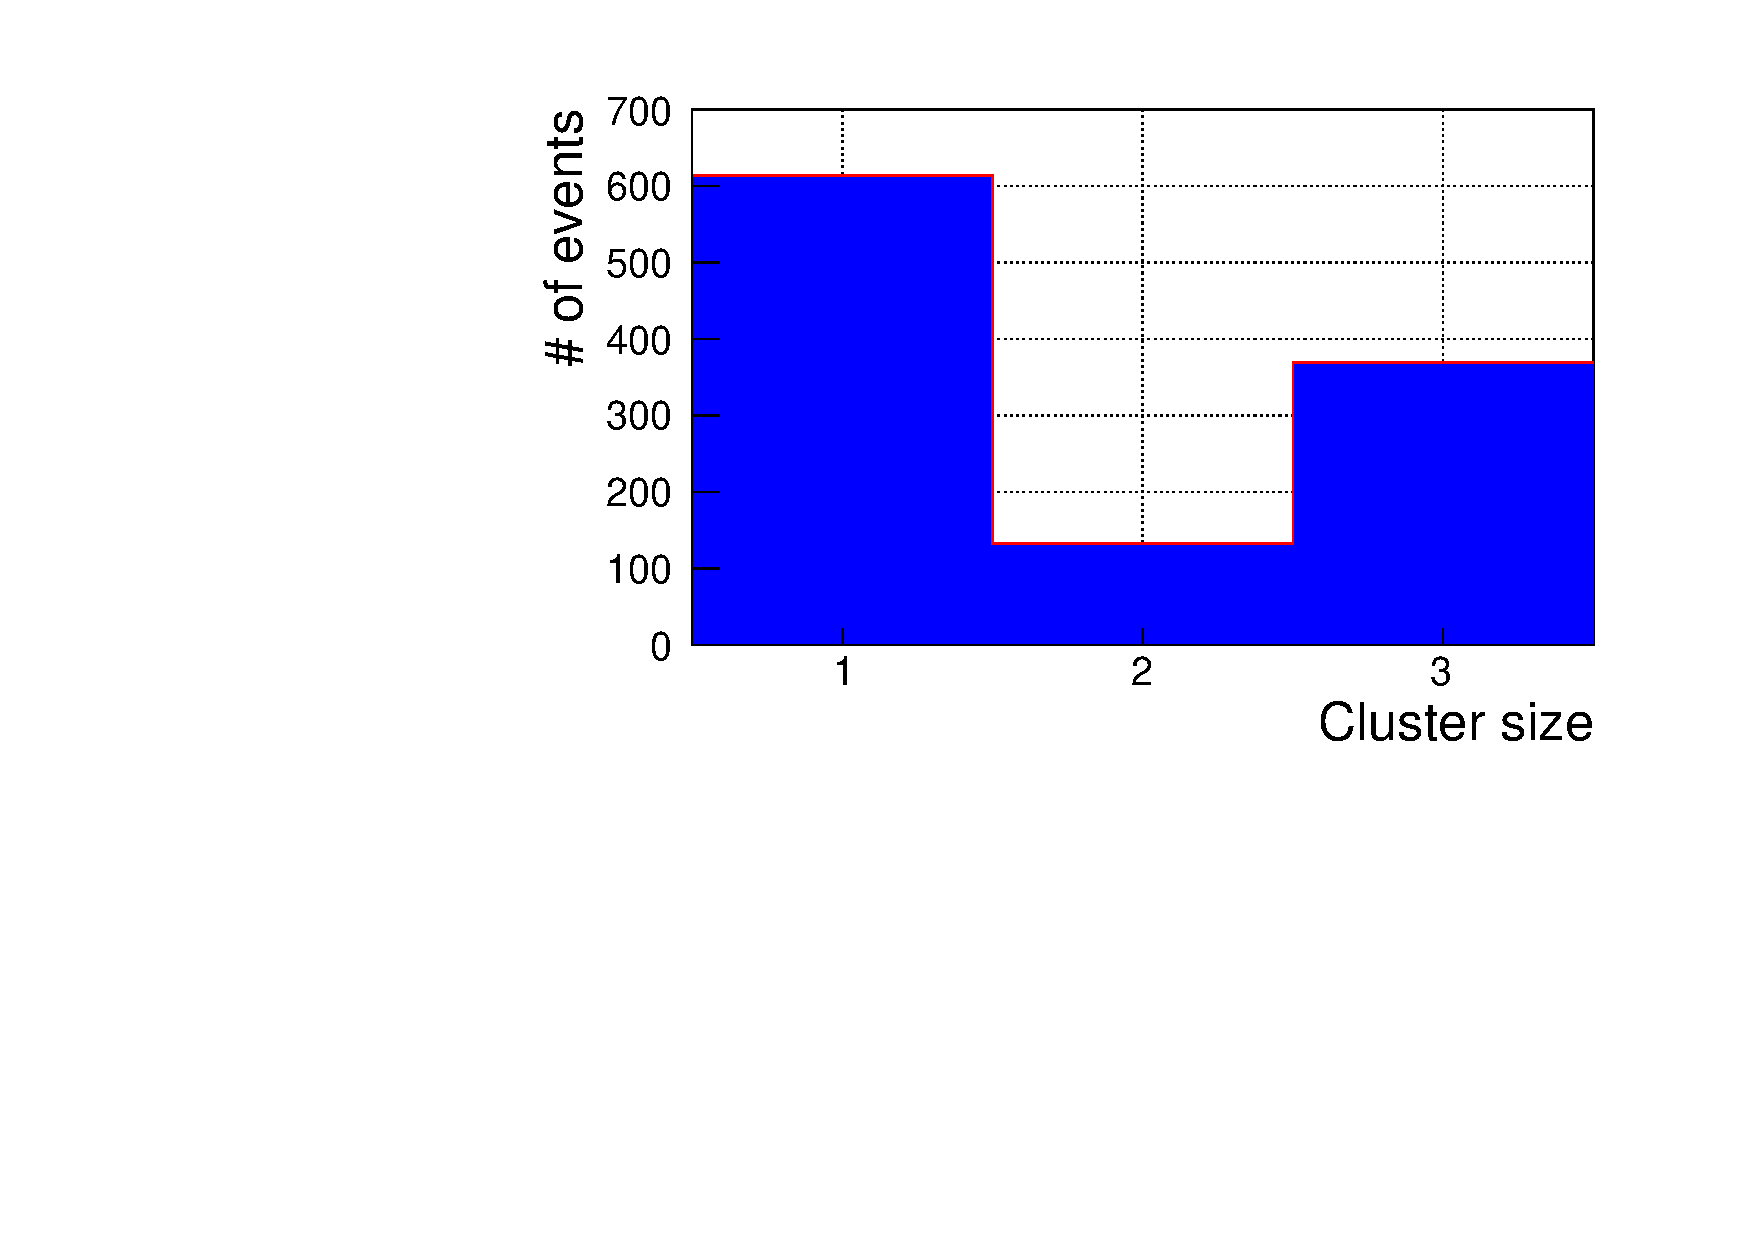
\includegraphics[width=1.1\linewidth]{fig/chapt6/Muon-ClS-1D-5500-gRPC-INFN.pdf}
			\caption{\label{fig:cluster-size-1D:F} \SI{5630}{V}}
		\end{subfigure}
		\caption{\label{fig:cluster-size-1D} Evolution of the cluster size distribution with increasing voltage for the gRPC tested with the INFN preamplifiers using a threshold of \SI{5}{fC}.}
	\end{figure}
	
	\begin{figure}[H]
		\begin{subfigure}{.33\linewidth}
		    \centering
			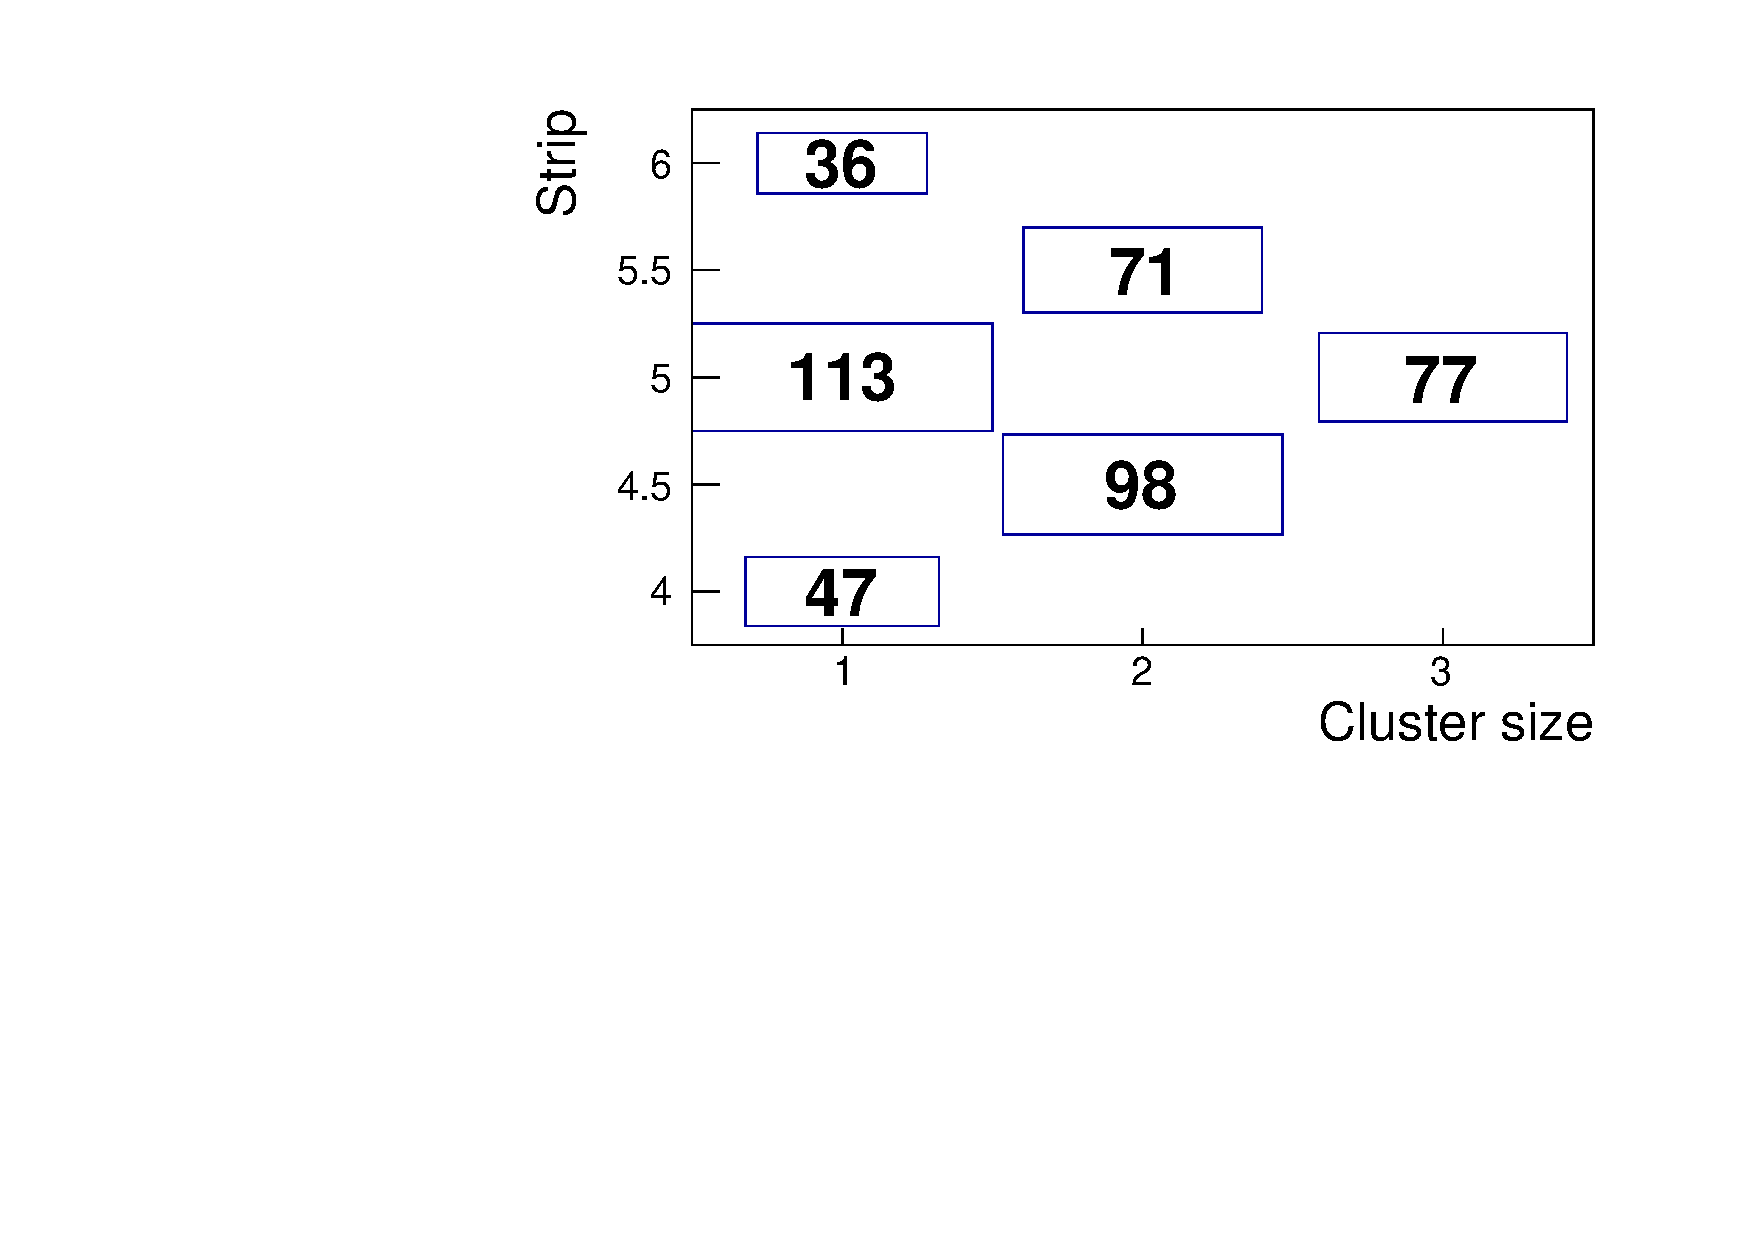
\includegraphics[width=1.1\linewidth]{fig/chapt6/Muon-ClS-5000-gRPC-INFN.pdf}
			\caption{\label{fig:cluster-size-2D:A} \SI{5120}{V}}
		\end{subfigure}
		\begin{subfigure}{.33\linewidth}
		    \centering
			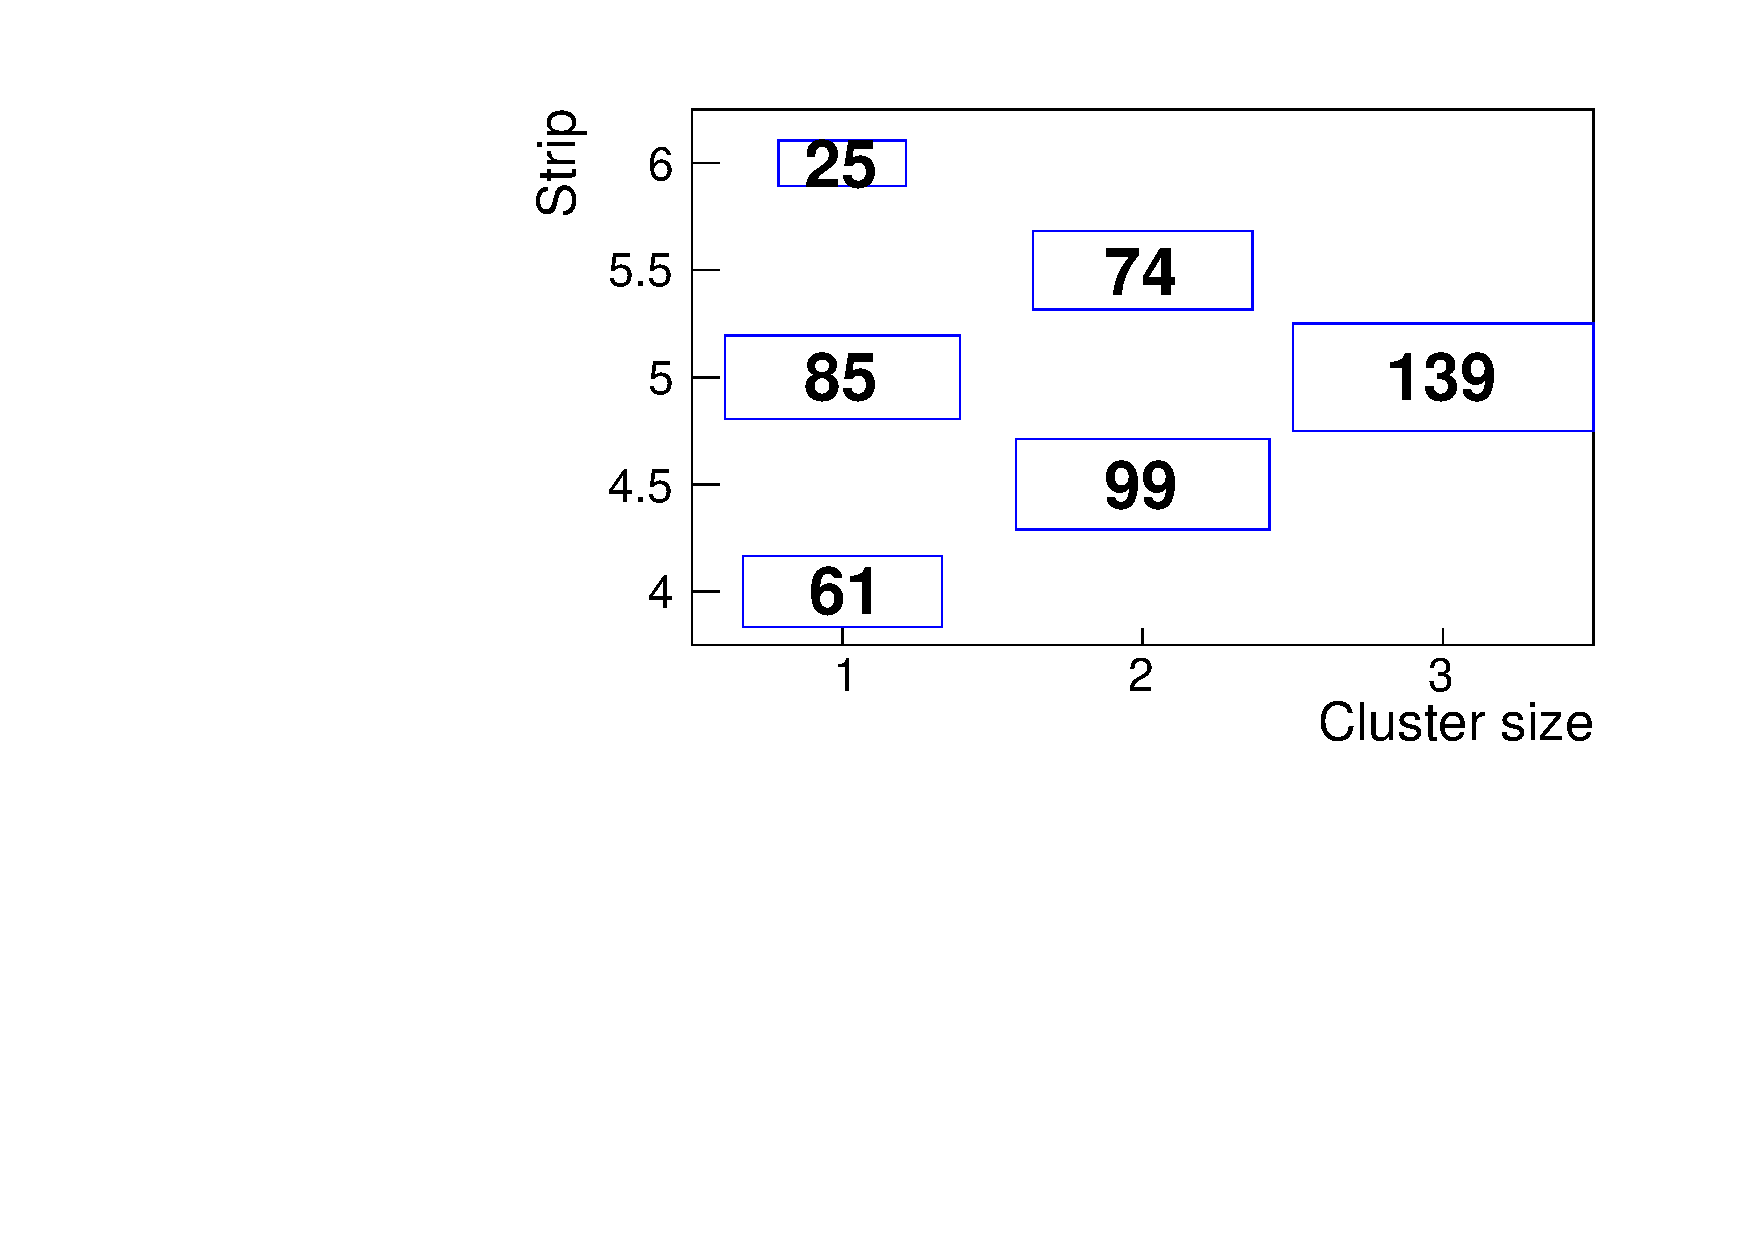
\includegraphics[width=1.1\linewidth]{fig/chapt6/Muon-ClS-5100-gRPC-INFN.pdf}
			\caption{\label{fig:cluster-size-2D:B} \SI{5222}{V}}
		\end{subfigure}
		\begin{subfigure}{.33\linewidth}
		    \centering
			\includegraphics[width=1.1\linewidth]{fig/chapt6/Muon-ClS-5200-gRPC-INFN.pdf}
			\caption{\label{fig:cluster-size-2D:C} \SI{5324}{V}}
		\end{subfigure}
		\begin{subfigure}{.33\linewidth}
		    \centering
			\includegraphics[width=1.1\linewidth]{fig/chapt6/Muon-ClS-5300-gRPC-INFN.pdf}
			\caption{\label{fig:cluster-size-2D:D} \SI{5423}{V}}
		\end{subfigure}
		\begin{subfigure}{.33\linewidth}
		    \centering
			\includegraphics[width=1.1\linewidth]{fig/chapt6/Muon-ClS-5400-gRPC-INFN.pdf}
			\caption{\label{fig:cluster-size-2D:E} \SI{5524}{V}}
		\end{subfigure}
		\begin{subfigure}{.33\linewidth}
		    \centering
			\includegraphics[width=1.1\linewidth]{fig/chapt6/Muon-ClS-5500-gRPC-INFN.pdf}
			\caption{\label{fig:cluster-size-2D:F} \SI{5630}{V}}
		\end{subfigure}
		\caption{\label{fig:cluster-size-2D} Map of the cluster size distribution as a function of the cluster position with increasing voltage for the gRPC tested with the INFN preamplifiers using a threshold of \SI{5}{fC}.}
	\end{figure}
	
\newpage
	
	\begin{figure}[H]
		\begin{subfigure}{.5\linewidth}
		    \centering
			\includegraphics[width=\linewidth]{fig/chapt6/Noise-Profile-gRPC-CMS-FEB.pdf}
			\caption{\label{fig:gRPC-noise:A}}
		\end{subfigure}
		\begin{subfigure}{.5\linewidth}
		    \centering
			\includegraphics[width = \linewidth]{fig/chapt6/Noise-Profile-gRPC-INFN.pdf}
			\caption{\label{fig:gRPC-noise:B}}
		\end{subfigure}
		\caption{\label{fig:gRPC-noise} Noise profile measured in the glass RPC built by Ghent tested with the standard CMS FEB~\subref{fig:gRPC-noise:A} and the INFN preamplifiers mounted on a CMS-like FEB~\subref{fig:gRPC-noise:B}.}
	\end{figure}
    
    \begin{figure}[H]
		\begin{subfigure}{.5\linewidth}
		    \centering
			\includegraphics[width = .8\linewidth]{fig/chapt6/Muon-Time-Profile-gRPC-CMS-FEB.pdf}
			\caption{\label{fig:time-profiles:A}}
		\end{subfigure}
		\begin{subfigure}{.5\linewidth}
		    \centering
			\includegraphics[width = .8\linewidth]{fig/chapt6/Muon-Time-Profile-gRPC-INFN.pdf}
			\caption{\label{fig:time-profiles:B}}
		\end{subfigure}
		\begin{subfigure}{\linewidth}
		    \centering
			\includegraphics[width = .4\linewidth]{fig/chapt6/Muon-Time-Profile-RE2-INFN.pdf}
			\caption{\label{fig:time-profiles:C}}
		\end{subfigure}
		\caption{\label{fig:time-profiles} The arrival time of the hits recorded in the gRPC tested with the CMS FEB~\subref{fig:time-profiles:A} and with the INFN preamplifiers~\subref{fig:time-profiles:B}, and recorded in the CMS RE2 RPC tested with the INFN preamplifiers~\subref{fig:time-profiles:C}.}
	\end{figure}
    
    Even though the performance of the detector are promising, the results concerning the noise rate per unit area seem to indicate that the detector operated with the INFN Tor Vergata electronics produces very high levels of noise, if compared to the noise measured in the RE4 detector. With each type of electronics, the noise doesn't indicate a clear correlation with increasing voltage. The hypothesis at this stage would be that the noise is not created inside of the gas volume by avalanches triggered along the glueing lines, where the electric field could be abruptly perturbated. It would rather come from the read-out channel itself, and from its connection to the electronics. Indeed, looking at the noise profile measured in the detector and presented in Figure~\ref{fig:gRPC-noise:A}, it is clear that the noise is localised in two areas corresponding to the HV connectors in the case of the HV scan performed with the CMS FEB. Moreover, contrary to the very careful work performed on the RE2 chamber to match the impedance of the strips with the read-out cables connected to the board on which the INFN preamplifiers are mounted, no matching was done on the gRPC due to a lack of time. The noise measured in the tested three channels is shown in Figure~\ref{fig:gRPC-noise:B}. This region of the detector doesn't correspond to the HV connectors according to Figure~\ref{fig:gRPC-noise:A}. Nevertheless, the number of hits counted in the detector is much higher than in the CMS FEB case. Looking more carefully to Figure~\ref{fig:time-profiles} presenting the hit time profile in both cases together with the time profile of the CMS RE2-2 detector tested with INFN preamplifiers, it is clear that the detector is noisier. Also, the reflections due to the impedance mismatch is clearly visible in Figure~\ref{fig:time-profiles:B}.

	\subsection{HARDROC 2 based RPC read-out}
	\label{chapt6:ssec:HARDROC2}
	
	The \acf{HARDROC} ASIC, as its name suggests, has been developed for RPC applications and in particular for the read-out RPCs of the SDHCAL that is being studied in the perspective of the ILC. The SDHCAL detectors are required to have a high granularity compared to the CMS RPCs and hence, they use \SI{1}{cm^2} read-out pads instead of strips. This choice results in a huge number of channels. The ASIC is mounted directly on the read-out pannel for compactness as can be seen in Figure~\ref{fig:Setup-HARDROC2:A} and feature three thresholds to provide a semi-digital information.
	 
	\begin{figure}[H]
		\begin{subfigure}{.5\linewidth}
		    \centering
			\includegraphics[width = \linewidth]{fig/chapt6/Setup_HARDROC_PAK.jpg}
			\caption{\label{fig:Setup-HARDROC2:A}}
		\end{subfigure}
		\begin{subfigure}{.5\linewidth}
		    \centering
			\includegraphics[width = \linewidth]{fig/chapt6/Setup_HARDROC_gRPC.JPG}
			\caption{\label{fig:Setup-HARDROC2:B}}
		\end{subfigure}
		\caption{\label{fig:Setup-HARDROC2} Experimental setups used to test the HARDROC2 electronics with a CMS RE4-3 gap~\subref{fig:Setup-HARDROC2:A} and a gRPC gap built in Ghent~\subref{fig:Setup-HARDROC2:B}.}
    \end{figure}
	
	The PETIROC uses a similar technology than the one developed for the HARDROC and is manufactured by the same company. It is safe to conclude that the preliminary results obtained with the HARDROC electronics constitute a strong indication on the potential performance of a FEB developed specifically for CMS detectors. The leading institute in the development of the SDHCAL based on single-gap \acf{gRPCs} is the IPNL which also played a great role in developing iRPCs for CMS.
	
\begingroup\setlength{\intextsep}{5pt}\setlength{\columnsep}{15pt}

	\begin{wrapfigure}{O}{.4\linewidth}
	    \centering
		\includegraphics[width = \linewidth]{fig/chapt6/HARDROC_chip.JPG}
		\caption{\label{fig:HARDROC2-chip} HARDROC2 control chip with its "Mezzanine" used to collect the data from the different HARDROC ASICs and communicate with the computer. On top of the picture, the trigger is brought by a coaxial cable. The connection with the computer is assured by both the USB cables.}
    \end{wrapfigure}
	
	A read-out pannel using the HARDROC 2 technology was lent by this institute and was tested onto a CMS RPC. Contrary to the tests with the INFN preamplifiers that were made using an RE2-2 CMS RPC built in 2007 for the second endcap disk of CMS, the choice was made to use an RE4-3 detector built during LS1 to equip the fourth endcap. Indeed, the pannel can't be sandwiched between two RPC gaps due to the embedded electronics and a single CMS RPC gap was used. At the time of this experiment, only spare RE4-3 gaps were available. The choice was then made to change detector with respect to the previous series of tests conducted on the INFN preamplifiers. As for the INFN preamplifiers, the pannel has been tested on the gRPC built by UGent. The gRPC being smaller than the HARDROC read-out that was used for the experiment but thanks to the 2D read-out using pads, this was not a problem for the data acquisition.
	
	Once again, the experiment was conducted in the CMS RPC assembly laboratory at CERN. The two different setups are shown in Figure~\ref{fig:Setup-HARDROC2}. The read-out panel is placed directly on top of the gaps and pressed against the detector surface thanks to weights. The same PMT telescope is used to provide a trigger to the data acquisition. In the particular case of the HARDROC 2 electronics, the output signal does not correspond to the LVDS signals provided by the CMS FEB. Moreover, there would be more than 1500 channels to constantly monitor and unfortunately, there would not be enough VME TDC modules to use with the DAQ software designed for the experiment involving the INFN preamplifiers. Nevertheless, a custom-made DAQ software was designed by the members of IPNL's team to read-out the electronics through the chip presented in Figure~\ref{fig:HARDROC2-chip}. The data are continuously stored in the buffer of the ASIC and dumped into the computer when a trigger signal is received.
	
\endgroup
	
	The results of the tests conducted with the HARDROC 2 on a CMS gap are presented in Figure~\ref{fig:HARDROC2} and Table~\ref{tab:HARDROC2}. These results can hardly be compared to what was measured with the INFN preamplifiers as the detector was not tested using the single-gap mode. The tested thresholds are high compared to the ones displayed by the INFN preamplifiers and are of the order of magnitude of the current CMS FEB. Nevertheless, the performance of the detector equipped with this read-out pannel is measured to be better. Indeed, a shift of 400 to \SI{500}{V} is observed at thresholds ranging from 230 to \SI{121.4}{fC}. This could be explained by the difference in read-out channel areas of both read-out panels. Indeed, in the case of the standard CMS RPC, the read-out panel consists in relatively large trapezoidal strips with a surface of almost \SI{200}{cm^2} when the read-out of the HARDROC 2 is composed of \SI{1}{cm^2} pads. Also taking into account the cross-talk between adjacent channels, the charge produced by a growing avalanche is spread over a larger surface in the case of the standard CMS RPC. Finally, the signals having to travel a longer distance to reach the electronics, the signal loss leads to a smaller signal relative to the pads.\\
	The cluster size is provided for information as a direct comparison of the cluster size measured with \SI{1}{cm^2} pads and long copper strips with width of a few \si{cm} is not possible. The measured cluster size at working voltage with the CMS FEB is consistent with what would be expected of a single-gap RPC. Indeed, the usage of two gaps in an OR system allows for a stronger overall gain and hence, the cluster size is greater. A more precise estimation of the charge spread inside of the gap is obtained using pads instead of strips. At working voltage, an avalanche is detected within less than two pads on average. An extra information could be used to further improve the spatial resolution of the detector. Indeed, the HARDROC 2 are semi-digital electronics and feature three threshold levels. Tuning these thresholds would lead to an approximation of the induced charge profile over the neighbouring pads. A gaussian fit over the digitized distribution would give an estimation of the position of the avalanche center.
	
	\begin{figure}[H]
		\begin{subfigure}{.5\linewidth}
		    \centering
			\includegraphics[width=\linewidth]{fig/chapt6/HARDROC2-Eff-Shift.pdf}
			\caption{\label{fig:HARDROC2:A}}
		\end{subfigure}
		\begin{subfigure}{.5\linewidth}
		    \centering
			\includegraphics[width = \linewidth]{fig/chapt6/HARDROC2-ClS-Shift.pdf}
			\caption{\label{fig:HARDROC2:B}}
		\end{subfigure}
		\begin{subfigure}{\linewidth}
		    \centering
			\includegraphics[width = .5\linewidth]{fig/chapt6/HARDROC2-Rate-Shift.pdf}
			\caption{\label{fig:HARDROC2:C}}
		\end{subfigure}
		\caption{\label{fig:HARDROC2} Efficiency~\subref{fig:HARDROC2:A}, cluster size~\subref{fig:HARDROC2:B} and noise rate per unit area~\ref{fig:HARDROC2:C} of the CMS RE4-3 detector tested in single gap mode with the standard CMS FEBs (black) and with the HARDROC 2 readout panel at different thresholds (red, blue and pink).}
	\end{figure}
	
\newpage
	
	\begin{table}[H]
		\caption{\label{tab:HARDROC2} Results of the sigmoid fit (Formula~\ref{eq:Sigmoid}) performed on the data presented in Figure~\ref{fig:HARDROC2:A}. The working point and its corresponding efficiency are computed using Formulas~\ref{eq:Sigmoid} and \ref{eq:KneeWP}.}
		\footnotesize
		\begin{tabular}{|c|c|c|c|c|c|}
			\hline
			Data & $\epsilon_{max}$ & $\lambda$ ($\cdot$\Ord{-2} \si{V^{-1}}) & $HV_{50}$ (\si{V}) & $\epsilon_{WP}$ & $HV_{WP}$ (\si{V}) \\ 
			\hline
			CMS FEB, 143fC (2014) & $0.958 \pm 0.000$ & $0.75 \pm 0.00$ & $9174 \pm 1$ & $0.94 \pm 0.00$ & $9716 \pm 2$\\ 
			\hline
			HARDROC 2, 230fC (2015) & $0.987 \pm 0.002$ & $1.06 \pm 0.04$ & $8905 \pm 8$ & $0.98 \pm 0.01$ & $9333 \pm 17$\\ 
			\hline
			HARDROC 2, 143fC (2015) & $0.988 \pm 0.001$ & $1.10 \pm 0.04$ & $8826 \pm 8$ & $0.98 \pm 0.01$ & $9243 \pm 17$\\ 
			\hline
			HARDROC 2, 121.4fC (2015) & $0.987 \pm 0.001$ & $1.07 \pm 0.04$ & $8795 \pm 8$ & $0.98 \pm 0.01$ & $9220 \pm 17$\\ 
			\hline
		\end{tabular}
	\end{table}
	
	Finally, the noise measured in the electronics is of the same order of what had been measured in Figure~\ref{fig:INFN-FEB:C}. It is safe to assume that the noise level in the case of a single-gap RPC is expected to be of the same order of magnitude than its double-gap counterpart as the noise mainly is electromagnetic. Figure~\ref{fig:HARDROC2-profiles} provides a clearer understanding of the position of the trigger PMTs and of the noise measured with the HARDROC. The noise of the electronics itself is very small, and the read-out pannel is sensitive enough to measure the noise in the RPC gap. Indeed, except for a few visible hot spots, the observed noise profile corresponds perfectly to the spacer positions inside of the gap volume. The PET buttons used to maintain the uniformity of the gas volume cause noise at their proximity as they modify the local electric field.
	 
	\begin{figure}[H]
		\begin{subfigure}{.5\linewidth}
		    \centering
			\includegraphics[width = \linewidth]{fig/chapt6/Muon-Profile-RE4-HARDROC.pdf}
			\caption{\label{fig:HARDROC2-profiles:A}}
		\end{subfigure}
		\begin{subfigure}{.5\linewidth}
		    \centering
			\includegraphics[width = \linewidth]{fig/chapt6/Noise-Profile-RE4-HARDROC.pdf}
			\caption{\label{fig:HARDROC2-profiles:B}}
		\end{subfigure}
		\caption{\label{fig:HARDROC2-profiles} Measured muon~\subref{fig:HARDROC2-profiles:A} and noise~\subref{fig:HARDROC2-profiles:B} profiles in the read-out pads of the HARDROC 2 over a CMS RE4-3 gap. The inner structure of the gap and the presence of the spacers in the volume is visible.}
    \end{figure}
	
	The results of the experiment with the gRPC are provided in Figure~\ref{fig:HARDROC2-gRPC} and Table~\ref{tab:HARDROC2-gRPC}. Unfortunately the gRPC had not been tested in single gap mode with the CMS FEB. Thus, a direct comparison is not possible as the data were not collected in similar conditions. The detector could only be tested with a single HARDROC 2 threshold setting (\SI{143}{fC}). As for the double-gap, the efficiency of the single-gap reaches 95\% at working voltage. The working voltage is consistent with the double-gap detector operated with the CMS FEB indicating that the HARDROC is more sensitive to lower charges. The difference in efficiency rising is consistent with the use of one gap versus two in the case of the CMS FEB. The working voltage in the case of the HARDROC 2 in single gap mode is comparable to the one obtained with the standard CMS FEB in double gap mode even though both electronics were operated at the same detection threshold. This confirms that the HARDROC 2 is more sensitive than the CMS FEB in the same conditions. Again, the explanation could be found in the different read-out panels. When operated with the CMS FEB, the gRPC is read out by copper strips with a surface of \SI{45}{cm^2} to be compared with the \SI{1}{cm^2} of the HARDROC 2 read-out.\\
	As discussed in the case of the CMS RE4-3 gap, the direct comparison of the cluster sizes is not possible. In this sense, the proximity of both results only is fortuitous. The cluster size of approximately 1.6 measured with the HARDROC 2 at working voltage is of the same order than what had previously been measured for the CMS gap indicating that at equivalent performance, the gain and hence, the induced charge could be comparable.
	
	\begin{figure}[H]
		\begin{subfigure}{.5\linewidth}
		    \centering
			\includegraphics[width=\linewidth]{fig/chapt6/gRPC-HARDROC2-Eff-Shift.pdf}
			\caption{\label{fig:HARDROC2-gRPC:A}}
		\end{subfigure}
		\begin{subfigure}{.5\linewidth}
		    \centering
			\includegraphics[width = \linewidth]{fig/chapt6/gRPC-HARDROC2-ClS-Shift.pdf}
			\caption{\label{fig:HARDROC2-gRPC:B}}
		\end{subfigure}
		\begin{subfigure}{\linewidth}
		    \centering
			\includegraphics[width = .5\linewidth]{fig/chapt6/gRPC-HARDROC2-Rate-Shift.pdf}
			\caption{\label{fig:HARDROC2-gRPC:C}}
		\end{subfigure}
		\caption{\label{fig:HARDROC2-gRPC} Efficiency~\subref{fig:HARDROC2:A}, cluster size~\subref{fig:HARDROC2:B} and noise rate per unit area~\subref{fig:HARDROC2:C} of the UGent gRPC tested in double-gap mode with the standard CMS FEBs (black) and in single-gap with the HARDROC 2 readout panel at a threshold of \SI{143}{fC} (red).}
	\end{figure}
	
	\begin{table}[H]
		\caption{\label{tab:HARDROC2-gRPC} Results of the sigmoid fit (Formula~\ref{eq:Sigmoid}) performed on the data presented in Figure~\ref{fig:HARDROC2-gRPC:A}. The working point and its corresponding efficiency are computed using Formulas~\ref{eq:Sigmoid} and \ref{eq:KneeWP}.}
		\footnotesize
		\begin{tabular}{|c|c|c|c|c|c|}
\hline
Data & $\epsilon_{max}$ & $\lambda$ ($\cdot$\Ord{-2} \si{V^{-1}}) & $HV_{50}$ (\si{V}) & $\epsilon_{WP}$ & $HV_{WP}$ (\si{V}) \\ 
\hline
CMS FEB, 143fC (2015)   & $0.956 \pm 0.007$ & $0.86 \pm 0.04$ & $5349 \pm 8$ & $0.94 \pm 0.01$ & $5839 \pm 23$\\ 
\hline
HARDROC 2, 143fC (2015) & $0.966 \pm 0.004$ & $0.64 \pm 0.02$ & $5179 \pm 7$ & $0.95 \pm 0.01$ & $5790 \pm 25$\\ 
\hline
		\end{tabular}
	\end{table}
	
	Finally, the noise measured in the electronics seemed higher than in the case of the CMS gap. Looking closer to the noise profile provided in Figure~\ref{fig:HARDROC2-gRPC-profiles}, it can be seen that the noise measurement was affected by the HV connector. Indeed, the high noise measured in pads 41 and 42 along X and 22 to 25 along Y, corresponds exactly to the position of the HV connector on the cathode side. Contrary to the case of the CMS gap where the HV connector was far from the read-out area, the gRPC is smaller than the read-out and due to the poor grounding of the setup the electric field created by the HV connector could affect the read-out. Excluding the corresponding pads gives a much more reliable noise measurement as can be seen in Figure~\ref{fig:HARDROC2-gRPC:C}. A better understanding of the gRPC uniformity can be obtained through the noise profile. First of all, the row corresponding to Y=16 seems consistently noisier than the neighbouring pads an could correspond to the glueing line that lies along this pad row. Nonetheless, the increase of the noise along this line is not very clear, and no corresponding behaviour can be observed along the other glueing line along column X=30. But the gas volume corresponding to the largest glass plate, spreading from columns 31 to 47 along X and rows 1 to 15 clearly shows a stronger noise in its center. The detection area being small, only a few ceramic ball spacers were used to maintain the distance in between the electrodes. It not impossible that the ball spacer located in the center of this very volume popped out. Due to the absence of a spacer, the force applied by electric field onto the electrodes could have made the distance in between the electrodes smaller and artificially increased the observed electric field, also increasing the measured noise.
	 
	\begin{figure}[H]
		\begin{subfigure}{.5\linewidth}
		    \centering
			\includegraphics[width = \linewidth]{fig/chapt6/Muon-Profile-gRPC-HARDROC.pdf}
			\caption{\label{fig:HARDROC2-gRPC-profiles:A}}
		\end{subfigure}
		\begin{subfigure}{.5\linewidth}
		    \centering
			\includegraphics[width = \linewidth]{fig/chapt6/Noise-Profile-gRPC-HARDROC.pdf}
			\caption{\label{fig:HARDROC2-gRPC-profiles:B}}
		\end{subfigure}
		\caption{\label{fig:HARDROC2-gRPC-profiles} Measured muon~\subref{fig:HARDROC2-gRPC-profiles:A} and noise~\subref{fig:HARDROC2-gRPC-profiles:B} profiles in the read-out pads of the HARDROC 2 over a gRPC gap built by Ghent.}
    \end{figure}
    
	\section{Outlook on the current FEE certification status}
	\label{chapt6:sec:outlooks}
	
	In this Section the ongoing certification of the PETIROC FEB and of the INFN Tor Vergata FEBs, chosen as back-up solution, will be presented. For reference, an iRPC has been operated without irradiation with the standard CMS FEB. It is reminded that the iRPCs that will complete the redundancy of the muon system of CMS close to the beam line are expected to suffer a background hit rate per unit area of \SIrate{600}. Including a safety factor of 3, it is then necessary for the detectors to be certified at a minimal background hit rate of \SIkrate{2}.
	
		\subsection{CMS \acl{FEB} reference}
		\label{chapt6:ssec:CMSFEBref}
    
    The iRPCs that will be installed at CMS will be equipped with new \acl{FEE}. Nevertheless, in order to compare the performance of the new electronics with the standard CMS FEBs, a series of short characterization tests was carried out with an iRPC prototype. Seven strips of a read-out panel designed for a back-up scenario detector were connected to a CMS FEB. The remaining strips were connected to the ground to avoid noise. The tests were done without irradiation and using cosmic muons. Two narrow scintillators were placed on each side of the prototype to provide a trigger signal as can be seen from Figure~\ref{fig:iRPC_CMS_Setup}. The tests were performed with three detection thresholds of \SI{200}{mV} ($\approx$\SI{133}{fC}), \SI{210}{mV} ($\approx$\SI{140}{fC}) and \SI{220}{mV} ($\approx$\SI{146}{fC}) on the FEB discriminators. The LVDS output of the FEB was then read-out with a CAEN TDC.\\
    The HV scans consisted of seven effective voltage steps (6800, 7000, 7100, 7200, 7300, 7400 and \SI{7500}{V}) at which 100 muon triggers were requested as minimal statistics. The hit profile over the connected strips as well as the time profile of the events in each channel is provided in Figure~\ref{fig:iRPC_CMS_Profiles} for the fifth HV step (\SI{7300}{HV}). The area covered by the trigger is seen to be comparable than the width of the seven strips. The time arrival of the hits is well confined within less than \SI{50}{ns}.
		
	\begin{figure}[H]
		\centering
		\includegraphics[width = 0.7\linewidth]{fig/chapt6/iRPC-CMS_FEB-Setup.png}
		\caption{\label{fig:iRPC_CMS_Setup} Experimental setup used to test the iRPC equipped with the standard CMS FEEs. Seven of the 96 strips are connected to the read-out channels.}
    \end{figure}

	\begin{figure}[H]
		\begin{subfigure}{0.5\linewidth}
		    \centering
			\includegraphics[width = .8\linewidth]{fig/chapt6/iRPC-CMS_FEB-HitProfile.png}
			\caption{\label{fig:iRPC_CMS_Profiles:A}}
		\end{subfigure}
		\begin{subfigure}{0.5\linewidth}
		    \centering
			\includegraphics[width = .8\linewidth]{fig/chapt6/iRPC-CMS_FEB-TimeProfile.png}
			\caption{\label{fig:iRPC_CMS_Profiles:B}}
		\end{subfigure}
		\caption{\label{fig:iRPC_CMS_Profiles} \subref{fig:iRPC_CMS_Profiles:A} Distribution of the muon hits on the seven strips connected to the standard CMS FEB. Strip 8 is connected to the ground. \subref{fig:iRPC_CMS_Profiles:B} Time distribution of the hits in the seven channels. The color scale corresponds to the number of hits per bin.}
    \end{figure}
	 
	\begin{figure}[H]
		\begin{subfigure}{.5\linewidth}
		    \centering
			\includegraphics[width = .9\linewidth]{fig/chapt6/iRPC-CMS_FEB-muonEfficiency.pdf}
			\caption{\label{fig:iRPC_CMS_Result:A}}
		\end{subfigure}
		\begin{subfigure}{.5\linewidth}
		    \centering
			\includegraphics[width = .9\linewidth]{fig/chapt6/iRPC-CMS_FEB-thrs_CLS.pdf}
			\caption{\label{fig:iRPC_CMS_Result:B}}
		\end{subfigure}
		\begin{subfigure}{.5\linewidth}
		    \centering
			\includegraphics[width = .9\linewidth]{fig/chapt6/iRPC-CMS_FEB-thrs_CMP.pdf}
			\caption{\label{fig:iRPC_CMS_Result:C}}
		\end{subfigure}
		\begin{subfigure}{.5\linewidth}
		    \centering
			\includegraphics[width = .9\linewidth]{fig/chapt6/iRPC-CMS_FEB-thrs_noiseRate.pdf}
			\caption{\label{fig:iRPC_CMS_Result:D}}
		\end{subfigure}
		\caption{\label{fig:iRPC_CMS_Result} Summary of the HV scans performed on the iRPC prototype equipped with a standard CMS FEB at three detection thresholds. \subref{fig:iRPC_CMS_Result:A} Efficiency sigmoids. \subref{fig:iRPC_CMS_Result:B} Mean muon cluster size at working voltage. \subref{fig:iRPC_CMS_Result:C} Mean muon cluster multiplicity at working voltage. \subref{fig:iRPC_CMS_Result:D} Noise hit rate per unit area at working voltage.}
    \end{figure}
    
    \begin{table}[H]
		\caption{\label{tab:iRPC-FEB} Summary results of the iRPC operated with a standard CMS RPC FEB.}
		\footnotesize
		\centering
		\begin{tabular}{|c|c|c|c|c|c|}
\hline
Threshold (\si{fC}) & Working Voltage (\si{V}) & Efficiency (\%) & Cluster Size    & Multiplicity    & Noise (\sirate)\\ 
\hline
146                 & $7552 \pm 57$            & $96.6 \pm 1.8$  & $2.34 \pm 0.11$ & $1.02 \pm 0.03$ & $0.21$         \\ 
\hline
140                 & $7473 \pm 49$            & $97.0 \pm 2.5$  & $2.52 \pm 0.18$ & $0.99 \pm 0.07$ & $0.38$         \\ 
\hline
133                 & $7393 \pm 45$            & $96.9 \pm 3.0$  & $2.34 \pm 0.15$ & $0.97 \pm 0.07$ & $0.30$         \\ 
\hline
		\end{tabular}
	\end{table}
    
    The results for this kind of electronics are to be found in Figure~\ref{fig:iRPC_CMS_Result}. First of all, the efficiency at working voltage of the detector reaches 96.9\% at a threshold of \SI{146}{fC}, 97.0\% at \SI{140}{fC} and finally 96.6\% at \SI{133}{fC}. The efficiency does not seem to be affected by a change of threshold. The working voltage, on the other hand, is shifted towards lower effective voltage values with decreasing threshold. The values of working voltages respectively are 7552, 7473 and \SI{7393}{V}. This is expected by the lower gain necessary to produce large enough avalanches. No other differences can be observed at the level of the mean muon cluster sizes, mean muon cluster multiplicity per event and noise rate per unit area. The mean muon cluster size stays of the order of 2.4 strips per cluster and the muon cluster multiplicity, which is the number of reconstructed muon clusters per event, is consistent with 1 as expected. Finally, the noise rate per unit area is below \SIrate{1}. The results are summarized in Table~\ref{tab:iRPC-FEB}.
	
		\subsection{PETIROC FEE}
		\label{chapt6:ssec:RPCROCcert}

\begingroup\setlength{\intextsep}{0pt}\setlength{\columnsep}{15pt}
	
	\begin{wrapfigure}{O}{0.6\linewidth}
		\centering
		\includegraphics[width = 0.9\linewidth]{fig/chapt6/iRPC-RPCROC-H2.png}
		\caption{\label{fig:RPCROCv0_H2} Experimental setup used along the H2 muon beam at CERN to measure the linearity between beam position along the strip length and the time difference measured between both strip ends with the version 0 of the PETIROC FEB.}
    \end{wrapfigure}
		
	Several iRPCs equipped with different versions of PETIROC FEBs have been assembled and tested. This process helped identifying the weaknesses of the FEEs and propose new improved versions. The last piece of the R\&D process will be the FEBv2 equipped with three PETIROC 2C ASICs, three Cyclone V FPGAs hosting the TDCs, and a fourth FPGA to communicate with the back-end electronics.\\
	In a first series of tests performed along the muon beam line H2 at CERN, the FEBv0 was certified for time resolution performances and linearity between the time difference of recorded muon signals measured at both strip ends and the beam position along the strip length. The experimental setup is shown in Figure~\ref{fig:RPCROCv0_H2} on which two iRPCs are placed between two narrow scintillators for a precise knowledge of the position of the beam.\\
	The mean time difference between the signals measured at the high-radius (HR) and low-radius (LR) is given in Figure~\ref{fig:RPCROCv0_Res:A}. The time resolution of the measurement is of \SIerror{252}{4}{ps}. The velocity of propagation $v$ of the signals along the strips was reported to be of \SI{1}{m} per \SI{5.25}{ns}. According to Equation~\ref{eq:Y-determ}, in which $L$ is the length of the strip, $Y$ the position along the strip, and $T_{HR}$ and $T_{LR}$ the measured arrival time at the high-radius and low-radius ends of the strip, the spatial resolution $\Delta Y$ along the strip is then of the order of \SI{2}{cm}. The linearity between the time difference and the position of a hit along the strip length could then be studied with a good precision as can be seen in Figure~\ref{fig:RPCROCv0_Res:B}.
	
\endgroup
	
    \begin{equation}
		\label{eq:Y-determ}
		\begin{aligned}
			Y &= \frac{L}{2} - \frac{v}{2} \times (T_{HR}-T_{LR})\\
			\Delta Y &= \frac{v}{2} \times \Delta(T_{HR}-T_{LR})
		\end{aligned}
    \end{equation}
    
\newpage
	 
	\begin{figure}[H]
		\begin{subfigure}{.5\linewidth}
		    \centering
			\includegraphics[width = \linewidth]{fig/chapt6/iRPC-RPCROC-TimeResolution.png}
			\caption{\label{fig:RPCROCv0_Res:A}}
		\end{subfigure}
		\begin{subfigure}{.5\linewidth}
		    \centering
			\includegraphics[width = \linewidth]{fig/chapt6/iRPC-RPCROC-Linearity.png}
			\caption{\label{fig:RPCROCv0_Res:B}}
		\end{subfigure}
		\caption{\label{fig:RPCROCv0_Res} \subref{fig:RPCROCv0_Res:A} Average time resolution of the iRPC equipped with the FEBv0. \subref{fig:RPCROCv0_Res:B} Linearity between reconstructed beam position along the strip length and the time difference measured between both strip ends.}
    \end{figure}

\begingroup\setlength{\intextsep}{5pt}\setlength{\columnsep}{15pt}
	
	\begin{wrapfigure}{O}{0.6\linewidth}
		\centering
		\includegraphics[width = 0.9\linewidth]{fig/chapt6/iRPC-RPCROC-GIFpp.png}
		\caption{\label{fig:RPCROCv1_GIFpp} Experimental setup used at the GIF++ to certify the iRPC equipped with the version 1 of the PETIROC FEB. The chamber is placed along the beam line in front the Cesium source.}
    \end{wrapfigure}
    
    Later on, a new iRPC was assembled with FEBv1 using first PETIROC 2A. This version is referred to as FEBv1.1a. Due to a large cross-talk limiting the detection to \SI{100}{fC}, the PETIROC 2A was replaced by the PETIROC 2B. The lower threshold for stable operation of the FEBv1.1b could be decreased to \SIerror{50}{10}{fC}. However, operation of the detector with lower thresholds ($\approx$ \SIerror{26}{10}{fC}) showed that part of the cross-talk could not be suppressed. The cross-talk is monitored via the hit multiplicity. If the cross-talk is high, so is multiplicity and it affects the quality of the clusterization and spatial resolution.\\
    The iRPC with FEBv1.1b was installed at the GIF++, as can be seen in Figure~\ref{fig:RPCROCv1_GIFpp}, and operated with detection threshold of \SIerror{50}{10}{fC}. The detector is placed along the muon beam line and irradiated by the Cesium source. The results are displayed in Figure~\ref{fig:RPCROCv1_Res}. In each plot, the detectors was respectively \subref{fig:RPCROCv1_Res:A} not irradiated, \subref{fig:RPCROCv1_Res:B} irradiated to a background rate per unit area of \SIerror{1.94}{0.25}{kHz/cm^2}, and \subref{fig:RPCROCv1_Res:C} irradiated to a background rate per unit area of \SIerror{3.0}{0.5}{kHz/cm^2}. Efficiency sigmoids are shown for the read-out of the HR end only, LR end only and for the coincidence of the two, referred to as \textit{AND}. Due to a signal loss along the strip length affecting more the LR end, the coincidence efficiency is limited to the efficiency of the LR end only as can be seen in the three reported results. This effect as motivated a change of material of the strip panel. The new PCB that will be used with the FEBv2 will be made out of Megtron 6 instead of the more usual FR4.\\
    Without irradiation, the detector reached its working voltage approximatively \SI{140}{V} before the iRPC operated with the standard CMS FEB set to a threshold of \SI{133}{fC}. The efficiency at working voltage was of 97.4\%, comparable to the efficiency with the standard electronics. Near the certification background rate of \SIkrate{2}, the detector's working voltage was shifted by almost \SI{100}{V} and its efficiency decreased to 95.2\%, demonstrating the good performance of the detector. When irradiated at \SIkrate{3}, the detectors working voltage was not shifted any further but its working efficiency had dropped to 92.5\%.\\
    In each plot, the multiplicity is monitored for the HR and LR ends, as well as for their coincidence. Looking at the three different irradiation conditions, it seems that the evolution of the multiplicity is consistent with voltage shift. The multiplicity recorded by both ends is of the order of 3.5 hits per event.
    
\endgroup
	 
	\begin{figure}[H]
		\begin{subfigure}{.5\linewidth}
		    \centering
			\includegraphics[width = \linewidth]{fig/chapt6/iRPC-RPCROC-GIFpp-SourceOFF.pdf}
			\caption{\label{fig:RPCROCv1_Res:A}}
		\end{subfigure}
		\begin{subfigure}{.5\linewidth}
		    \centering
			\includegraphics[width = \linewidth]{fig/chapt6/iRPC-RPCROC-GIFpp-SourceON-2kHz.pdf}
			\caption{\label{fig:RPCROCv1_Res:B}}
		\end{subfigure}
		\begin{subfigure}{\linewidth}
		    \centering
			\includegraphics[width = .5\linewidth]{fig/chapt6/iRPC-RPCROC-GIFpp-SourceON-3kHz.pdf}
			\caption{\label{fig:RPCROCv1_Res:C}}
		\end{subfigure}
		\caption{\label{fig:RPCROCv1_Res} Efficiency scans obtained with the iRPC equipped with FEBv1.1b at the GIF++ \subref{fig:RPCROCv1_Res:A} without irradiation, \subref{fig:RPCROCv1_Res:B} for an irradiation of \SIerror{1.94}{0.25}{kHz/cm^2}, and \subref{fig:RPCROCv1_Res:C} for an irradiation of \SIerror{3.0}{0.5}{kHz/cm^2}.}
    \end{figure}
    
    \begin{table}[H]
		\caption{\label{tab:RPCROCv1b} Summary results of the iRPC operated with the FEBv1.1b set at a threshold of \SIerror{50}{10}{fC}.}
		\footnotesize
		\centering
		\begin{tabular}{|c|c|c|c|}
\hline
Hit Rate (\sikrate)       & 0               & $1.94 \pm 0.25$ & $3.0 \pm 0.5$  \\
\hline
Working Voltage (\si{kV}) & $7.25 \pm 0.07$ & $7.34 \pm 0.07$ & $7.34 \pm 0.07$\\
\hline
Efficiency (\%)           & $97.4 \pm 0.4$  & $95.2 \pm 0.8$  & $92.5 \pm 0.9$ \\
\hline
		\end{tabular}
    \end{table}
	
		\subsection{INFN FEE}
		\label{chapt6:ssec:INFNcert}
		
	An iRPC prototype equipped with the INFN Tor Vergata FEBs and a longitudinal read-out panel alone was placed at the GIF++ for certification purposes. Tests with the 2D read-out and the two transverse PCBs will be performed in the future. The prototype is shown in Figure~\ref{fig:INFN-iRPC}. In Figure~\ref{fig:INFN-iRPC:A}, the chamber is under quality controls checks at the assembly site. In Figure~\ref{fig:INFN-iRPC:B}, the iRPC is shown at the GIF++. The trolley is placed along the muon beam line in the upstream region of the irradiation bunker between the source and the longevity trolley. For the tests, the threshold is set at an approximate value of 10 to \SI{15}{fC}.
	 
	\begin{figure}[H]
		\begin{subfigure}{.5\linewidth}
			\centering
			\includegraphics[width = 0.9\linewidth]{fig/chapt6/INFN-FEB-iRPC.png}
			\caption{\label{fig:INFN-iRPC:A}}
		\end{subfigure}
		\begin{subfigure}{.5\linewidth}
			\centering
			\includegraphics[width = 0.9\linewidth]{fig/chapt6/INFN-FEB-iRPC-GIFpp.png}
			\caption{\label{fig:INFN-iRPC:B}}
		\end{subfigure}
		\caption{\label{fig:INFN-iRPC} \subref{fig:INFN-iRPC:A} iRPC prototype equipped with INFN Tor Vergata FEBs. The iRPC is enclosed in a spare RE1/3 case. The dimensions of the RE3/1 and RE4/1 iRPCs is in fact much smaller. \subref{fig:INFN-iRPC:B} Experimental setup used at the GIF++ to certify the iRPC equipped with the INFN Tor Vergata FEB. The detector is in the beam line in front of the Cesium source.}
    \end{figure}
    
	The chamber was tested for different irradiation values up to a background gamma rate per unit area above \SIkrate{4}, as can be seen in Figures~\ref{fig:iRPC_INFN_perf} and \ref{fig:iRPC_INFN_clust}. A summary of the results is given in Table~\ref{tab:INFNFEBv1}. The operation of the detector is stable even at such a high background, as can be understood from the currents at working voltage displayed in Figure~\ref{fig:iRPC_INFN_perf:A}. The currents of the two gaps show a good linear correlation to the gamma rate meaning the gaps don't suffer from saturation. At a background rate of \SIkrate{2}, the current density of the detector is of the order of \SI{0.03}{\mu A/cm^2} considering a gap active area of \SI{13060}{cm^2} and a mean current per gap of \SI{175}{\mu A}.\\
	The evolution of the working voltage with increasing background rate is shown in Figure~\ref{fig:iRPC_INFN_perf:B}. The shift in voltage with increasing background shows a linear correlation. As discussed in Chapter~\ref{chapt5}, due to the resistance of the detectors, the conversion of gamma particles in the electrode material discharges them which results in a voltage drop over the electrodes. The voltage drop over the gas gap is then provided by Equation~\ref{eq:HVgas}. Without irradiation, the detector reaches its working voltage at \SIerror{6972}{5}{V}. At an irradiation of \SIerror{2.21}{0.05}{kHz/cm^2}, the working voltage is of \SIerror{7241}{8}{V}. Finally, the voltage shift on all the background rate range is measured to be \SIerror{118}{7}{V/(kHz/cm^2)}, leading to a interpolated working voltage at \SIkrate{2} of \SIerror{7208}{13}{V}.\\
	The muon efficiency at working voltage without irradiation is \numerror{99.4}{0.1}\%, as can be seen from Figure~\ref{fig:iRPC_INFN_perf:C}. When reaching the certification rate of \SIkrate{2}, the muon efficiency is still of the order of 97\% and later drops to lower than 93\% above \SIkrate{4}. On the other hand, the probability of fake hits, presented in Figure~\ref{fig:iRPC_INFN_perf:D}, increases linearly with increasing background rate. This is expected as the number of hits per unit of time increases linearly with the background. With a fake efficiency of \numerror{46.8}{0.4}\% at a background rate of \SIerror{4.4}{0.1}{kHz/cm^2}, the increase of the probability of fake hits is of \numerror{10.6}{0.4}\,\%$/($\sikrate$)$.\\
    For what concerns the mean cluster size shown in Figure~\ref{fig:iRPC_INFN_clust:A}, the gamma clusters keep a very consistent size around 1.94 strips per event with increasing gamma rate. This is expected as the conversion of gamma particles in the electrodes does not depend in the electric field in the gas gap. As the mean gamma cluster size is stable, the gamma multiplicity shown in Figure~\ref{fig:iRPC_INFN_clust:B} increases linearly with increasing background rate. Finally, the mean charge per gamma cluster estimated from the background rate and the mean current density of the gaps converges to \SI{7.5}{pC} per cluster.\\
    On the other hand, the mean muon cluster size decreases with background rate. Without irradiation, the mean muon cluster size is of \numerror{3.4}{0.1} strips, decreases to \numerror{2.6}{0.1} at a background rate of \SIerror{2.21}{0.05}{kHz/cm^2} and to \numerror{2.4}{0.1} strips at \SIerror{4.4}{0.1}{kHz/cm^2}. This is expected from the screening effect arising from the conversion of gamma particles in the electrodes. Due to the limited local rate capability of the iRPC, the muons seem "smaller" when the background rate increases. The mean multiplicity of muon clusters is measured to be slightly increasing with background rate. This could be due to the increased probability of gamma clusters being reconstructed as muon clusters. The mean multiplicities of reconstructed gamma and muon clusters per trigger can't be directly compared as they are not measured for the same time windows. Nonetheless, the increase of both multiplicities seems correlated.
	 
	\begin{figure}[H]
		\begin{subfigure}{.5\linewidth}
		    \centering
			\includegraphics[width = \linewidth]{fig/chapt6/CMS-iRPC-INFN-Current_vs_Rate.pdf}
			\caption{\label{fig:iRPC_INFN_perf:A}}
		\end{subfigure}
		\begin{subfigure}{.5\linewidth}
		    \centering
			\includegraphics[width = \linewidth]{fig/chapt6/CMS-iRPC-INFN-WorkingPoint_vs_Rate.pdf}
			\caption{\label{fig:iRPC_INFN_perf:B}}
		\end{subfigure}
		\begin{subfigure}{.5\linewidth}
		    \centering
			\includegraphics[width = \linewidth]{fig/chapt6/CMS-iRPC-INFN-MuonEfficiency_vs_Rate.pdf}
			\caption{\label{fig:iRPC_INFN_perf:C}}
		\end{subfigure}
		\begin{subfigure}{.5\linewidth}
		    \centering
			\includegraphics[width = \linewidth]{fig/chapt6/CMS-iRPC-INFN-FakeEfficiency_vs_Rate.pdf}
			\caption{\label{fig:iRPC_INFN_perf:D}}
		\end{subfigure}
		\caption{\label{fig:iRPC_INFN_perf} Results of the efficiency HV scans performed at the GIF++ with the iRPC equipped with INFN Tor Vergata FEBs. \subref{fig:iRPC_INFN_perf:A} Gap current, \subref{fig:iRPC_INFN_perf:B} working voltage, \subref{fig:iRPC_INFN_perf:C} efficiency to muons, and \subref{fig:iRPC_INFN_perf:D} fake efficiency as a function of the background gamma rate per unit area.}
    \end{figure}
    
	\begin{figure}[H]
		\begin{subfigure}{.5\linewidth}
		    \centering
			\includegraphics[width = \linewidth]{fig/chapt6/CMS-iRPC-INFN-ClusterSize_vs_Rate.pdf}
			\caption{\label{fig:iRPC_INFN_clust:A}}
		\end{subfigure}
		\begin{subfigure}{.5\linewidth}
		    \centering
			\includegraphics[width = \linewidth]{fig/chapt6/CMS-iRPC-INFN-ClusterMultiplicity_vs_Rate.pdf}
			\caption{\label{fig:iRPC_INFN_clust:B}}
		\end{subfigure}
		\begin{subfigure}{\linewidth}
		    \centering
			\includegraphics[width = .5\linewidth]{fig/chapt6/CMS-iRPC-INFN-GammaCharge_vs_Rate.pdf}
			\caption{\label{fig:iRPC_INFN_clust:C}}
		\end{subfigure}
		\caption{\label{fig:iRPC_INFN_clust} Results of the efficiency HV scans performed at the GIF++ with the iRPC equipped with INFN Tor Vergata FEBs. \subref{fig:iRPC_INFN_clust:A} Mean muon and gamma cluster sizes, \subref{fig:iRPC_INFN_clust:B} mean muon and gamma cluster multiplicity per event, and \subref{fig:iRPC_INFN_clust:C} mean charge per gamma cluster as a function of the background gamma rate per unit area.}
    \end{figure}
    
\begin{landscape}
	\vspace*{4cm}
    \begin{table}[H]
		\caption{\label{tab:INFNFEBv1} Summary results of the iRPC operated with INFN Tor Vergata electronics set at a threshold of \SIrange{10}{15}{fC}.}
		\footnotesize
		\centering
		\begin{tabular}{|*{8}{c|}}
\hline
Hit Rate (\sikrate) & 0 & $0.25 \pm 0.01$ & $0.84 \pm 0.02$ & $1.44 \pm 0.03$ & $2.21 \pm 0.05$ & $2.88 \pm 0.06$ & $4.40 \pm 0.11$\\
\hline
Working Voltage (\si{V}) & $6972 \pm 5$ & $7030 \pm 5$ & $7100 \pm 5$ & $7173 \pm 6$ & $7241 \pm 8$ & $7327 \pm 7$ & $7490 \pm 12$\\
\hline
Muon Efficiency (\%) & $99.4 \pm 0.1$  & $99.2 \pm 0.1$  & $98.8 \pm 0.1$ & $98.2 \pm 0.1$ & $96.9 \pm 0.1$ & $96.6 \pm 0.1$ & $92.5 \pm 0.2$\\
\hline
Fake Efficiency (\%) & $0.3 \pm 0.0$ & $3.3 \pm 0.1$ & $9.7 \pm 0.2$ & $17.6 \pm 0.3$ & $26.4 \pm 0.3$ & $34.1 \pm 0.3$ & $46.8 \pm 0.4$\\
\hline
Muon Cluster Size & $3.42 \pm 0.09$ & $3.15 \pm 0.06$ & $3.10 \pm 0.06$ & $2.84 \pm 0.08$ & $2.65 \pm 0.05$ & $2.57 \pm 0.07$ & $2.42 \pm 0.07$\\
\hline
Gamma Cluster Size & - & $1.92 \pm 0.04$ & $1.93 \pm 0.04$ & $1.96 \pm 0.03$ & $1.95 \pm 0.04$ & $1.96 \pm 0.03$ & $1.91 \pm 0.03$\\
\hline
Muon Cluster Multiplicity & $1.22 \pm 0.04$ & $1.24 \pm 0.02$ & $1.31 \pm 0.02$ & $1.36 \pm 0.02$ & $1.44 \pm 0.02$ & $1.50 \pm 0.01$ & $1.69 \pm 0.01$ \\
\hline
Gamma Cluster Multiplicity & - & $0.27 \pm 0.00$ & $0.87 \pm 0.01$ & $1.54 \pm 0.02$ & $2.35 \pm 0.02$ & $3.06 \pm 0.01$ & $4.68 \pm 0.02$ \\
\hline
Charge per Gamma Cluster & - & $6.00 \pm 0.14$ & $7.07 \pm 0.16$ & $7.64 \pm 0.17$ & $7.32 \pm 0.17$ & $7.41 \pm 0.16$ & $7.38 \pm 0.19$\\
\hline
		\end{tabular}
    \end{table}
\end{landscape}

\clearpage{\pagestyle{empty}\cleardoublepage}